%  library(knitr); setwd(path <- "c:/seiro/docs/external/seishin/lec_slides/2024/"); system("recycle c:/seiro/docs/external/seishin/lec_slides/2024/ImpactEvaluation/cache/"); knit("ImpactEvaluation.rnw", "ImpactEvaluation.tex"); system("platex ImpactEvaluation"); system("pbibtex ImpactEvaluation"); system("dvipdfmx ImpactEvaluation")

\input{c:/seiro/settings/Rsetting/knitrPreamble/knitr_beamer_preamble169.rnw}
%\input{c:/seiro/settings/Rsetting/knitrPreamble/knitr_beamer_preamble169_ho.rnw}
\definecolor{bondiblue}{rgb}{0.0, 0.58, 0.71}
\definecolor{bondibluelight}{rgb}{0.0, 0.3, 0.41}
\definecolor{aqua}{rgb}{0.0, 1.0, 1.0}
\definecolor{azure}{rgb}{0.0, 0.5, 1.0}
\definecolor{bittersweet}{rgb}{1.0, 0.44, 0.37}
\colorlet{MyBlu}{blue!70!green}
\definecolor{ao}{rgb}{0.0, 0.0, 1.0}
%\setbeamercolor{background canvas}{bg=bondibluelight}
\setbeamercolor{background canvas}{bg=darkdarkblue}
\setbeamercolor{normal text}{fg=white}
\setbeamercolor{item}{fg=aqua}
\setbeamercolor{title}{fg=white, bg=blue!80}
\mode<handout>{
  \setbeamercolor{item}{fg=blue!70!black}
  \setbeamercolor{background canvas}{bg=white}
  \setbeamercolor{normal text}{fg=black}
  \tikzstyle{toprow} =
  [
  top color = gray!10, bottom color = gray!30, thick
  ]
  \tikzstyle{maintable} =
  [
  top color = blue!1, bottom color = blue!50, draw = white
  ]
}
\hypersetup{
%linkcolor = lightblue, urlcolor = lightblue
linkcolor = blue!50, urlcolor = green!80
, citecolor = blue!50
}
\usepackage{pdfpages}
\usetikzlibrary{automata, tikzmark}
\usetikzlibrary{fadings}
\makeatletter
\pgfdeclareverticalshading{pgf@lib@fade@north}{100bp}
{color(0bp)=(pgftransparent!0);
 color(5bp)=(pgftransparent!10);
 color(60bp)=(pgftransparent!100); color(80bp)=(pgftransparent!100)}%
\pgfdeclarefading{myfade}{%
  \pgfuseshading{pgf@lib@fade@south}%
}
\makeatother
\newcounter{angle}
\setcounter{angle}{0}


\begin{document}
\setlength{\baselineskip}{12pt}

\newcommand{\Rect}[3]{
  \begin{tikzpicture}
  \draw[color = #3, very thick]  (0, 0) rectangle ++(#1, #2);
  \end{tikzpicture}%
}





\title[2]{\large 効果測定の方法}
\author[Ito]{伊藤成朗}
\institute[IDE, Sacred Heart]{アジア経済研究所}
\date[2022年秋]{2022年秋学期\\\vspace{1ex} 国際交流学科, 聖心女子大学}
\logo{Sacred Heart, IDE}


\frame{\titlepage}
\setcounter{page}{1}

%\setbeamercovered{transparent = 40}
%\setbeamercolor{normal text}{fg=turquoiseblue2, bg=}
%\setbeamercolor{alerted text}{fg=black, bg=}
%\usebeamercolor{normal text}


\begin{frame}{祝: ノーベル経済学賞受賞3人(2019年)}
\hfil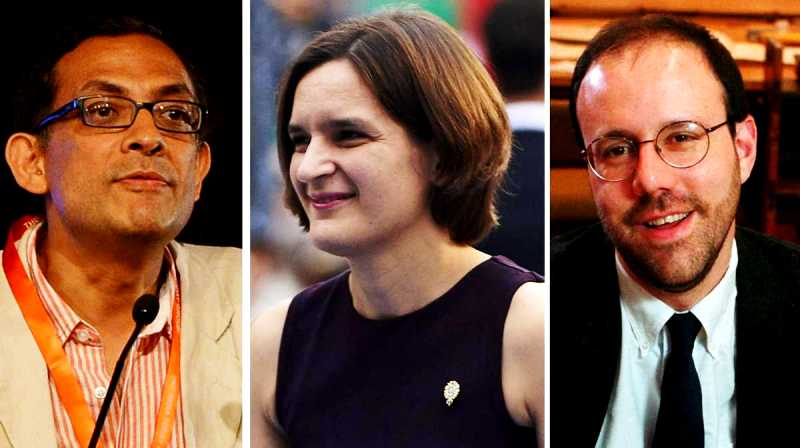
\includegraphics[height = 7cm]{ImpactEvaluation/figure/BanerjeeDufloKremer.jpg}\\
{\footnotesize 出所: \url{https://wikibio.in/abhijit-banerjee/}}
\end{frame}

\begin{frame}{祝: ノーベル経済学賞受賞3人(2019年)}
\begin{description}
\vspace{1.0ex}\setlength{\itemsep}{1.0ex}\setlength{\baselineskip}{12pt}
\item[Abhijit Banerjee]	インド人。理論経済学者。MIT教授。
\item[Esther Duflo]	フランス人。開発経済学者。MIT教授。
\item[Michael Kremer]	アメリカ人。理論経済学者。ハーバード大教授。
\end{description}
\vspace{2ex}
受賞理由: \\
「貧困緩和に実験的手法を導入した功績。貧困(という大きな)問題を小さな扱いやすい問題に分解し、実験を使って対策を示した。」
\end{frame}
\begin{frame}{祝: ノーベル経済学賞受賞3人(2019年)}
長所
\begin{enumerate}
\vspace{1.0ex}\setlength{\itemsep}{1.0ex}\setlength{\baselineskip}{12pt}
\pause
\item	歪みなく効果を計測できる(\textcolor{red}{internal validity})
\pause
\item	(結果に疑問を挟む余地は少ないので無駄な議論を節約できる)
\begin{dinglist}{45}\footnotesize
\vspace{1.0ex}\setlength{\itemsep}{1.0ex}\setlength{\baselineskip}{12pt}
\pause
\item	被験者をランダムに治療群the treatedと統御群the cotrolに割り振り、前者にのみ介入
\item	Randomisation of treatment: 治療群と統御群は相似、異なるのは介入の有無だけ
\item	結果指標の違いは介入が原因と解釈可能
\end{dinglist}
\end{enumerate}
\vspace{2ex}
\pause
貢献
\begin{enumerate}
\vspace{1.0ex}\setlength{\itemsep}{1.0ex}\setlength{\baselineskip}{12pt}
\item	政策の根拠を推測から科学的証拠に変えた: evidence based policy making
\pause
\item	研究者も証拠の質を議論するようになった
\pause
\item	実験可能な事象・研究が提示すべき証拠の質の基準を上げた$\rightarrow$転じて観察データを使う研究の対象を明確化
\end{enumerate}
\end{frame}
\begin{frame}{祝: ノーベル経済学賞受賞3人(2019年)}
例\\
%\vspace*{-1cm}
%\makebox[\linewidth]{
\includegraphics[page=1,width=\paperwidth]{paste0(path, "ImpactEvaluation/figure/fig2_ek_19_improved_educational_outcomes.pdf")}}\\
%\vspace{-13cm}
\hfil\makebox[\linewidth]{
\includegraphics[width=.75\paperwidth]{c:/seiro/docs/external/seishin/lec_slides/2024/ImpactEvaluation/figure/fig2_ek_19_improved_educational_outcomes.jpg}}\\
%\vspace{-13cm}

教科書無料配布よりも(ケニア西部)、無料学校給食よりも(ケニア西部)、習熟の遅い生徒に補習させる方が試験点数を上げることが分かった(インド、ムンバイ近郊)
\end{frame}
\begin{frame}[t]{祝: ノーベル経済学賞受賞3人(2019年)}
短所
\begin{enumerate}
\vspace{1.0ex}\setlength{\itemsep}{1.0ex}\setlength{\baselineskip}{12pt}
\item	メカニズム・理由(なぜ効果があったか)と無関係に実施可能。このため、理論を意識しなくても実験が可能。メカニズムが不明なので、その他地域への適用可能性(\textcolor{red}{external validity})が不明。
	\begin{itemize}
	\vspace{1.0ex}\setlength{\itemsep}{1.0ex}\setlength{\baselineskip}{12pt}
\pause
	\item	地域: インドで効果1ならガボンではどのくらいの効果?
\pause
	\item	実施主体: NGOは能力もモラルも高く、政策担当者と比較にならない
\pause
	\item	(該当する理論が存在しないときに先入観無しにできることが良いときもある)
	\end{itemize}
\pause
\item	大きな政策を扱えない。大規模実験(e.g., ジャムナ橋建設)は統御群をなくす。
\pause
\item	標本サイズが小さい($\leftarrow$予算がかかるから)ので推計値の精度が低い。参加率が低いと分析に使える標本がさらに減る。マイクロファイナンス実験。
\pause
\item	実験バイアス: Hawthorne effect (treated), John Henry effect (control; raced against machine)
\end{enumerate}
\end{frame}
\begin{frame}[t]{祝: ノーベル経済学賞受賞3人(2019年)}
短所
\begin{enumerate}
\setcounter{enumi}{4}
\vspace{1.0ex}\setlength{\itemsep}{1.0ex}\setlength{\baselineskip}{12pt}
\item	検討手段が実験可能なものに集中: 薬、職業訓練、教材、補助教員、肥料、携帯
	\begin{itemize}
	\vspace{1.0ex}\setlength{\itemsep}{1.0ex}\setlength{\baselineskip}{12pt}
	\pause
	\item	ランダム化しやすい: 親の学歴や年齢、家族構成は無理
	\pause
	\item	小さい(分割可能で被験者に割当可能): 橋や為替レートは無理
	\pause
	\item	倫理的に許要できる: 母乳育児、違法行為(贈賄: インド)推奨は駄目、政治デモ参加推奨(して参加人数計測)は文脈による\citep{Bursztyn2021}?
		\begin{dinglist}{43}
		\vspace{1.0ex}\setlength{\itemsep}{1.0ex}\setlength{\baselineskip}{12pt}
	\pause
		\item	かと思われたが、やはり、\href{https://www.pnas.org/doi/10.1073/pnas.2012021117}{批判されている}\citep[][``Should scholars be allowed to start a riot to see how violence spreads?'']{McDermottHatemi2020}。350香港ドル=45ドルくらい。
	\pause
		\item	\href{https://www.aeaweb.org/doi/10.1257/aeri.20200261.appx}{筆者たちの主張(オンライン付論)}: 
			\begin{itemize}
			\vspace{1.0ex}\setlength{\itemsep}{1.0ex}\setlength{\baselineskip}{12pt}
	\pause
			\item	4大学(Munich, Stanford, UC Berkeley, HKUST)のIRB承認を得ている
	\pause
			\item	リスクは小さい(10/15回で逮捕者ゼロ、2003年からのべ135万人が参加なのでデモ参加は日常から乖離せず、実験当時の2017-2018に言論の自由は保障されていた、軍による鎮圧可能性は小さい)\pause$\leftarrow$先読み感ゼロ、想像力が...当局が写真撮るかもよ?
			\end{itemize}
		\end{dinglist}
	\end{itemize}
\end{enumerate}
\end{frame}
\begin{frame}{祝: ノーベル経済学賞受賞3人(2019年)}
\begin{columns}[T]
\column{.2\paperwidth}
\vspace{2ex}鍵を捜す男
\column{.45\paperwidth}
\pause
\hfil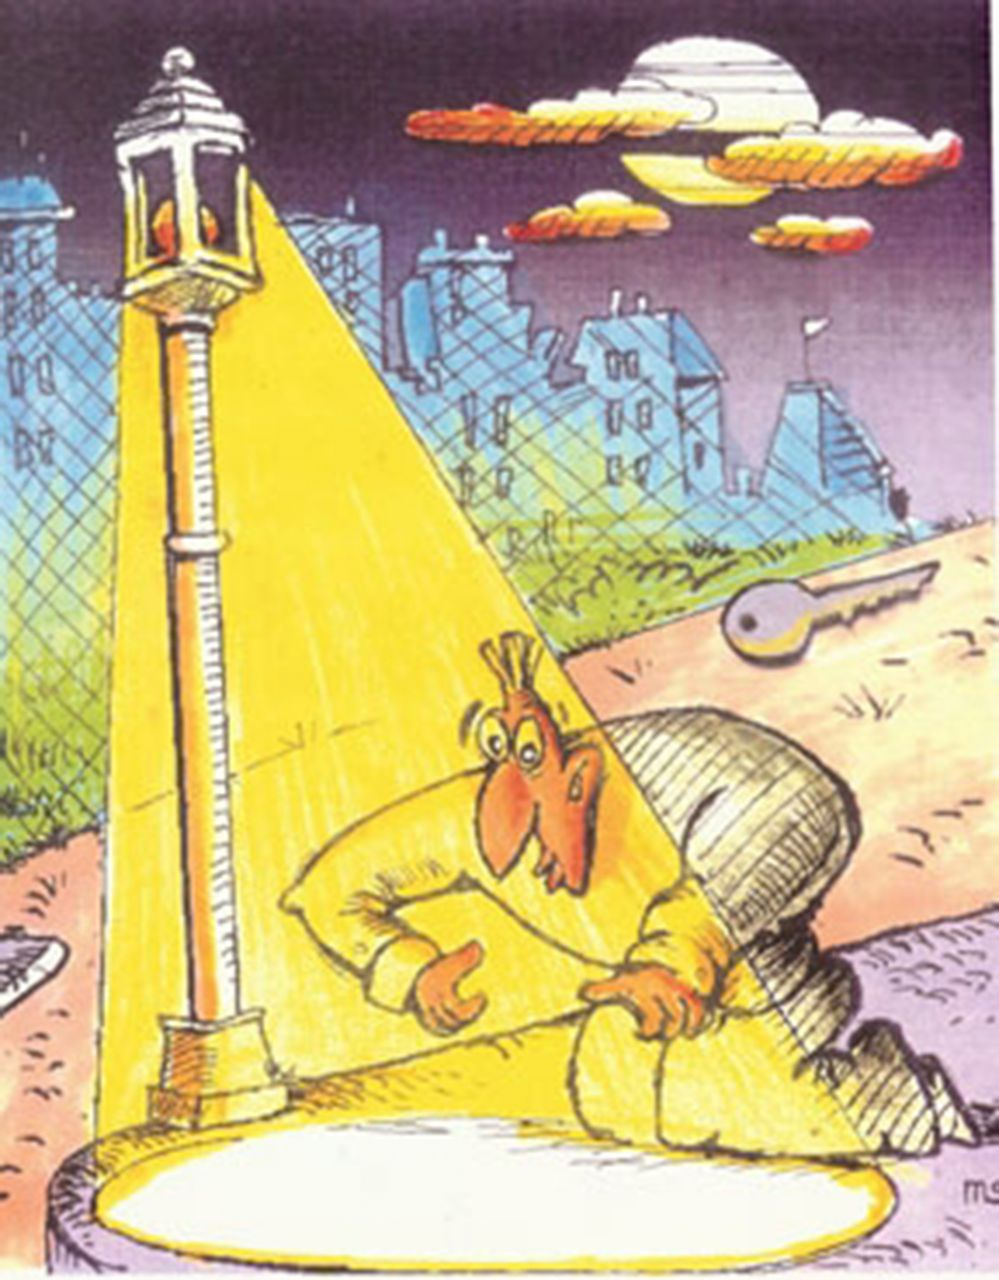
\includegraphics[height = 7cm]{ImpactEvaluation/figure/FindKey.jpg}
\column{.3\paperwidth}
{\footnotesize 出所: \url{https://diabetes.diabetesjournals.org/content/64/4/1105}}
\end{columns}
\end{frame}

\begin{frame}{}
倫理上、母乳育児や母乳育児に金銭的誘因を与える「推奨」を実験できないが、母乳育児の非金銭的「推奨」(内容伝達)を実験しても倫理的に問題ない\\~\\
\pause
ただし、推奨内容が比較対象の女性に伝わらないか統御は難しい\\~\\
\pause
実験がうまくいき、効果があると分かっても、政策に採用されるかは別問題\\~\\
\pause
政治家および投票基盤が政策実施=得策と思わねばならないから
\pause
\begin{dinglist}{43}
\vspace{1.0ex}\setlength{\itemsep}{1.0ex}\setlength{\baselineskip}{12pt}
\item	個別補習の費用対効果が最も大きい: %学習塾経営者は驚かないだろうが、教科書・参考書配布派、栄養補給派を説得するために証拠提示が必要だったのだろう。
学校教育の不十分さを示す結果。実験は学校教育の質の低さへの対症療法を示したが、根治療法を示していない。根治療法は教員・公務員組合等の反対で政治的に困難だろう。
\end{dinglist}
\vspace{3ex}
\pause
実験は思いついた政策に効果があるか気軽に試せるが、必要となる作業監理と予算は多いために、本当に検討する価値のある政策を選ばないと資源の無駄
\pause
\begin{dinglist}{43}
\vspace{1.0ex}\setlength{\itemsep}{1.0ex}\setlength{\baselineskip}{12pt}
\item	投与と反応を見る疫学研究ではなく、人々の意志決定と行動選択を含む経済学研究なので計測に費用がかかる
\end{dinglist}
\end{frame}

\begin{frame}{HA! HA! HA! HA!}
\begin{columns}[T]
\column{.6\paperwidth}
\hfil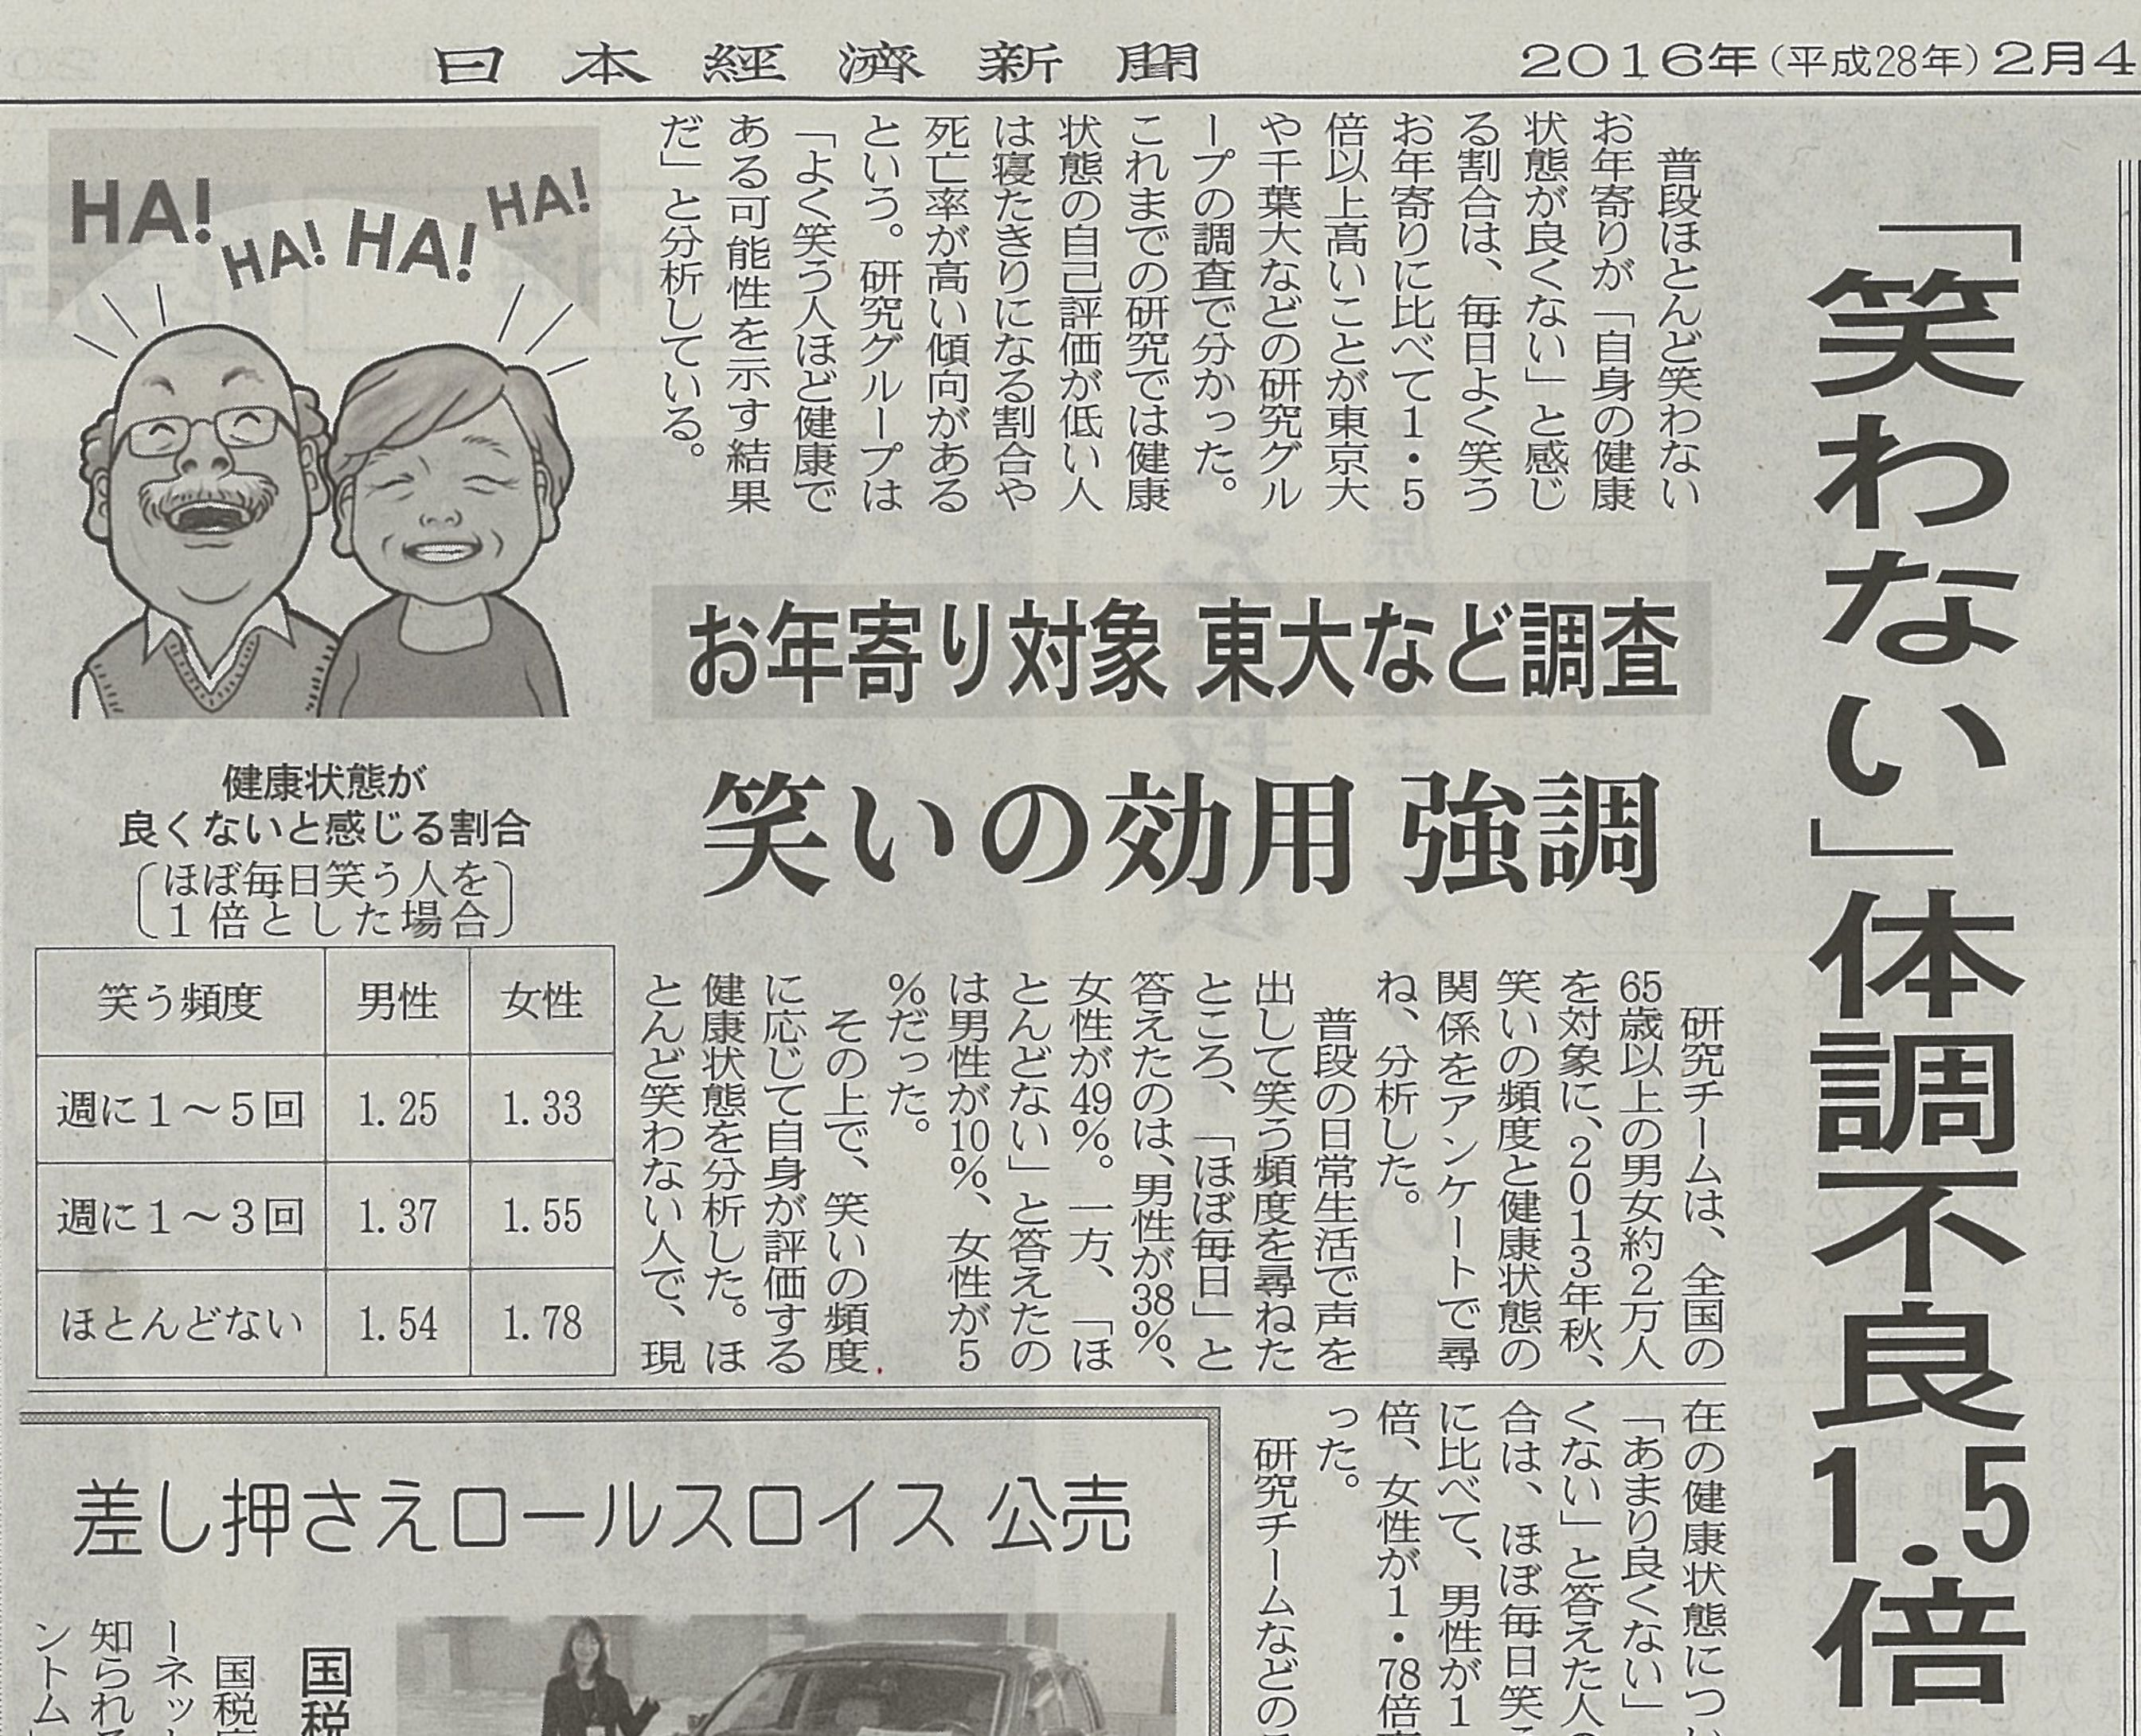
\includegraphics[height = 7cm]{ImpactEvaluation/figure/bad_graphs/hahaha0.eps}
\column{.35\paperwidth}
\begin{itemize}
\vspace{1.0ex}\setlength{\itemsep}{1.0ex}\setlength{\baselineskip}{12pt}
\item	高齢者: 笑う頻度が減ると健康不調を報告する比率が増える
\end{itemize}
\mpage{.3\paperwidth}{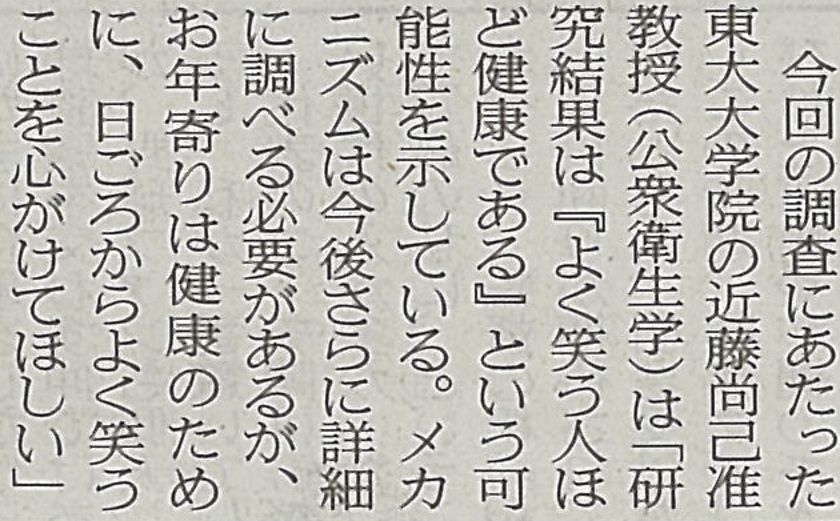
\includegraphics[width = .3\paperwidth]{ImpactEvaluation/figure/bad_graphs/hahaha1.eps}}
\end{columns}
\end{frame}


\begin{frame}{HA! HA! HA! HA!}
この記事には問題があります。何でしょうか。
\vspace{2ex}
\pause
問題を理解するためには、インパクト評価のキー・タームを知る必要があります
\end{frame}

\begin{frame}{HA! HA! HA! HA!}
\begin{description}[<+->]
\vspace{1.0ex}\setlength{\itemsep}{1.0ex}\setlength{\baselineskip}{12pt}
\item[因果causality]	$A\Rightarrow B$ (``A causes B.'')
\item[相関correlation]	$\corr[A, B]\neq 0$ (``A is correlated with B.'')
\end{description}

\pause
%A correlation between $A$ and $B$ can include multitude of cases.
$A$と$B$が相関: さまざまな因果関係があり得る

\vspace{4ex}
\hfil\begin{tikzpicture}
\path 
	(0, 1) node [shape = circle, draw, fill = blue!20] (A1) {$A$}
	(2, 1) node [shape = circle, draw, fill = red!20] (B1) {$B$};
\pause\draw [->, >= stealth'] (A1) -- (B1);
\pause\path 
	($(A1) + (3.5, 0)$) node [shape = circle, draw, fill = blue!20] (A2) {$A$}
	($(B1) + (3.5, 0)$) node [shape = circle, draw, fill = red!20] (B2) {$B$};
\pause\draw [->, >= stealth'] (B2) -- (A2);
\pause\path 
	($(A1) + (1.75, -1)$) node [shape = circle, draw, fill = blue!20] (A4) {$A$}
	($(B1) + (1.75, -1)$) node [shape = circle, draw, fill = red!20] (B4) {$B$};
\pause\draw [->, >= stealth'] ($(B4) + (-.4, .2)$) -- ($(A4) + (.4, .2)$); 
\draw [->, >= stealth'] ($(A4) + (.4, -.2)$) -- ($(B4) + (-.4, -.2)$);
\pause\path 
	($(A2) + (3.5, 0)$) node [shape = circle, draw, fill = blue!20] (A3) {$A$}
	($(B2) + (3.5, 0)$) node [shape = circle, draw, fill = red!20] (B3) {$B$}
	($(A3) + (1, -1)$) node [shape = circle, draw, fill = green!20] (C3) {$C$};
\pause\draw [->, >= stealth'] (C3) -- (A3); \draw [->, >= stealth'] (C3) -- (B3);
\node[below] at ($(C3) + (0, -.5)$) {見せかけの相関};
\end{tikzpicture}
\end{frame}

\begin{frame}{HA! HA! HA! HA!}
%Does laughter cause (self-reported) healthiness?
笑いは健康(自己申告)を引き起こすか?
\begin{itemize}[<+->]
\vspace{1.0ex}\setlength{\itemsep}{1.0ex}\setlength{\baselineskip}{12pt}
\item	可能性はある%Maybe. 
\item	もしくは、健康が笑いを引き起こす%Or healthiness can cause laugher.
\item	もしくは、その両方%Or both.
\end{itemize}

\pause
\vspace{2ex}
%Can the study design reveal causality?
この研究のデザインは因果関係を明らかにできるか?
\begin{itemize}
\vspace{1.0ex}\setlength{\itemsep}{1.0ex}\setlength{\baselineskip}{12pt}
\pause \item	できない。%No. 
\pause (なぜかはすぐに分かります)%You will see later why not.)
\end{itemize}

\vspace{2ex}
\pause %Then, can we say anything causal?
では、何でもいいので何らかの因果関係を示すことはできるか。
\begin{itemize}
\vspace{1.0ex}\setlength{\itemsep}{1.0ex}\setlength{\baselineskip}{12pt}
\pause \item	できない %No.
\end{itemize}
\end{frame}

\begin{frame}{HA! HA! HA! HA!}
\hfil
\includegraphics[clip, height = 8cm]{ImpactEvaluation/figure/bad_graphs/hahaha.eps}
\end{frame}


\begin{frame}{}
因果関係と相関関係は同じではない
\begin{itemize}
\vspace{1.0ex}\setlength{\itemsep}{1.0ex}\setlength{\baselineskip}{12pt}
\pause
\item	因果関係$\Rightarrow$相関関係
\pause
\item	相関関係$\Rightarrow$因果関係、ではない場合がある
\end{itemize}
\pause

\[
\begin{aligned}
\mbox{試験点数}&=20+20*D+e\\
D&=
\left\{
\begin{array}{c}
0\\
1
\end{array}
\right. \quad \mbox{if 塾に週1時間以上}
\left\{
\begin{array}{l}
\mbox{通わない}\\
\mbox{通う}
\end{array}
\right.
\end{aligned}
\]
$D$はダミー変数dummy variableと呼ばれる0と1の2つの値をとる離散変数。2つの値しかとらないので2項変数binary variableとも呼ばれる。ここでは塾に週1時間以上通うと1、そうではない場合は0という値をとる変数。塾に通う人と通わない人にグループ分けできる。$e$は誤差を表す確率変数で誤差項error termという。\\

\pause
\vspace{1ex}
ダミー変数は質的情報を表現できる: 
\begin{description}
\vspace{1.0ex}\setlength{\itemsep}{1.0ex}\setlength{\baselineskip}{12pt}
\pause
\item[背景に連続変数がある]	程度によるグループ分け。明るいと明るくない、早いと早くない、貧しいと貧しくない。
\pause
\item[背景に連続変数がない]	分類によるグループ分け。右利きと左利き、テレビとそれ以外の家電、男とそれ以外のジェンダー、日本人と外国人。
\end{description}
\end{frame}

\begin{frame}{}
\[
\mbox{試験点数}=20+20*D+e
\]
\pause
これが因果関係の場合: 塾に通う$\Rightarrow$点数が40点になる、という解釈になる。\\~\\
\pause
\vspace{1ex}
\hfil\begin{tikzpicture}[>=latex', shorten >=1pt, node distance=3cm, on grid, initial/.style={}]
  \node[state, minimum size = 1.75cm]				(juku)				[]
    {\footnotesize 塾通い};
  \node[state, minimum size = 1.75cm]				(tensuu)			[right = 8cm of juku]
    {\footnotesize 点数};
\tikzset{mystyle/.style={->, double=blue}} 
\tikzset{every node/.style = {}} 
\path (juku) edge[mystyle] node{} (tensuu);
\end{tikzpicture}
\end{frame}

\begin{frame}{}
でも、方程式は相関関係を表す場合もある。
\begin{itemize}
\vspace{1.0ex}\setlength{\itemsep}{1.0ex}\setlength{\baselineskip}{12pt}
\item	仮に、塾に試験点数を上げる効果は全く無いときに、勉強好きで試験点数がもともと20点程度良い人が勉強の機会を増やすために塾に行っている場合にも、この方程式は成り立つ。この場合、勉強好き$\Rightarrow$点数、勉強好き$\Rightarrow$塾通いという因果関係はあっても、塾通い$\Rightarrow$試験点数という因果関係はない。
\pause
「勉強好き」という欠落変数が試験点数と塾通いに同時に影響を与えていて、試験点数と塾通いの間に因果的な関係はない。
\end{itemize}

\vspace{1ex}
\pause

\hfil\begin{tikzpicture}[>=latex', shorten >=1pt, node distance=3cm, on grid, initial/.style={}]
  \node[state, minimum size = 1.75cm]				(juku)				[]
    {\footnotesize 塾通い};
  \node[state, minimum size = 1.75cm]				(tensuu)			[right = 8cm of juku]
    {\footnotesize 点数};
\pause
  \node[state, , minimum size = 1.75cm, dashed]	(benkyosuki)	[right = 4cm of juku, yshift = -1.5cm]
    {\footnotesize 勉強好き};
\tikzset{every node/.style = {}} 
%\path (juku) edge[mystyle] node{} (tensuu);
\tikzset{mystyle/.style = {->, double=orange}}
\path 
  (benkyosuki) edge[mystyle] node{} (juku)
  (benkyosuki) edge[mystyle] node{} (tensuu);
\end{tikzpicture}

\end{frame}

\begin{frame}{}
方程式は逆の因果関係を表す場合もある。
\begin{itemize}
\vspace{1.0ex}\setlength{\itemsep}{1.0ex}\setlength{\baselineskip}{12pt}
\item	仮に、試験点数が20点ほど良い人だけ選んで塾に行くことを強制しても、この方程式は成り立つ。
\pause
この場合、点数$\Rightarrow$塾通いという逆の因果関係が成り立っている。
\end{itemize}
\pause
\vspace{1ex}
\hfil\begin{tikzpicture}[>=latex', shorten >=1pt, node distance=3cm, on grid, initial/.style={}]
  \node[state, minimum size = 1.75cm]				(juku)				[]
    {\footnotesize 塾通い};
  \node[state, minimum size = 1.75cm]				(tensuu)			[right = 8cm of juku]
    {\footnotesize 点数};
\tikzset{mystyle/.style={->, double=blue}} 
\tikzset{every node/.style = {}} 
\path (tensuu) edge[mystyle] node{} (juku);
\end{tikzpicture}

\pause
\vspace{3ex}
方程式は必ずしも右辺$\Rightarrow$左辺の因果関係ばかりではなく、逆方向の因果関係や欠落変数を通じた相関関係も含む。

\end{frame}

\begin{frame}{}
因果関係を示すためには特定の条件が必要。その条件がない\textcolor{red}{\textbf{通常の回帰式の場合、相関関係まで}}しか読み取ることができない。\\~\\
\pause
\textcolor{red}{\textbf{予測だけなら相関関係で十分。}}塾に通う人は(なぜか分からないけど)試験点数が高い傾向がある、という関係だけで予測はできる。これは便利。\\~\\
\pause
でも、\textcolor{red}{\textbf{相関関係からは理由やメカニズム(因果関係の組み合わせ)は分からない。}}よって、何かの事情でメカニズムが変わった場合、相関関係の強さも変わって、それまで通りの予測はできなくなる。\\~\\
\pause
相関関係に頼った予測はメカニズムを検討しないため、理論なき計測measurement without a theoryと揶揄されることもある
\end{frame}

\begin{frame}{}
因果関係を示す方法: \textbf{ランダム化統御試験randomised controlled trial (RCT)}

\begin{itemize}
\vspace{1.0ex}\setlength{\itemsep}{1.0ex}\setlength{\baselineskip}{12pt}
\pause
\item	被験者・被験対象をランダムに「治療群(the treated)」「統御群(the control)」に割り振る
	\begin{dinglist}{43}
	\vspace{1.0ex}\setlength{\itemsep}{1.0ex}\setlength{\baselineskip}{12pt}
\pause
	\item	ランダムに割り振ったので、両群の試験点数(とその他変数)の分布(の特徴である平均値)はほぼ同じのはず%平均的な差はゼロのはず
\pause
	\item	標本が大きいほど誤差が減って平均値差はゼロに近づく
	\end{dinglist}
\pause
\item	治療群にのみ塾に通わせる
	\begin{dinglist}{43}
	\vspace{1.0ex}\setlength{\itemsep}{1.0ex}\setlength{\baselineskip}{12pt}
\pause
	\item	治療のspilloverを防ぐ: 統御群被験者が塾に通わないように、治療群被験者が塾に通うように、かつ、治療群被験者が統御群被験者に塾で学んだことを教えないように、被験者の行動を統御しなければいけない
\pause
	\item	でも、被験者はやりたいことをやるので、そうした不完全な制御の政策の効果を測定していると解釈
%	\item	RCTをやるのが大変な理由がこれ
	\end{dinglist}
\pause
\item	後日、試験をして採点する
\pause
\item	治療群の方が成績が高くなったら、塾に通う$\Rightarrow$試験点数が高い、という因果関係を示すことができる
% 	\begin{dinglist}{43}
% 	\vspace{1.0ex}\setlength{\itemsep}{1.0ex}\setlength{\baselineskip}{12pt}
% \pause
% 	\item	回帰式で表現したければ、両群の試験点数と塾通いの情報を集めて推計すれば良い。
% 	\end{dinglist}
\end{itemize}
\end{frame}

\begin{frame}{}
\setlength{\baselineskip}{20pt}
%Project evaluation used to casually state something like,\\
%インパクト評価や
プロジェクト評価の報告書にはさらっとこんな結論が散見される\\
%``with the project, health status improved.''
「プロジェクトによって健康状態が改善された」\\~\\
\pause
%What is the CF (with whom they are comparing)?
問うべきこと: Counterfactual(比較\underline{すべき}対象)は何か?\\~\\

\pause
問い直すべきこと: 比較\underline{している}対象は何か?\\

\pause
Before-after: 以前の自分
%Previous self.
\\

\pause
With-without: アクセスのない誰か
%Someone who does not have access.
\\~\\

\pause
%Is this a legit comparison?
インパクトを知る上で適切な比較か?\\~\\

\pause
%Almost always, no. (This is not to say that there are not cases these comparisons correctly give underlying impacts.)
殆どの場合、不適切
\end{frame}

\begin{frame}{}
%We can say a policy changed $y_{i}$ when we can compute its causal impact on $y_{i}$ as\\~\\
下記のようにインパクトを計測できれば、政策が結果指標$y_{i}$を変えたといえる\\~\\

%\hspace{2em}($y_{i}$ when $i$ is affected by the policy)\\
%\hspace{4em}$-(y_{i}$ when $i$ is not affected by the policy).\\~\\
\hspace{2em}($i$が政策に影響されたときの$y_{i}$)\\
\hspace{4em}$-(i$が政策に影響されなかったときの$y_{i}$).\\~\\
\pause
%If we use a mathematical notation, we can rewrite this as:
数学表記すると
\[
\begin{aligned}
(y_{i}|D_{i}=1) &- (y_{i}|D_{i}=0), \quad \mbox{or,}\\
y_{i1}&-y_{i0}.%, \quad y_{i0}=y_{i}|D=0, \ y_{i1}=y_{i}|D=1.
\end{aligned}
\]
\pause
\begin{description}
\vspace{0.0ex}\setlength{\itemsep}{1.0ex}\setlength{\baselineskip}{12pt}
\item[$D_{i}=0,1$]	%$D_{i}=1$ when $i$ belongs to the treated group (group affected by the policy), $D_{i}=0$ when $i$ belongs to the control group (group not affected by the policy). $D_{i}$ is called an \textit{indicator function} of ($i$ belongs to a group affected by) the policy or a \textit{dummy variable} of the policy.
$i$が治療群(政策に影響されるグループ)に属するとき$D_{i}=1$、$i$が統御群(政策に影響されないグループ)に属するとき$D_{i}=0$%$D_{i}$は$i$が政策に影響されるグループに属することのインディケータ関数\textit{indicator function} 、もしくは、政策に影響されるグループに属することのダミー変数\textit{dummy variable}。
\item[``$|$''] Reads ``given'' or ``when''. 「次が所与のとき」「次が成り立つとき」と読む
\item[$y_{i}|D_{i}=1$] $i$が治療群に属しているときの$y_{i}$、$y_{i1}$とも書く
\item[$y_{i}|D_{i}=0$] $i$が統御群に属しているときの$y_{i}$、$y_{i0}$とも書く
\end{description}
\end{frame}

\begin{frame}{}
%Treatment effect of policy for individual $i$:
個人$i$の治療効果treatment effect:
\[
(y_{i}|D_{i}=1)-(y_{i}|D_{i}=0)=
y_{1i}-y_{0i}.
\]
%The fundamental problem in program evaluation.
プログラム評価での根源的問題\\~\\
\pause
%We cannot observe $y_{i}$ in the treated and in the control for the same individual $i$ simultaneously.
治療群に属するときの$y_{i}$と統御群に属するときの$y_{i}$を同時に観察できない\\~\\
\pause
\hfil$\Leftrightarrow$\\
%We cannot observe a \textcolor{red}{\textit{counterfactual}} (CF) outcome for each individual $i$'s factual outcome.
各個人$i$の結果指標$y_{i}$の\textcolor{red}{\textit{counterfactual (CF)}}を観測することはできない\\~\\
\pause
%In other words, we cannot compute the causal impacts of a policy for each individual $i$ without further assumptions.
\hfil$\Leftrightarrow$\\
言い換えれば、仮定なしには政策の効果を計算することはできない
\pause
\begin{description}
\vspace{3.0ex}\setlength{\itemsep}{1.0ex}\setlength{\baselineskip}{12pt}
\item[$y_{i}|D_{i}=1$のCF] %An outcome $y_{i}$ if $i$ belongs to the control (``$y_{0i}$''), when in reality $i$ belongs to the treated ($D_{i}=1$). Write as $y_{0i}|D_{i}=1$. 
現実には治療群($D_{i}=1$)に属する$i$が統御群に属したときの結果指標$y_{i}$ (``$y_{0i}$'')。$y_{0i}|D_{i}=1$と表記。
\item[$y_{i}|D_{i}=0$のCF] %An outcome $y_{i}$ if $i$ belongs to the treated (``$y_{1i}$''), when in reality $i$ belongs to the control ($D_{i}=0$). Write as $y_{1i}|D_{i}=0$. 
現実には統御群($D_{i}=0$)に属する$i$が治療群に属したときの結果指標$y_{i}$ (``$y_{1i}$'')。$y_{1i}|D_{i}=0$と表記。
\end{description}
\vspace{1.0ex}
\end{frame}

\begin{frame}{}
%But under a certain set of assumptions, we can estimate the average causal impacts of a policy, the \textcolor{red}{average treatment effect (ATE)}.
一定の仮定の下、政策の\textcolor{red}{平均治療効果average treatment effect (ATE)}を推計できる
\[
ATE=\E[y_{i}|D_{i}=1]-\E[y_{i}|D_{i}=0].
\]
\\~\\
\pause
%Consider a thought experiment.
以下の思考実験を考える\\~\\

%Suppose there are a large number $n$ of individuals and we randomly assign the treatment status $D_{i}$ to everyone $i=1,\cdots, n$. Assume the randomisation was done well (i.e., based on ``a fair coin toss'').
多数$n$の個人に対し、ランダムに治療状態$D_{i}$をを割り当てる。ランダム化がうまくできたとする(公平なコインを使うなど).\\~\\

%The distribution of $y_{i}$ of each group should look very similar, or in the limit where $n\rightarrow\infty$, they are identical. If the distributions are very similar, then their means are also very similar. Write the mean in the limit as $\mu_{0}$.
両グループの$y_{i}$の分布は似通うはず。分布が近似していれば平均値も近似する。極限を取って$n\rightarrow\infty$($n$が無限大の場合)、両グループの分布は同一、平均値も同じになる。\\~\\
\end{frame}

\begin{frame}[label=ATEConsistencyCondition, t]{}
%Conditions that gave the ATE estimate consistency are
ATEを(一致推計量consistent estimator [標本が無限大になると真の値になる推計量]として)得る条件
\begin{enumerate}
\vspace{1.0ex}\setlength{\itemsep}{1.0ex}\setlength{\baselineskip}{12pt}
%\item	Distributions of $y_{i}$ of the control and the treated are very similar in the absence of a policy. \label{atecon1}
%\item	($n$ is sufficiently large.)\label{atecon2}
%\item	Impact is homogenous across $i$.\label{atecon3}
\item	政策前に、統御群と治療群の($y_{i}$)分布が近似していること。\label{atecon1}
\item	($n$が十分に大きいこと。)\label{atecon2}
\item	インパクトはすべての$i$で同じ。\label{atecon3}
\end{enumerate}

\pause
\vspace{1.0ex}
%\ref{atecon2} is the law of large numbers. In practice $n$ cannot be infinity, but a large enough sample size will mimic the sample average to $\mu_{0}$, the true mean.
\ref{atecon2}は大数の法則。現実に$n$は無限大よりも小さいが、十分に大きければ標本平均が母集団平均に十分近くなる。\\~\\

\pause
%\ref{atecon3} is used for simplification. If the impact is different across subgroups, we can use finer grouping.
\ref{atecon3}は単純化のために利用。グループごとにインパクトが違うなら、グループをもっと細かく分ければいい。\\~\\

\pause
%\ref{atecon1} is of most importance at this stage. It is randomisation of treatment status among individuals that gave similarity of distributions. 
\ref{atecon1}が最も重要。ランダムに割り振ることによって、各グループの特徴の分布が近似。\\~\\

\pause
%Whenever we can expect random assignment of treatment status, we can get a consistent estimate of ATE. E.g., clinical trials use explict randomisation between the treated and the placebo to get a consistent estimate of ATE.
グループの割り振りがランダムだと、ATEの一致推計量が得られる。
\begin{dinglist}{43}
\vspace{1.0ex}\setlength{\itemsep}{1.0ex}\setlength{\baselineskip}{12pt}
\item	ATEの一致推計量を得るために、治験は患者をプラセボ(統御群)と治療群にランダムに割り振る。
\end{dinglist}
\end{frame}

\begin{frame}[t, label=RCTProcedures]{}
実験をしてからの手順
\begin{enumerate}
\vspace{1.0ex}\setlength{\itemsep}{1.0ex}\setlength{\baselineskip}{12pt}
\item	ATEを推計 (estimation)
	\begin{itemize}
\pause
	\vspace{1.0ex}\setlength{\itemsep}{1.0ex}\setlength{\baselineskip}{12pt}
	\item	両群の平均値の差を計算
	\end{itemize}
\pause
\item	推計値を検定する統計学的推論 (inference)
	\begin{itemize}
	\vspace{1.0ex}\setlength{\itemsep}{1.0ex}\setlength{\baselineskip}{12pt}
\pause
	\item	帰無仮説「両群の平均値の差はゼロ」が正しい場合の分布を使って平均値の差が極端かを計算、計算する極端さの指標は$p$値
\pause
	\item	極端であれば帰無仮説に疑問を呈し、$p$の確率でATEはゼロではない、と推論
	\end{itemize}
\end{enumerate}
\pause
\begin{dinglist}{45}
\vspace{1.0ex}\setlength{\itemsep}{1.0ex}\setlength{\baselineskip}{12pt}
\item	$p$値($p$ value)は帰無仮説が成り立つ確率と考えていい
	\begin{dinglist}{43}\footnotesize
	\vspace{1.0ex}\setlength{\itemsep}{1.0ex}\setlength{\baselineskip}{10pt}
	\pause
	\item	正確には、帰無仮説が正しい下で推計値(この場合は平均値の差)が発生する確率
	\pause
	\item	この確率($p$値)が小さいとき、得られた推計値は帰無仮説から見て極端な事象\pause
	$\rightarrow$帰無仮説の正しさを疑うべき\pause
	$\rightarrow$帰無仮説が正しい確率は$p$値ほど小さい\\[2ex]
	\end{dinglist}
\pause
\item	$p$値が5\%をカットオフにして、5\%未満だったら「統計的に有意」、以上だったら「統計的に有意ではない」と表現されることが多いが、\textcolor{red}{推奨できない} $\leftarrow$ 4.99\%と5.01\%の差は無視可能なのに表現が違いすぎる
\end{dinglist}
\end{frame}

\begin{frame}[t, label=RCTProcedures]{}
実験をしてからの手順
\begin{enumerate}
\setcounter{enumi}{2}
\vspace{1.0ex}\setlength{\itemsep}{1.0ex}\setlength{\baselineskip}{12pt}
\item	推論の頑健性をチェック (robustness checks)
	\begin{itemize}
	\vspace{1.0ex}\setlength{\itemsep}{1.0ex}\setlength{\baselineskip}{12pt}
\pause
	\item	ランダム化の確認
		\begin{description}
		\vspace{1.0ex}\setlength{\itemsep}{1.0ex}\setlength{\baselineskip}{12pt}
\pause
		\item[Randomisation checks]	実験前の特徴が両群で似ていること=ランダム化が成功していることを検定、帰無仮説「実験前の(全)変数において、両群の平均値の差はゼロ」
		\end{description}
\pause
	\item	他要因排除の確認: 他要因による効果を検定。効果が見出されたら、メインの結論もその要因が引き起こしたかも。
		\begin{description}
		\vspace{1.0ex}\setlength{\itemsep}{1.0ex}\setlength{\baselineskip}{12pt}
\pause
		\item[Placebo tests]	介入変数を編集して、効果が無いことを検定(e.g., 一部controlに介入=1と割当てる、介入量doseを変える)
\pause
		\item[Falsification tests (negative controls)]	効果が発生し得ない標本や結果に介入=1と割当て、効果がないことを検定(e.g., 介入前の標本、ラマダン介入に影響され得ないラマダン下のキリスト教徒標本)
		\end{description}
		\begin{dinglist}{43}\footnotesize
		\vspace{1.0ex}\setlength{\itemsep}{1.0ex}\setlength{\baselineskip}{10pt}
\pause
		\item	両方ともほぼ同じ内容。敢えて言うならば、placebo testsはどんなデータでも実施可能、falsification testsは特定の文脈を使って実施。後者だけ実施可能な対象を狭める限定があるので、後者は前者に含まれる概念。
		\end{dinglist}
	\end{itemize}
\end{enumerate}
\end{frame}



\begin{frame}{}
ランダム化確認: permutation test (並べ替え検定), randomisation test (確率化検定)\\~\\
\pause
帰無仮説null hypothesis: グループaの分布=グループbの分布\\~\\
\pause
両グループのデータ全てを並べ、グループ名(a, b)をランダムに並べ替えてグループa平均値を計算。これを多数回繰り返すと、グループ``a''平均値の分布が描ける。\\~\\
\begin{columns}[T]
\column{.475\paperwidth}
\pause
帰無仮説が正しければ、本当のグループa平均値はグループ``a''平均値の分布の中央付近に位置するはず。\\~\\
\column{.475\paperwidth}
\pause
左右どちらかの端にあれば、グループaとグループbの分布は異なっていると判断できる。
\end{columns}
\pause
\begin{dinglist}{45}
\vspace{1.0ex}\setlength{\itemsep}{1.0ex}\setlength{\baselineskip}{12pt}
\item	$p$値($p$ value)は帰無仮説が成り立つ確率と考えていい
	\begin{dinglist}{43}\footnotesize
	\vspace{1.0ex}\setlength{\itemsep}{1.0ex}\setlength{\baselineskip}{10pt}
	\pause
	\item	正確には、帰無仮説が正しい下で推計値(この場合は平均値の差)が発生する確率
	\pause
	\item	この確率($p$値)が小さいとき、得られた推計値は帰無仮説から見て極端な事象\pause
	$\rightarrow$帰無仮説の正しさを疑うべき\pause
	$\rightarrow$帰無仮説が正しい確率は$p$値ほど小さい\\[2ex]
	\end{dinglist}
\end{dinglist}
\pause
平均値以外の(25\%)分位値などにも適用可。グループ``a''の(25\%)分位値を計算すれば同じ手順。グループ``a''(25\%)分位値分布の端に位置すると、両グループの(25\%)分位値が異なることを示唆する。
\end{frame}
{
\setbeamercolor{background canvas}{bg=gray!80!blue}
\setbeamercolor{normal text}{fg=black}
\begin{frame}{}
バングラデシュ最貧困層への貸付実験: 大規模貸付グループと小規模貸付グループの比較\\
\hfil\begin{minipage}[t]{12cm}
\hfil\textsc{\normalsize Permutation test results of arm assignment,}\\
\hfil\textsc{traditional vs. non-traditional arms\label{tab trad nontrad random assignment perm}}\\
\setlength{\tabcolsep}{.5pt}
\setlength{\baselineskip}{8pt}
\renewcommand{\arraystretch}{.50}
\hfil\begin{tikzpicture}
\node (tbl) {\input{c:/data/GUK/analysis/save/Original1600Memo3/RandomAssignmentTradNonTradPermutationTestResultso800.tex}};
\end{tikzpicture}\\
\begin{tabular}{>{\hfill\scriptsize}p{1cm}<{}>{\hfill\scriptsize}p{.25cm}<{}>{\scriptsize}p{10cm}<{\hfill}}
Source:& \multicolumn{2}{l}{\scriptsize Estimated with GUK administrative and survey data.}\\
Notes: & 1. & \textsf{R}'s package \textsf{coin} is used for baseline group mean covariates to conduct approximate permutation tests. \\
&2. & Number of repetition is set to 100000. Step-down method is used to adjust for multiple testing of a multi-factor grouping variable. 40 are lost to flood before arm assignment. 
\end{tabular}
\end{minipage}
\end{frame}
}


\begin{frame}{}
%Randomisation of treatment status will give us a consistent ATE estimate. 
治療対象選定をランダム化するとATEの一致推計量が得られる\\~\\

\pause
%But...\pause people have a right to choose. Choose not to get treated. What if everyone said ``No, I do not want to get treated''? 
でも...\pause 人々には同意するか決める権利がある。治療を断るかもしれない。全員が断ったらどうする?\\~\\
\pause
%Further...\pause people sometimes cheat. They will do stuffs that give them the treated status when they are assigned as the control. What if there is noncompliance? \\~\\
さらに...\pause 人々は時にずるをする。統御群に割り振られても何とかして治療群として参加するかもしれない。被験者が同意事項に違反するときどうする?\\~\\

\pause
%Except in North Korea, people have a right to choose. So we cannot force the assigned treatment status to the subjects. \\~\\
北朝鮮のような独裁国家以外では、人々には選ぶ権利がある。被験者にグループ割り振りを強制することはできない。\\~\\
\pause
%And experimenters are never perfect, so there may be noncompliers. 
実験者も完璧ではないので非同意者を必ず出してしまう\\~\\

\pause
%What we can measure is the mean group difference inclusive of noncompliance. Noncompliance makes estimated impact smaller. \\~\\
%This estimator is called \textcolor{red}{intention-to-treat (ITT)} effect, and is like a down-to-earth version of ATE. It is about \textit{effectiveness} (impacts in the field) rather than \textit{efficacy} (impacts in the lab).
われわれが計測できるのは非同意者を含むグループ平均値の差。非同意者がいるとインパクトが小さくなる。\\~\\
\pause
非同意者を含む効果推計値を\textcolor{red}{治療意図に基づく効果intention-to-treat (ITT) effect}という。実験室での効力\textit{efficacy}ではなくフィールドでの有効性\textit{effectiveness}。ATEを推計できる研究は少ない。
%Keiomobile2 pw	 hqhdaohuukknhisq

\end{frame}


\begin{frame}[label=ListOfEstimand, t]{}
さまざまな効果推計量(実証研究の大半がITTかLATE)
\begin{description}
\vspace{1.0ex}\setlength{\itemsep}{-1.0ex}\setlength{\baselineskip}{12pt}
\item[ATE]	Average treatment effects: 全個人の平均効果
\[
ATE = \E[y_{i}|D_{i}=1]-\E[y_{i}|D_{i}=01].
\]
\pause
\vspace{-1ex}
\item[ITT]	Intention-to-treat effects: 実施群非同意者(比率$1-\alpha\in[0, 1]$)と統御群非同意者(比率$1-\beta\in[0, 1]$)を含む全個人の平均効果, 実際の割当て$A_{i}=0, 1$
\[
\begin{aligned}
ITT
&= 
\alpha\E[y_{i}|D_{i}=1, A_{i}=1]+(1-\alpha)\E[y_{i}|D_{i}=1, A_{i}=0] \quad && \mpage{2.5cm}{\footnotesize \textcolor{green}{$\E[y_{i}|D_{i}=1]$}}\\
&\hspace{1em}-\beta\E[y_{i}|D_{i}=0, A_{i}=0]-(1-\beta)\E[y_{i}|D_{i}=0, A_{i}=1]. && \mpage{2.5cm}{\footnotesize \textcolor{green}{$-\E[y_{i}|D_{i}=0]$}}
\end{aligned}
\]
\pause
\vspace{-1ex}
\item[ATT]	Average treatment effects on the treated: 実施群における平均効果
\[
ATT = \E[y_{1i}|D_{i}=1]-\E[y_{0i}|D_{i}=1].
\]
\pause
\item[LATE]	Local average treatment effects: 割当てられて初めて介入を受ける同意者compliers ($\alpha-\beta$だけいる)の平均効果、均一効果$\E[\Delta y_{i}|D_{i}=1, A_{i}=1]=\E[\Delta y_{i}|D_{i}=0, A_{i}=0]=\mu$を仮定
\[
LATE = \frac{\alpha\E[\Delta y_{i}|D_{i}=1, A_{i}=1]-\beta\E[\Delta y_{i}|D_{i}=0, A_{i}=0]}{\alpha-\beta}
=
\frac{(\alpha-\beta)\mu}{\alpha-\beta}=\mu.
\]
\end{description}
\end{frame}



\begin{frame}{}
%\textcolor{red}{治療群の平均治療効果Average treatment effect on the treated}, (\textcolor{red}{ATT}, average treatment effect of only among the treated)
\textcolor{red}{治療群の平均治療効果Average treatment effect on the treated}, (\textcolor{red}{ATT}, 治療群における平均治療効果)
\[
ATT = \E[y_{1i}|D_{i}=1]-\E[y_{0i}|D_{i}=1].
\]
\pause
\begin{itemize}
\vspace{0.0ex}\setlength{\itemsep}{1.0ex}\setlength{\baselineskip}{12pt}
%\item	$y_{0i}|D_{i}=1$ is CF of the treated.
\item	$y_{0i}|D_{i}=1$治療群のCF
%\item	Difference between ATE and ATT:  The mean outcome difference among the treated or everyone.
\pause
\item	ATEとATTの違い:  全員 vs. 治療群
\pause	
\item	ITTとATTの違い: 非同意者を含む全員 vs. 治療群
%\item	$y_{1i}|D_{i}=1$ reads, outcome $y_{i}$ when $i$ is in the treated, when in fact $i$ is in the treated. I know the repetition is weird and redundant, and in math, redundancy is simply dropped, so it becomes simply as ``outcome $y_{i}$ when $i$ is in the treated.''
%\item	$y_{0i}|D_{i}=1$ reads, outcome $y_{i}$ when $i$ is in the control, when in fact $i$ is in the treated. So it is a hypothetical outcome $y_{i}$ outside the policy impacts, when in fact $i$ is affected by the policy. So it becomes ``outcome $y_{i}$ if $i$ was in the control, when in reality $i$ is in the treated.''
\end{itemize}

\vspace{1ex}
\pause
%Analgously, we can define ATC (average treatment effects on the control) as
統御群の平均治療効果average treatment effects on the control (ATC)も以下のように定義できる
\[
ATC = \E[y_{1i}|D_{i}=0]-\E[y_{0i}|D_{i}=0].
\]
\pause
%ATE is a weighted average of ATT and ATC.
ATEはATTとATCの加重平均値
\[
ATE = b ATT + (1-b) ATC, \quad b= \frac{n_{1}}{n_{0}+n_{1}}.
\]
\end{frame}

\begin{frame}[t, label=Targeting]{}
\renewcommand{\arraystretch}{1}
\hfil\begin{tabular}{
>{\hfil}p{.5cm}<{}
>{\hfil}m{.5cm}<{}
>{\hfil}m{3cm}<{}
>{\hfil}m{3cm}<{}
}
&&\multicolumn{2}{c}{裨益}\\
&& \cellcolor{blue!30}No & \cellcolor{blue!30}Yes\\
\multirow{2}{*}{\rotatebox{90}{\makebox[2.0cm]{ターゲット対象}}}&\rotatebox{90}{\cellcolor{blue!30}\makebox[1.25cm]{No}}& compliers & \only<3->{\cellcolor{red!20}}\temporal<3>{}{\textcolor{red}{leakage}}{leakage}\\
&\rotatebox{90}{\cellcolor{blue!30}\makebox[1.25cm]{Yes}}& \only<4->{\cellcolor{red!20}}\temporal<4>{}{\textcolor{red}{exclusion}}{exclusion} & compliers\\[2.0ex]
\end{tabular}\\

\begin{itemize}
\vspace{1.0ex}\setlength{\itemsep}{1.0ex}\setlength{\baselineskip}{12pt}
\item	ターゲティング(対象設定)が正しくても、実現するかは別問題
\item	LATE: compliers (Yes, Yes) - compliers (No, No)
\end{itemize}

\end{frame}


\begin{frame}{}
\begin{columns}[T]
\column{.6\paperwidth}
LATE\\
\hfil\textbf{\footnotesize A Numerical Example}\\
\renewcommand{\arraystretch}{1.2}
\hfil\begin{tabular}{|>{\footnotesize$}c<{$}>{\footnotesize$}l<{$}>{\footnotesize$}c<{$}|
>{\hfil\footnotesize$}p{3em}<{$}>{\hfil\footnotesize$}p{3em}<{$}|
>{\footnotesize$}c<{$}>{\footnotesize$}c<{$}|}
\hline
&&& \multicolumn{2}{c|}{\textsc{\footnotesize treatment}}&& \\
&&& D=0 & D=1 & \bar{D}_{z} & \bar{y}_{z}\\\hline
\multirow{1}{.2cm}{ \rotatebox{90}{\textsc{\footnotesize \hfil eligibility}}} 
& z=0 & n_{0} & 80 & 20 & 0.20 & \\
& & y_{0} & 1000 & 2000 & & 1200\\[1ex]
& z=1 & n_{1} & 50 & 200 & 0.80 & \\
& & y_{1} & 1000 & 2000 & & 1800\\\hline
& & \bar{y}_{D}& 1000 & 2000 &\multicolumn{2}{c|}{\footnotesize $ITT=600$}\\\hline
\end{tabular}
\column{.35\paperwidth}
\pause
$ATE=1000=2000-1000=(y|D=1)-(y|D=0)$. \\~\\
\pause
$ITT=\bar{y}_{1}-\bar{y}_{0}=1800-1200=600$. \\~\\
\pause
Difference in participation rates\\
$\Delta \bar{D}_{z}=\bar{D}_{1}-\bar{D}_{0}=.8-.2=.6$.
\end{columns}
\pause
\vspace{2ex}
ITT per participant=ATE (only holds when impacts are homogenous).
\pause
\[
\frac{\bar{y}_{1}-\bar{y}_{0}}{\bar{D}_{1}-\bar{D}_{0}}
=
\frac{ITT}{\Delta \bar{D}_{z}}
=\frac{600}{.6}=1000.
\]
This is not ATE but called LATE. 
\end{frame}

\begin{frame}{}
\hypertarget{FIG WALD}{\scriptsize \bf Figure \refstepcounter{figure}\thefigure: 
A graphical representation of ITT and LATE (Wald estimator)
}\\

\begin{columns}[T]
\column{.5\paperwidth}
\hfil\begin{minipage}[t]{.5\paperwidth}
\begin{center}
\label{fig wald}

\vspace{-4ex}
\setlength{\unitlength}{.75mm}
\begin{picture}(120, 110)
\linethickness{.1mm}
\put(60, 10){\line(0, 1){95}}
\put(10, 50){\line(1, 0){100}}
\put(110, 48){\scriptsize $z$}
\put(59, 107){\scriptsize $y$}
\put(60, 50){\circle*{2}} \put(62, 51){\scriptsize $O$}

\onslide<2->{
\put(8, 48){\scriptsize $D$}
\put(59, 7){\scriptsize $D$}
\put(60, 50){\line(-1, -1){30}}
}
\onslide<3->{
\put(95, 25){\circle*{2}} \put(96, 51){\scriptsize 1}  \put(97, 24){\scriptsize $\bar{D}_{1}$}
\multiput(94, 25)(-2, 0){30}{\line(-1, 0){1}}
\multiput(95, 25)(0, 2){35}{\line(0, 1){1}} \put(21.5, 51){\scriptsize 1}
\put(95, 95){\circle*{2}} \put(97, 95){\scriptsize $\bar{y}_{z=1}$}
\multiput(93.5, 95)(-2, 0){30}{\line(-1, 0){1}}
%\multiput(24, 95)(0, -2){41}{\line(0, -1){1}}
\multiput(60, 14)(2, 0){18}{\line(1, 0){1}} \multiput(95, 14)(0, 2){5}{\line(0, 1){1}} 
\put(58, 15){\scriptsize 1}
\multiput(35, 25)(0, 2){35}{\line(0, 1){1}}
\put(35, 95){\circle*{2}} 
}
\onslide<4->{
\put(60, 40){\circle*{2}} \put(62, 39){\scriptsize $\bar{D}_{0}$}
\multiput(61, 40)(-2, 0){6}{\line(-1, 0){1}}
\put(60, 60){\circle*{2}} \put(62, 60){\scriptsize $\bar{y}_{z=0}$}
\multiput(50, 40)(0, 2){10}{\line(0, 1){1}}
\put(50, 60){\circle*{2}}
\multiput(60, 60)(-2, 0){13}{\line(-1, 0){1}}
}
\onslide<5->{
\put(61, 48.5){\vector(0,-1){7}} \put(62, 45){\tiny leakage}
\pause
\put(61, 15){\vector(0,1){9}} \put(62, 19){\tiny exclusion}
\pause
\put(61, 30){\vector(0,1){8}} \put(61, 30){\vector(0,-1){4}}  
\put(62, 34){\tiny $z$-induced}
\put(62, 32){\tiny participants}
% \put(62, 34){\tiny differences in}
% \put(62, 32){\tiny treatment} 
% \put(62, 30){\tiny explained by $z$}
}
\onslide<6->{
\put(61, 80){\vector(0,1){14}} \put(61, 80){\vector(0,-1){18}} 
\put(62, 76){\tiny $ITT$}
% \put(62, 80){\tiny differences in}
% \put(62, 78){\tiny outcomes} 
% \put(62, 76){\tiny explained by $z$}
}
\onslide<7->{
\linethickness{.3mm}
\put(48, 59){\textcolor{orange}{\vector(-1, 0){12}}} 
\put(33.5, 61){\textcolor{orange}{\vector(0, 1){32}}} 
}
\end{picture}
\end{center}
\end{minipage}
\column{.45\paperwidth}
\begin{itemize}
\vspace{1.0ex}\setlength{\itemsep}{1.0ex}\setlength{\baselineskip}{12pt}
\onslide<3->{\item	$z=1$の参加率$\bar{D}_{1}$と結果平均値$\bar{y}_{1}$}
\onslide<4->{\item	$z=0$の参加率$\bar{D}_{0}$と結果平均値$\bar{y}_{0}$}
\onslide<5->{
\item	Defiers: 
	\begin{itemize}\scriptsize
	\vspace{1.0ex}\setlength{\itemsep}{1.0ex}\setlength{\baselineskip}{10pt}
	\item	$z=1$で参加しない人たち=``exclusion'', $1-\bar{D}_{1}$
	\item	$z=0$で参加する人たち=``leakage'', $\bar{D}_{0}$、資格無くても参加する人たち
	\item	$z=0\rightarrow 1$によって参加する人たち=``$z$-induced partcipants'' $\bar{D}_{1}-\bar{D}_{0}$
	\end{itemize}
}
\end{itemize}
\begin{description}
\vspace{1.0ex}\setlength{\itemsep}{1.0ex}\setlength{\baselineskip}{12pt}
\onslide<6->{
\item[ITT]	$\bar{y}_{1}-\bar{y}_{0}$
}
\onslide<7->{
\item[LATE]	$z=0\rightarrow 1$になることで参加する$\bar{D}_{1}-\bar{D}_{0}$1人当たりの効果推計$\frac{ITT}{\mbox{$z$-induced participants}}=\frac{\bar{y}_{1}-\bar{y}_{0}}{\bar{D}_{1}-\bar{D}_{0}}$
}
\end{description}
\end{columns}
\end{frame}



\begin{frame}[label=KoreanAdopteeExperiment, t]{}
実験には人が意図して実施する科学実験と偶然発生する自然実験natural experimentsがある\\~\\

\pause
科学実験は非倫理的なものは実施しない\\~\\

\pause
自然実験は意図せず発生するので非倫理的であっても実施されてしまう
\begin{dinglist}{43}
\vspace{1.0ex}\setlength{\itemsep}{1.0ex}\setlength{\baselineskip}{12pt}
\pause
\item	チャンス!
\end{dinglist}

\vspace{2ex}
\pause
非倫理的な自然実験の例:
\begin{dinglist}{45}
\vspace{1.0ex}\setlength{\itemsep}{1.0ex}\setlength{\baselineskip}{12pt}
\item	妊婦のアルコール摂取\citep{Nilsson2017}
\item	胎内での経済的・心的ショック\citep{PerssonRossinSlater2018}
\item	親の変更\citep{FagerengMogstadRonning2021}
\end{dinglist}
\end{frame}

\begin{frame}[t]{}
親の違いによる子の純資産額、所得、学歴、金融投資への影響\\~\\

\citet{FagerengMogstadRonning2021}: 韓国の生活苦の乳児が養子縁組でノルウェイに行く\\~\\

\pause
NGO: ノルウェイで養親候補を書類審査+面接、合格者の書類を韓国に送付、先着順で子どもと縁組\\~\\

\pause
養親は子どもに関する希望を出せず、到着順はランダム\\~\\
\pause
養親は年齢、学歴、所得、純資産額などで異なる
\begin{dinglist}{43}
\vspace{1.0ex}\setlength{\itemsep}{1.0ex}\setlength{\baselineskip}{12pt}
\pause
\item	子にとっては親がランダムに変更される
\pause
\item	親のこれら特徴+その他をランダムに変える実験
\end{dinglist}

\vspace{2ex}
\pause
ランダムであることの確認: 
\pause
養子全員がtreatedなのでpermutation testは使えない
\begin{itemize}
\vspace{1.0ex}\setlength{\itemsep}{1.0ex}\setlength{\baselineskip}{12pt}
\pause
\item	NGOの手続き説明書類
\pause
\item	養子の特徴(月齢と性別)が養親の特徴と無相関: 養子の特徴を養親の特徴に回帰、推計された係数が統計学的にゼロ(帰無仮説: 係数はゼロ、が棄却できず)
\end{itemize}
\end{frame}

\begin{frame}[t]{}
親の違いによる子の純資産額、所得、学歴、金融投資への影響\\~\\

\begin{columns}[T]
\column{.5\paperwidth}
\hfil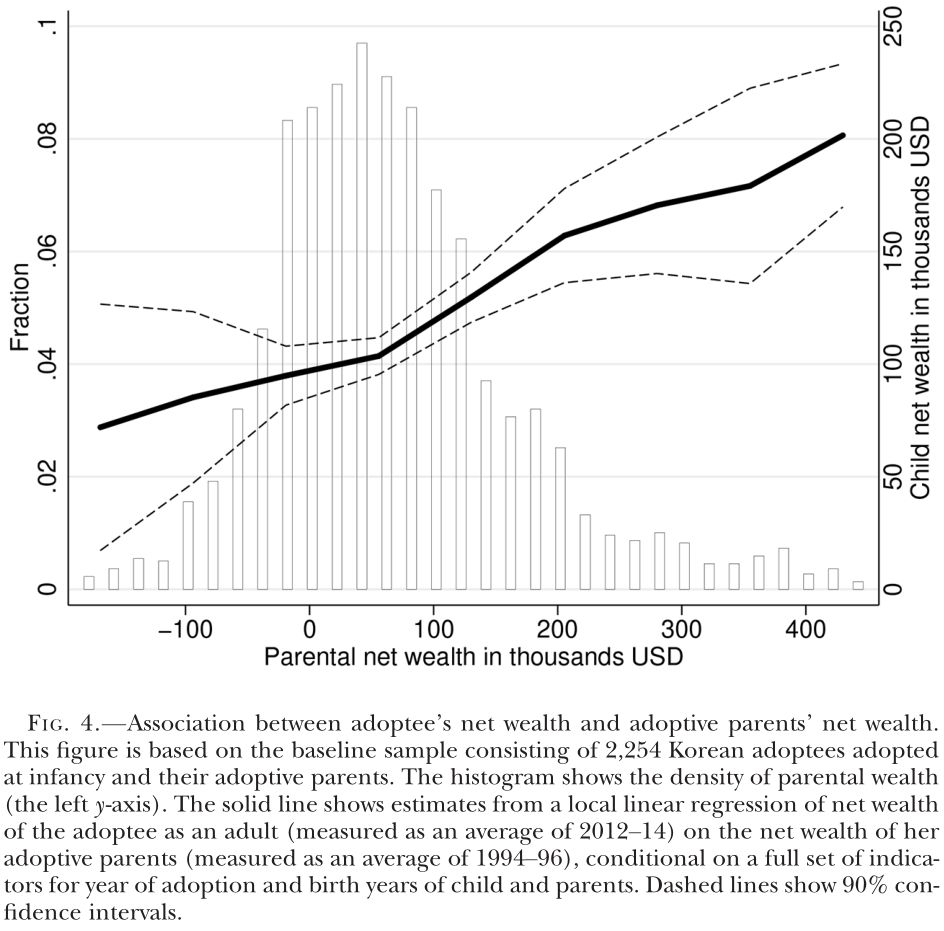
\includegraphics[clip, height = 7cm]{ImpactEvaluation/figure/FMR_Fig4.jpg}
\column{.45\paperwidth}
\begin{itemize}
\vspace{1.0ex}\setlength{\itemsep}{1.0ex}\setlength{\baselineskip}{12pt}
\pause
\item	右上がり: 養親の純資産額が増える$\Rightarrow$養子の純資産額が増える(右縦軸)
	\begin{dinglist}{43}
	\vspace{1.0ex}\setlength{\itemsep}{1.0ex}\setlength{\baselineskip}{12pt}
\pause
	\item	実線: 推計値
\pause
	\item	破線: 95\%信頼区間(95\% confidence interval)
	\end{dinglist}
\pause
\item	養親の純資産額の度数分布(左縦軸)
	\begin{dinglist}{43}
	\vspace{1.0ex}\setlength{\itemsep}{1.0ex}\setlength{\baselineskip}{12pt}
\pause
	\item	標本が多い(度数が多い)資産額では信頼区間が狭い=推計値の精度が高い
	\end{dinglist}
\end{itemize}

\end{columns}
\end{frame}

\begin{frame}[t]{}
親の違いによる子の純資産額、所得、学歴、金融投資への影響\\~\\

養子$i$の特徴$Y_{i}$と養親$j$の$k+1$個の特徴$W_{j}, x_{1j}, \dots, x_{kj}$がどのように関係しているかを見たい (養親純資産額は$W_{j}$, 養子の特徴も$m$個: $x_{1i}, \dots, x_{mi}$)
\begin{dinglist}{45}
\vspace{1.0ex}\setlength{\itemsep}{1.0ex}\setlength{\baselineskip}{12pt}
\pause
\item	特徴: 学歴、年齢、性別、所得、リスク資産投資比率など
\end{dinglist}

\vspace{1ex}
\pause
実験 $\rightarrow$ 養子にとって養親の特徴はランダムに与えられている
\begin{dinglist}{43}
\vspace{1.0ex}\setlength{\itemsep}{1.0ex}\setlength{\baselineskip}{12pt}
\pause
\item	実験の場合に限り、OLS(普通の回帰式)で歪みのない効果が推計できる
\end{dinglist}
\[
\begin{aligned}
Y_{i}
&=
\overbrace{\alpha_{1965}Z_{1965}+\cdots+\alpha_{1986}Z_{1986}}^{\mbox{\scriptsize adoption year effects}}+\textcolor{red}{\beta} W_{j} && \mbox{\footnotesize \textcolor{azure}{1965年の効果$+\cdots+$1986年の効果}}\\
&\hspace{1em}
+\underbrace{\eta_{1}x_{1j}+\cdots+\eta_{k}x_{kj}}_{\mbox{\scriptsize 養親の特徴の効果}}
+\underbrace{\lambda_{1}x_{1i}+\cdots+\lambda_{m}x_{mi}}_{\mbox{\scriptsize 養子の特徴を制御}} \hspace{0em}&& \mbox{\footnotesize \textcolor{azure}{\mpage{6cm}{就学年数の効果$+$養親のX歳効果$+$養子のX歳効果$+$縁組み日齢の効果$+$兄弟人数の効果$+$所得1単位増えることの効果$+$居住地域所得中央値の効果}}}\\[-3ex]
&\hspace{1em}
+\overbrace{\gamma\kappa_{j}+\delta\chi_{i}}^{\mbox{\scriptsize 養親と養子の固定効果}}+u_{i}.
\end{aligned}
\]
$\textcolor{red}{\beta}$: 養親から養子への純資産額の伝播係数
\end{frame}

\begin{frame}[t]{}
親の違いによる子の純資産額、所得、学歴、金融投資への影響\\
\begin{columns}[T]
\column{.65\paperwidth}
\begin{tikzpicture}[inner sep=0pt, remember picture]
\node at (0, 0) {
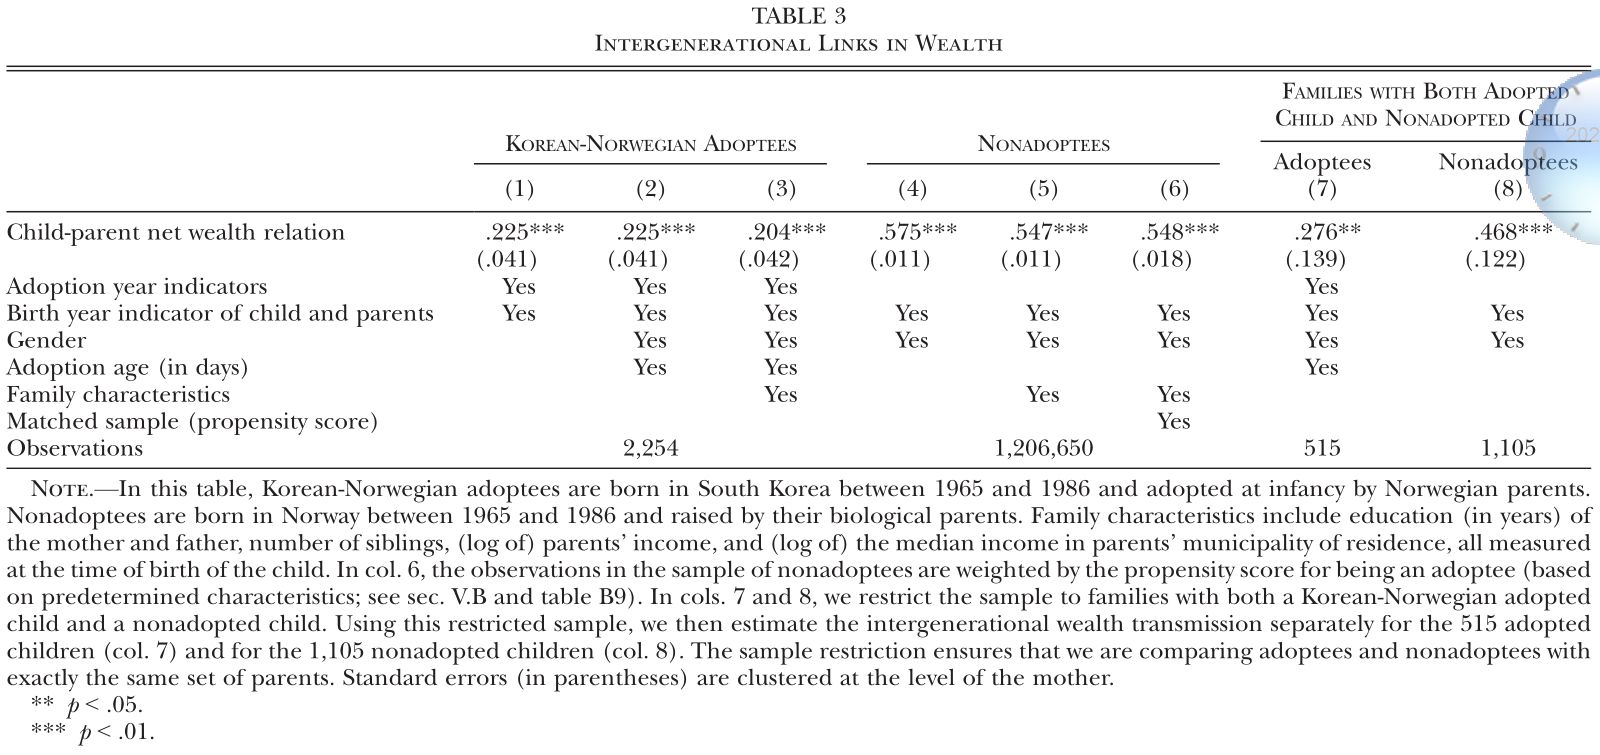
\includegraphics[clip, height = 5cm]{ImpactEvaluation/figure/FMR_Tab3.jpg}
};
\coordinate (h1) at (-2.2, 1.1);
\onslide<2->{
  \node (H1) [rectangle, anchor = south west, thick, rounded corners, minimum height = .6cm, 
    minimum width = 2.4cm, fill = azure, draw=azure, fill opacity=.1] at (h1){};
}
\onslide<3->{
  \node (H2) [rectangle, anchor = south west, thick, rounded corners, minimum height = .6cm, 
    minimum width = 2.4cm, fill = azure, draw=azure, fill opacity=.1, xshift = 2.6cm] at (h1){};
}
\onslide<5->{
  \node (H4) [rectangle, anchor = south west, thick, rounded corners, minimum height = .4cm, 
    minimum width = 1.0cm, fill = azure, draw=azure, fill opacity=.1, xshift = 5.2cm] at (h1){};
}
\onslide<6->{
  \node (H5) [rectangle, anchor = south west, thick, rounded corners, minimum height = .4cm, 
    minimum width = 1.0cm, fill = azure, draw=azure, fill opacity=.1, xshift = 6.3cm] at (h1){};
}
\onslide<7->{
  \node (H6) [rectangle, anchor = south west, thick, rounded corners, minimum height = .38cm, 
    minimum width = 7.2cm, fill = red, draw=red, fill opacity=.1, yshift = -.43cm] at (h1){};
}
\onslide<9->{
  \node (H8) [rectangle, anchor = south west, thick, rounded corners, minimum height = .2cm, 
    minimum width = 7.2cm, fill = green, draw=green, fill opacity=.1, yshift = -1.675cm] at (h1){};
}
\onslide<10->{
  \node (H9) [rectangle, anchor = south west, thick, rounded corners, minimum height = .4cm, 
    minimum width = 1.0cm, fill = darkgreen, draw=darkgreen, fill opacity=.1, xshift = -3.0cm, yshift = -3.6cm] at (h1){};
}
\end{tikzpicture}

\column{.3\paperwidth}\footnotesize
養親純資産額$\Rightarrow$養子純資産額\\~\\
\begin{tikzpicture}[inner sep=0pt, remember picture]
\onslide<2->{\node (hh1) at (1, -3) {\mpage{.3\paperwidth}{\footnotesize 
(1)-(3)韓国出自の養子
}};}
\onslide<3->{\node (hh2) at (1, -3.35) {\mpage{.3\paperwidth}{\footnotesize 
(4)-(6)実子
}};}
\onslide<4->{\node (hh3) at (1, -4.0) {\mpage{.3\paperwidth}{\footnotesize 
韓国出自の養子のいる家庭の
}};}
\onslide<5->{\node (hh4) at ($(hh3)+(-1.6, -.4)$) {\footnotesize 
(7)養子と
};}
\onslide<6->{\node (hh5) at ($(hh4)+(2.2, 0)$) {\footnotesize 
(8)実子のサンプル
};}
\onslide<7->{\node (hh6) at (1, -5.0) {\mpage{.3\paperwidth}{\footnotesize 
推計値と標準誤差
}};}
\onslide<8->{\node (hh7) at (1, -5.35) {\mpage{.3\paperwidth}{\footnotesize 
その他共変数
}};}
\onslide<9->{\node (hh8) at (1, -5.7) {\mpage{.3\paperwidth}{\footnotesize 
標本サイズ
}};}
\onslide<10->{\node (hh9) at (1, -6.5) {\mpage{.3\paperwidth}{\footnotesize 
$** p<.05$, $*** p<.01$は$p$ valueを示す
}};}
\end{tikzpicture}
\begin{tikzpicture}[remember picture, overlay]
\onslide<2->{
  \draw[azure, very thick, arrows={latex-}, ->] (hh1.west) to[out=120, in=70, looseness = 1] (H1.north);
}
\onslide<3->{
  \draw[azure, very thick, latex-, ->] (hh2.west) to[out=150, in=90, looseness = 1] (H2.north);
}
\onslide<5->{
  \draw[azure, very thick, latex-, ->] (hh4.north) to[out=70, in=80, looseness = 1] (H4.north);
}
\onslide<6->{
  \draw[azure, very thick, latex-, ->] (hh5.north) to[out=70, in=80, looseness = 1] (H5.north);
  }
\onslide<7->{
  \draw[red, very thick, latex-, ->] (hh6.west) to[out=180, in=0, looseness = 1] (H6.east);
}
\onslide<9->{
  \draw[green, very thick, latex-, ->] (hh8.west) to[out=180, in=-90, looseness = 1] (H8.south);
}
\onslide<10->{
  \draw[darkgreen, very thick, latex-, ->] (hh9.west) to[out=180, in=0, looseness = 1] (H9.east);
  }
\end{tikzpicture}
\end{columns}

\vspace{2ex}
\onslide<11->{
\begin{columns}[T]
\column{.4\paperwidth}
(1)-(3)の係数: .204 - .225
\column{.55\paperwidth}
養親の純資産額が5クローネ増えると養子の純資産額を(少なくとも)1クローネ増やす\\~\\
\end{columns}
}
\onslide<12->{
\begin{columns}[T]
\column{.4\paperwidth}
\pause
(4)-(6)の係数: .547 - .575
\column{.55\paperwidth}
養親の純資産額が5クローネ増えると実子の純資産額を(少なくとも)2.5クローネ増やす
\end{columns}
}
\end{frame}

\begin{frame}[t]{}
純資産額の効果は60\%程度が直接効果、40\%程度が間接効果(養子の所得、学歴、養子への生前贈与、経済系の学位)を経由\\~\\
\begin{dinglist}{43}
\vspace{1.0ex}\setlength{\itemsep}{1.0ex}\setlength{\baselineskip}{12pt}
\pause
\item	間接効果の80\%が生前贈与
\pause
\item	逆に言えば、養子の純資産額は68\%くらい(直接効果の60\%+40\%の2割)が生前贈与以外のもの
\end{dinglist}

\vspace{2ex}
\pause
養親の純資産額は養子の学歴は僅少効果、所得には統計学的にはゼロの効果
\begin{dinglist}{43}
\vspace{1.0ex}\setlength{\itemsep}{1.0ex}\setlength{\baselineskip}{12pt}
\pause
\item	ノルウェイが高学歴でより平等な社会だから差が出なかったのか?
\end{dinglist}

\vspace{2ex}
\pause
ただし、リスク資産投資比率は養親から養子に直接効果あり\\~\\

\pause
所得や学歴以外の家庭内の何かが子の純資産額を高める
\begin{dinglist}{43}
\vspace{1.0ex}\setlength{\itemsep}{1.0ex}\setlength{\baselineskip}{12pt}
\pause
\item	学校ではない...学校教育は平等化装置ではない(ノルウェイでは)
\pause
\item	何かが分からない...何をすれば貧しい家庭の子どもが同じリソースにアクセスできるのか
\end{dinglist}
\end{frame}

\begin{frame}{selection}
%When the treatment assignment ($D_{i}$) is not randomised, except for very rare lucky cases, the distributions of outcome measure in the absense of a policy are different between the treated and the control. \\~\\
グループの割り振り($D_{i}$)がランダム化していないと、ごく稀なケースを除き、政策がない場合の結果指標の分布はグループ間で異なる。\\~\\

\pause
%This is because we are dealing with humans who participate purposefully. \\~\\
被験者=目的意識を持って参加する人間なので、参加者と不参加者は特徴が異なる\\~\\

\pause
\begin{description}[<+->]
\vspace{1.0ex}\setlength{\itemsep}{1.0ex}\setlength{\baselineskip}{12pt}
%\item[self-selection]	 Selection by potential participants. People with a positive net participation benefit choose to participate.
\item[自己選抜self-selection]	 対象者自身による選抜。参加利益のある人は参加。
%\item[placement selection]	Selection by policymakers. If a policymaker is incentivised or instructed to choose a particular group, there is no guarantee that the distributions of outcome measures in the absence of a policy become similar between the treated (chosen) and the control (unchosen).
\item[実施対象選抜placement selection]	政策担当者による選抜。政策担当者が特定の集団を選ぶように指示もしくは誘因を得ているとき、政策がないときに対象者(治療群)と非対象者(統御群)の分布が近似する保証はない。
\end{description}
%As in the microfinance example, policy impacts (participation benefits) are expected to be correlated with the outcomes in the absence of a policy. Thus the distributions are different. In the absence of randomisation, if we take $D_{i}$ as we observe and compare between them, we end up comparing apples with oranges.
\end{frame}


\setcounter{angle}{0}
\newcounter{r}
\newcommand{\escalar}[1]{\setcounter{r}{#1 * #1 * #1}}
\newcounter{m}
\setcounter{m}{0}
\newcounter{mc}



\begin{frame}{self-selection}
%\def\beforeline{(0, 3) parabola bend (5,4) (8, 4.44)}
What we will learn:
\begin{enumerate}
\vspace{1.0ex}\setlength{\itemsep}{1.0ex}\setlength{\baselineskip}{12pt}
\item	Mechanism of self-selection
\item	Bias of the na\"ive estimator (simple comparison among treated and control)
\item	Difference-in-differences (DID) estimator and how before-after data of both treated and control can give a consistent estimate of ATT under a mild condition
\end{enumerate}
\end{frame}

\def\xlow{3.83}
\def\xadd{1.87}
\def\xpivot{3.2}
\def\xpivothalf{1.6}
\def\xpivothalftwo{5.6}
\def\xright2{4.5}
%\def\xpivothalf{\divide \xpivot by 2}
%\def\divider{2}
%\def\xpivothalf{\xpivot / \divider}
%\def\beforeline{(0, 3) to [out=20, in=-170] (8, \xright2) }
%\def\afterline{(0, 3)  to [out=45, in=-170] (8, 7.5)}
\def\beforeline{(0, 3) to [bend left = 5] (8, \xright2) }
\def\afterline{(0, 3)  to [bend left = 17] (8, 7.5)}
\setbeamercovered{invisible}


\begin{frame}{self-selection (benefits)}
%\def\beforeline{(0, 3) parabola bend (5,4) (8, 4.44)}
\begin{center}
	\begin{tikzpicture}[scale=1]
\onslide<1->{
		\draw[->] (0, 3) -- (9, 3) node[right] {ability};
		\draw[->] (0, 3) -- (0, 8) node[above] {outcome};
}
\onslide<2->{
		\draw[green, thick, -] \beforeline node[below right] {before};
}
\onslide<3->{
		\draw[azure, thick, -] \afterline node[above right] {after};
}
		%\foreach \x in {1, 2,..., 9}
		%\draw[shift={(\x, 3)}] (0pt, 2pt) -- (0pt, -2pt);
		%\foreach \y in {1, 2,..., 5}
		%\draw[shift={(0, 3+\y)}] (2pt, 0pt) -- (-2pt, 0pt); 
		%	pause for shaded area
\onslide<4->{
		\fill[blue, path fading=myfade]  (8, 7.5) to (8, \xright2)
		to [bend right=5] (0, 3) to [bend left=17] (8, 7.5);
		\node at (0, 3) [xshift = 5cm, yshift = 2.5cm]{\textbf{benefits}};
		\draw[green, thick, -] \beforeline node[below right] {before};
		\draw[azure, thick, -] \afterline node[above right] {after};
		\draw[->] (0, 3) -- (9, 3) node[right] {ability};
		\draw[->] (0, 3) -- (0, 8) node[above] {outcome};
}
      	\end{tikzpicture}
\end{center}
\end{frame}



\tikzstyle{shadingcosts} = [left color=gray!90, right color=gray!80, opacity = .3]
\tikzstyle{shadingcostsTwo} = [left color=gray!90, right color=gray!80, opacity = .12]
\begin{frame}{self-selection (costs)}
\begin{center}
	\begin{tikzpicture}[scale=1]
		%	participation costs
		\draw[->,  >=stealth'] (0, 3) -- (9, 3) node[right] {ability};
		\draw[->,  >=stealth'] (0, 3) -- (0, 8) node[above] {outcome};
		\draw[- ] (0, \xlow) -- (8.5, \xlow);
		\draw[- ] (0, \xlow + \xadd) -- (8.5, \xlow + \xadd);
		\pause
		\shade[shadingcosts] (0, \xlow) rectangle +(8.5, \xadd);
		\draw[](0, \xlow) node[xshift = 5cm, yshift = 1cm]{\textbf{participation costs}};
      	\end{tikzpicture}
\end{center}
\end{frame}

\begin{frame}{self-selection (benefits and costs)}
\begin{center}
	\begin{tikzpicture}[scale=1]
		\fill[blue, path fading=myfade]  (8, 7.5) to (8, \xright2)
		to [bend right=5] (0, 3) to [bend left=17] (8, 7.5);
		\node at (0, 3) [xshift = 5cm, yshift = 2.5cm]{\textbf{benefits}};
		\draw[green, thick, -] \beforeline node[below right] {before};
		\draw[azure, thick, -] \afterline node[above right] {after};
		\draw[->] (0, 3) -- (9, 3) node[right] {ability};
		\draw[->] (0, 3) -- (0, 8) node[above] {outcome};
		\shade[shadingcosts] (0, \xlow) rectangle +(8.5, \xadd); 
		\draw[-] (0, \xlow) -- (8.5, \xlow);
		\draw[-] (0, \xlow + \xadd) -- (8.5, \xlow + \xadd);
		\draw[](0, \xlow) node[xshift = 5cm, yshift = 1cm]{\textbf{participation costs}};
      	\end{tikzpicture}
\end{center}
\end{frame}


\def\beforelinesecondhalf{(\xpivot, \xlow) to [out=10, in=-170] (8, 4.5)}
\begin{frame}{self-selection (participation decisions)}
\begin{center}
	\begin{tikzpicture}[scale=1]
		\fill[blue, path fading=myfade]  (8, 7.5) to (8, \xright2)
		to [bend right=5] (0, 3) to [bend left=17] (8, 7.5);
		\node at (0, 3) [xshift = 5cm, yshift = 2.5cm]{\textbf{benefits}};
		\draw[azure, thick, -] \afterline node[above right] {after};
		\only<1>{\shade[shadingcosts] (0, \xlow) rectangle +(8, \xadd); }
		\draw[](0, \xlow) node[xshift = 5cm, yshift = 1cm]{\textbf{participation costs}};
		\draw[green, thick, -] \beforeline node[below right] {before};
		\draw[->] (0, 3) -- (9, 3) node[right] {ability};
		\draw[->] (0, 3) -- (0, 8) node[above] {outcome};
		\pause
		\shade[shadingcosts] (0, \xlow) rectangle +(\xpivot, \xadd); 
		\fill[shadingcostsTwo]  (\xpivot, \xlow+\xadd) to (8, \xlow+\xadd)
		  to (8, \xright2) to [bend right=2] (\xpivot, \xlow);
		\fill[shadingcostsTwo]  (\xpivot, \xlow+\xadd) to[bend left=.75] (8, \xlow+\xadd + \xright2 - \xlow)
		  to (8, \xlow+\xadd) to (\xpivot, \xlow+\xadd);
		\draw[green, thick, dashed] (\xpivot, \xlow+\xadd) to [out=10, in=-170] 
			(8, \xlow+\xadd + \xright2 - \xlow);
		\draw[green, thick, -] \beforeline node[below right] {before};
		\pause
		\draw[dashed] (\xpivot, 3) -- (\xpivot, 8) node[left] {do not participate} node[right] {participate};
      	\end{tikzpicture}
\end{center}
\end{frame}


\def\beforelinefirsthalf{(0, 3) to [out=20, in=-172] (\xpivot, \xlow)}
\def\afterlinesecondhalf{(\xpivot, \xlow+\xadd) to [out=32, in=-170] (8, 7.5)}
\def\afterlinefirsthalf{(0, 3) to [out=45, in=-145] (\xpivot, \xlow + \xadd)}
\begin{frame}{self-selection (results)}
\begin{center}
	\begin{tikzpicture}[scale=1]
		\draw[->] (0, 3) -- (9, 3) node[right] {ability};
		\draw[->] (0, 3) -- (0, 8) node[above] {outcome};
		\draw[name path=befmid, draw = none] (\xpivothalf, 3.2) -- (\xpivothalf, 8);
		\draw[name path=befone, thick, -] \beforelinefirsthalf;
		\draw[name path=contCF, draw = none] \afterlinefirsthalf;
		\draw[name path=treatCF, draw = none] \beforelinesecondhalf;
		\draw[name path=aftmid, draw = none] (\xpivothalftwo, 3.2) -- (\xpivothalftwo, 8);
		\draw[name path=aftone, thick, -] \afterlinesecondhalf;
		\draw[name path=befmean, draw = none] (4, 3.2) -- (4, 8);
		\pause
		\path[name intersections= {of=befone and befmid, by = int1}]; 
			\coordinate[label = below: {}] (b1) at (int1);
			\node[fill = black!10!white, inner sep = 2pt] at (b1){};
			\draw ($(b1) + (0, -1.75ex)$) node{\scriptsize$\E[y_{0}|D=0]$};
		\path[name intersections= {of=aftone and aftmid, by = int2}]; 
			\coordinate[label = above:{}] (a1) at (int2);
			\node[fill = black!10!white, inner sep = 2pt] at (a1){};
			\draw ($(a1) + (-2ex, 2ex)$) node{\scriptsize$\E[y_{1}|D=1]$};
		\pause
		\draw[dashed] (a1) -- ($(a1) - (4.2, 0)$);
		\draw[purple, thick, densely dashed, double, > = latex, <->] 
			($(a1) - (4.2, 0)$) -- ($(b1) - (.2, 0)$) 
			node[left = 1pt, pos = .45]{\scriptsize na\"{i}ve}
			node[left = 1pt, pos = .55]{\scriptsize comparison};
		\pause
		\draw[blue, dashed, thick] \afterlinefirsthalf;
		\draw[blue, dashed, thick] \beforelinesecondhalf;
		\path[name intersections= {of=contCF and befmid, by = int3}]; 
			\coordinate[label = below: {}] (a2) at (int3);
			\node[fill = black!10!white, inner sep = 2pt] at (a2){};
			\draw ($(a2) + (5ex, -.0ex)$) node{\scriptsize$\E[y_{1}|D=0]$};
		\path[name intersections= {of=treatCF and aftmid, by = int4}]; 
			\coordinate[label = above:{}] (b2) at (int4);
			\node[fill = black!10!white, inner sep = 2pt] at (b2){};
			\draw ($(b2) + (1ex, -2ex)$) node{\scriptsize$\E[y_{0}|D=1]$};
		\pause
		\draw[red, ultra thick, > = latex, <->] (b1) -- (a2) 
			node[right = 2pt, pos = .5]{\scriptsize ATC};
		\draw[red, ultra thick, > = latex, <->] (b2) -- (a1) 
			node[right = 2pt, pos = .5]{\scriptsize ATT};
		\pause
		\path[name intersections= {of=treatCF and befmean, by = int5}]; 
			\coordinate[label = below: {}] (b3) at (int5);
			\node[fill = black!10!white, inner sep = 2pt] at (b3){};
			\draw ($(b3) + (0ex, -2.0ex)$) node{\scriptsize$\E[y_{0}]$};
		\path[name intersections= {of=aftone and befmean, by = int6}]; 
			\coordinate[label = above:{}] (a3) at (int6);
			\node[fill = black!10!white, inner sep = 2pt] at (a3){};
			\draw ($(a3) + (-1ex, 1.5ex)$) node{\scriptsize$\E[y_{1}]$};
		\draw[red, ultra thick, > = latex, <->] (a3) -- (b3) 
			node[right = 2pt, pos = .5]{\scriptsize ATE};
      	\end{tikzpicture}
\end{center}
\end{frame}

\def\rectwidth{1.5}
\begin{frame}{self-selection (what we observe)}
\begin{center}
\begin{tikzpicture}
	%	coordinates for 
	\coordinate (befCorigin) at (1, 3);
	\coordinate (aftCorigin) at (5, 3);
	\coordinate (aftTorigin) at (5, 5.7);
	%	axises
	\draw[->] (0, 2.5) -- (0, 8) node[above] {outcome};
	\draw[-, dashed, gray!40] (0, 3) -- (7, 3) node[right] {0};
	\draw[->] (0, 2.5) -- (7, 2.5) node[right] {sequence};
	%	sequence of events and background shading
	\pause
	\node (x1) at ($(befCorigin) + (.75, -1)$) {\footnotesize before};
	\node (x2) at ($(befCorigin) + (2.75, -1)$) {\phantom{\footnotesize decision}};
	\node (x3) at ($(aftCorigin) + (.75, -1)$) {\phantom{\footnotesize after}};
	\filldraw[color = gray!50, opacity = .3] ($(aftCorigin) + (-4, -.5)$) 
		rectangle +(\rectwidth, 5.75);
	\pause
	\draw[> = latex, thick, ->] (x1) -- (x2);
	\pause
	\node (x2) at ($(befCorigin) + (2.75, -1)$) {\footnotesize decision};
	\filldraw[color = orange!50, opacity = .3] ($(befCorigin) + (1.5, -.5)$) 
		rectangle ($(aftCorigin) + (0, 5.25)$);
	\pause
	\draw[> = latex, thick, ->] (x2) -- (x3);
	\pause
	\node (x3) at ($(aftCorigin) + (.75, -1)$) {\footnotesize after};
	\filldraw[color = gray!50, opacity = .3] ($(aftCorigin) + (0, -.5)$) 
		rectangle +(\rectwidth, 5.75);
	%	control tukey plot
	\pause
	\draw[-] ($(aftCorigin) + (.75, 0)$) -- 
		($(aftCorigin) + (.75, .83)$) node[above] {do not participate};
		\filldraw[shading = ball, ball color = green] 
			($(aftCorigin) + (0, .2075)$) rectangle +(\rectwidth, .405);
		\draw[-] (aftCorigin) -- ($(aftCorigin) + (\rectwidth, 0)$);
		\draw[-] ($(aftCorigin) + (0, .83)$) -- 
			($(aftCorigin) + (\rectwidth, .83)$);
	%	treated tukey plot
	\pause
	\draw[-] ($(aftTorigin) + (.75, 0)$) -- 
		($(aftTorigin) + (.75, 1.8)$) node[above] {participate};
		\filldraw[ball color = darkred, shading = ball] 
			($(aftTorigin) + (0, .45)$) rectangle +(\rectwidth, .9);
		\draw[-] (aftTorigin) -- ($(aftTorigin) + (\rectwidth, 0)$);
		\draw[-] ($(aftTorigin) + (0, 1.8)$) -- 
			($(aftTorigin) + (\rectwidth, 1.8)$);
	%	before tukey plot
	\pause
	\draw[-] ($(befCorigin) + (.75, 0)$) -- 
		($(befCorigin) + (.75, 1.5)$) node[above] {before};
		\filldraw[shading = ball] ($(befCorigin) + (0, .375)$) 
			rectangle +(\rectwidth, 0.75);
		\draw[-] (befCorigin) -- ($(befCorigin) + (\rectwidth, 0)$);
		\draw[-] ($(befCorigin) + (0, 1.5)$) -- 
			($(befCorigin) + (\rectwidth, 1.5)$);
	%	arrows
	\pause
	\draw[->, ultra thick, ] ($(befCorigin) + (\rectwidth + .05, .75)$)
		to [out = -20, in = -170] ($(aftCorigin) + (-.2, .415)$);
	\pause
	\draw[->, ultra thick] ($(befCorigin) + (\rectwidth + .05, .75)$)
		to [out = 20, in = 170]  ($(aftTorigin) + (-.1, .9)$);
	%	dummy arguments
        		\draw [white, ultra thick, >= latex, <->]
	($(aftCorigin) + (\rectwidth + .5, .84+.28)$) --
	($(aftTorigin) + (\rectwidth + .5, .9)$) 
	node[left = 1pt, pos = .5] {\phantom{\scriptsize ATT}};
	%	naive
	\draw [white, ultra thick, >= latex, <->]
	($(aftCorigin) + (\rectwidth + .75, .415)$) --
	($(aftTorigin) + (\rectwidth + .75, .9)$) 
	node[right = 1pt, pos = .45] {\phantom{\scriptsize 単純な}};
	node[right = 1pt, pos = .55] {\phantom{\scriptsize 比較}};

\end{tikzpicture}
\end{center}
\end{frame}

\begin{frame}{evaluation: na\"ive comparison}
\begin{center}
\begin{tikzpicture}
	%	coordinates for 
	\coordinate (befCorigin) at (1, 3);
	\coordinate (aftCorigin) at (5, 3);
	\coordinate (aftTorigin) at (5, 5.7);
	%	axises
	\draw[->] (0, 2.5) -- (0, 8) node[above] {outcome};
	\draw[-, dashed, gray!40] (0, 3) -- (7, 3) node[right] {0};
	\draw[->] (0, 2.5) -- (7, 2.5) node[right] {sequence};
	%	sequence of events and background shading
	\node (x1) at ($(befCorigin) + (.75, -1)$) {\footnotesize before};
	\node (x2) at ($(befCorigin) + (2.75, -1)$) {\footnotesize decision};
	\node (x3) at ($(aftCorigin) + (.75, -1)$) {\footnotesize after};
	\filldraw[color = gray!50, opacity = .3] ($(aftCorigin) + (-4, -.5)$) 
		rectangle +(\rectwidth, 5.75);
	\draw[> = latex, thick, ->] (x1) -- (x2);
	\filldraw[color = orange!50, opacity = .3] ($(befCorigin) + (1.5, -.5)$) 
		rectangle ($(aftCorigin) + (0, 5.25)$);
	\draw[> = latex, thick, ->] (x2) -- (x3);
	\filldraw[color = gray!50, opacity = .3] ($(aftCorigin) + (0, -.5)$) 
		rectangle +(\rectwidth, 5.75);
	%	control tukey plot
	\draw[-] ($(aftCorigin) + (.75, 0)$) -- 
		($(aftCorigin) + (.75, .83)$) node[above] {do not participate};
		\filldraw[shading = ball, ball color = green] 
			($(aftCorigin) + (0, .2075)$) rectangle +(\rectwidth, .405);
		\draw[-] (aftCorigin) -- ($(aftCorigin) + (\rectwidth, 0)$);
		\draw[-] ($(aftCorigin) + (0, .83)$) -- 
			($(aftCorigin) + (\rectwidth, .83)$);
	%	treated tukey plot
	\draw[-] ($(aftTorigin) + (.75, 0)$) -- 
		($(aftTorigin) + (.75, 1.8)$) node[above] {participate};
		\filldraw[ball color = darkred, shading = ball] 
			($(aftTorigin) + (0, .45)$) rectangle +(\rectwidth, .9);
		\draw[-] (aftTorigin) -- ($(aftTorigin) + (\rectwidth, 0)$);
		\draw[-] ($(aftTorigin) + (0, 1.8)$) -- 
			($(aftTorigin) + (\rectwidth, 1.8)$);
	%	before tukey plot
	\draw[-] ($(befCorigin) + (.75, 0)$) -- 
		($(befCorigin) + (.75, 1.5)$) node[above] {before};
		\filldraw[shading = ball] ($(befCorigin) + (0, .375)$) 
			rectangle +(\rectwidth, 0.75);
		\draw[-] (befCorigin) -- ($(befCorigin) + (\rectwidth, 0)$);
		\draw[-] ($(befCorigin) + (0, 1.5)$) -- 
			($(befCorigin) + (\rectwidth, 1.5)$);
	%	dummy arguments
        		\draw [white, ultra thick, >= latex, <->]
	($(aftCorigin) + (\rectwidth + .5, .84+.28)$) --
	($(aftTorigin) + (\rectwidth + .5, .9)$) 
	node[left = 1pt, pos = .5] {\phantom{\scriptsize ATT}};
	%	naive
	\draw [white, ultra thick, >= latex, <->]
	($(aftCorigin) + (\rectwidth + .75, .415)$) --
	($(aftTorigin) + (\rectwidth + .75, .9)$) 
	node[right = 1pt, pos = .45] {\phantom{\scriptsize 単純な}};
	node[right = 1pt, pos = .55] {\phantom{\scriptsize 比較}};

	%	parenthesis
	\pause
        	\draw [gray, ultra thick, >= latex, <->]
			($(aftTorigin) + (\rectwidth + .05, .9)$) .. controls 
			 ($(aftTorigin) + (\rectwidth + .5, -.8)$) .. 
			($(aftCorigin) + (\rectwidth + .05, .415)$)
			node [right = .1pt, midway, yshift = 3.25pt] 
				{\scriptsize 比べては}
			node [right = .1pt, midway, yshift = -3.25pt] 
				{\scriptsize ダメ};
\end{tikzpicture}
\end{center}
\end{frame}

\begin{frame}{evaluation: proper comparison}
\begin{center}
\begin{tikzpicture}
	%	coordinates for 
	\coordinate (befCorigin) at (1, 3);
	\coordinate (aftCorigin) at (5, 3);
	\coordinate (aftTorigin) at (5, 5.7);
	%	axises
	\draw[->] (0, 2.5) -- (0, 8) node[above] {outcome};
	\draw[-, dashed, gray!40] (0, 3) -- (7, 3) node[right] {0};
	\draw[->] (0, 2.5) -- (7, 2.5) node[right] {sequence};
	%	sequence of events and background shading
	\node (x1) at ($(befCorigin) + (.75, -1)$) {\footnotesize before};
	\node (x2) at ($(befCorigin) + (2.75, -1)$) {\footnotesize decision};
	\node (x3) at ($(aftCorigin) + (.75, -1)$) {\footnotesize after};
	\filldraw[color = gray!50, opacity = .3] ($(aftCorigin) + (-4, -.5)$) 
		rectangle +(\rectwidth, 5.75);
	\draw[> = latex, thick, ->] (x1) -- (x2);
	\filldraw[color = orange!50, opacity = .3] ($(befCorigin) + (1.5, -.5)$) 
		rectangle ($(aftCorigin) + (0, 5.25)$);
	\draw[> = latex, thick, ->] (x2) -- (x3);
	\filldraw[color = gray!50, opacity = .3] ($(aftCorigin) + (0, -.5)$) 
		rectangle +(\rectwidth, 5.75);
	%	control tukey plot
	\draw[-] ($(aftCorigin) + (.75, 0)$) -- 
		($(aftCorigin) + (.75, .83)$) node[above] {do not participate};
		\filldraw[shading = ball, ball color = green] 
			($(aftCorigin) + (0, .2075)$) rectangle +(\rectwidth, .405);
		\draw[-] (aftCorigin) -- ($(aftCorigin) + (\rectwidth, 0)$);
		\draw[-] ($(aftCorigin) + (0, .83)$) -- 
			($(aftCorigin) + (\rectwidth, .83)$);
	%	treated tukey plot
	\draw[-] ($(aftTorigin) + (.75, 0)$) -- 
		($(aftTorigin) + (.75, 1.8)$) node[above] {participate};
		\filldraw[ball color = darkred, shading = ball] 
			($(aftTorigin) + (0, .45)$) rectangle +(\rectwidth, .9);
		\draw[-] (aftTorigin) -- ($(aftTorigin) + (\rectwidth, 0)$);
		\draw[-] ($(aftTorigin) + (0, 1.8)$) -- 
			($(aftTorigin) + (\rectwidth, 1.8)$);
	%	before tukey plot
	\draw[-] ($(befCorigin) + (.75, 0)$) -- 
		($(befCorigin) + (.75, 1.5)$) node[above] {before};
		\filldraw[shading = ball] ($(befCorigin) + (0, .375)$) 
			rectangle +(\rectwidth, 0.75);
		\draw[-] (befCorigin) -- ($(befCorigin) + (\rectwidth, 0)$);
		\draw[-] ($(befCorigin) + (0, 1.5)$) -- 
			($(befCorigin) + (\rectwidth, 1.5)$);
	%	dummy arguments
        		\draw [white, ultra thick, >= latex, <->]
	($(aftCorigin) + (\rectwidth + .5, .84+.28)$) --
	($(aftTorigin) + (\rectwidth + .5, .9)$) 
	node[left = 1pt, pos = .5] {\phantom{\scriptsize ATT}};
	%	naive
	\draw [white, ultra thick, >= latex, <->]
	($(aftCorigin) + (\rectwidth + .75, .415)$) --
	($(aftTorigin) + (\rectwidth + .75, .9)$) 
	node[right = 1pt, pos = .45] {\phantom{\scriptsize 単純な}};
	node[right = 1pt, pos = .55] {\phantom{\scriptsize 比較}};

\end{tikzpicture}
\end{center}
\end{frame}

\begin{frame}{evaluation: proper comparison}
\begin{center}
\begin{tikzpicture}
	%	coordinates for 
	\coordinate (befCorigin) at (1, 3);
	\coordinate (aftCorigin) at (5, 3);
	\coordinate (aftTorigin) at (5, 5.7);
	%	axises
	\draw[->] (0, 2.5) -- (0, 8) node[above] {outcome};
	\draw[-, dashed, gray!40] (0, 3) -- (7, 3) node[right] {0};
	\draw[->] (0, 2.5) -- (7, 2.5) node[right] {sequence};
	%	sequence of events and background shading
	\node (x1) at ($(befCorigin) + (.75, -1)$) {\footnotesize before};
	\node (x2) at ($(befCorigin) + (2.75, -1)$) {\footnotesize decision};
	\node (x3) at ($(aftCorigin) + (.75, -1)$) {\footnotesize after};
	\filldraw[color = gray!50, opacity = .3] ($(aftCorigin) + (-4, -.5)$) 
		rectangle +(\rectwidth, 5.75);
	\draw[> = latex, thick, ->] (x1) -- (x2);
	\filldraw[color = orange!50, opacity = .3] ($(befCorigin) + (1.5, -.5)$) 
		rectangle ($(aftCorigin) + (0, 5.25)$);
	\draw[> = latex, thick, ->] (x2) -- (x3);
	\filldraw[color = gray!50, opacity = .3] ($(aftCorigin) + (0, -.5)$) 
		rectangle +(\rectwidth, 5.75);
	%	control tukey plot
	\draw[-] ($(aftCorigin) + (.75, 0)$) -- 
		($(aftCorigin) + (.75, .83)$) node[above] {do not participate};
		\filldraw[shading = ball, ball color = green] 
			($(aftCorigin) + (0, .2075)$) rectangle +(\rectwidth, .405);
		\draw[-] (aftCorigin) -- ($(aftCorigin) + (\rectwidth, 0)$);
		\draw[-] ($(aftCorigin) + (0, .83)$) -- 
			($(aftCorigin) + (\rectwidth, .83)$);
	%	treated tukey plot
	\draw[-] ($(aftTorigin) + (.75, 0)$) -- 
		($(aftTorigin) + (.75, 1.8)$) node[above] {participate};
		\filldraw[ball color = darkred, shading = ball] 
			($(aftTorigin) + (0, .45)$) rectangle +(\rectwidth, .9);
		\draw[-] (aftTorigin) -- ($(aftTorigin) + (\rectwidth, 0)$);
		\draw[-] ($(aftTorigin) + (0, 1.8)$) -- 
			($(aftTorigin) + (\rectwidth, 1.8)$);
	%	before tukey plot: split into 2
		%	to be control
	\draw[-] ($(befCorigin) + (.75, 0)$) -- ($(befCorigin) + (.75, .83)$);
		\filldraw[shading = ball] 
			($(befCorigin) + (0, .2075)$) rectangle +(\rectwidth, 0.405);
		\draw[-] (befCorigin) -- ($(befCorigin) + (\rectwidth, 0)$);
		\draw[-] ($(befCorigin) + (0, .83)$) -- 
			($(befCorigin) + (\rectwidth, .83)$);
		%	to be treated
	\draw[-] ($(befCorigin) + (.75, .86)$) -- 
		($(befCorigin) + (.75, 1.5)$) node[above] {before};
		\filldraw[shading = ball] ($(befCorigin) + (0, 1)$) 
			rectangle +(\rectwidth, .27);
		\draw[-] ($(befCorigin) + (0, .86)$) -- 
			($(befCorigin) + (\rectwidth, .86)$);
		\draw[-] ($(befCorigin) + (0, 1.5)$) -- 
			($(befCorigin) + (\rectwidth, 1.5)$);
	%	arrows
			%	ATT (treated comparison)
		\draw[-, dashed, deepred] ($(aftTorigin) + (\rectwidth, .9)$) -- 
			($(aftTorigin) + (\rectwidth + .75, .9)$);
		\draw[-, dashed, deepred] ($(befCorigin) + (\rectwidth, .84+.28)$) -- 
			($(aftCorigin) + (0, .84+.28)$);
		\draw[-, dashed, deepred] ($(aftCorigin) + (\rectwidth, .84+.28)$) -- 
			($(aftCorigin) + (\rectwidth+.5, .84+.28)$);
		\pause
        	\draw [gray, ultra thick, >= latex, ->]
			($(befCorigin) + (\rectwidth, .84+.28)$) to [out = 20, in = -170]
			($(aftTorigin) + (-.1, .9)$);
			%	control comparison
		\pause
		\draw[-, dashed, deepred] ($(aftCorigin) + (\rectwidth, .415)$) -- 
			($(aftCorigin) + (\rectwidth+.75, .415)$);
        	\draw [gray, ultra thick, >= latex, ->]
			($(befCorigin) + (\rectwidth, .415)$) -- 
			($(aftCorigin) + (-.1, .415)$);
			%	ATT 
		\pause
        	\draw [red, ultra thick, >= latex, <->]
			($(aftCorigin) + (\rectwidth + .5, .84+.28)$) --
			($(aftTorigin) + (\rectwidth + .5, .9)$) 
			node[left = 1pt, pos = .5] {\scriptsize ATT};
			%	naive
		\pause
        	\draw [purple, ultra thick, >= latex, <->]
			($(aftCorigin) + (\rectwidth + .75, .415)$) --
			($(aftTorigin) + (\rectwidth + .75, .9)$) 
			node[right = 1pt, pos = .55] {\scriptsize na\"{i}ve}
			node[right = 1pt, pos = .45] {\scriptsize comparison};
\end{tikzpicture}
\end{center}
\end{frame}

\begin{frame}{ATC is usually not estimable}
\hfil\begin{tikzpicture}
\node (tbl) {\hfil\begin{tabular}{l>{\footnotesize}c<{}>{\footnotesize}c<{}}
	& factual & CF\\
	ATT&  treated &  wants to be treated but not treated\\
	ATC& control & wants to be not treated but treated
	\end{tabular}};
\begin{pgfonlayer}{background}
\shade[toprow, rounded corners]
	($(tbl.north west)+(0.12, -0.8ex)$)
	rectangle ($(tbl.north east)-(0.13, 1.9)$);
\draw[maintable, rounded corners]
    ($(tbl.north east)-(0.13, 0.6)$)
    rectangle ($(tbl.south west)+(0.13, 0.1)$);
\end{pgfonlayer}
\end{tikzpicture}

\pause
\vspace{1.0ex}
ATCは治療されたくないという意思が尊重されれば推計不可能。
\begin{dinglist}{43}\footnotesize
\vspace{1.0ex}\setlength{\itemsep}{1.0ex}\setlength{\baselineskip}{10pt}
\pause
\item	ATC推計には、治療を受けないことを選ぶ人たち$D=0$と$D=0$の人たちと似ているが治療を受けた人たちをマッチさせる必要あり。
\pause
\item	これはあり得ない。「似た人たち」は治療を受けるはずがないから。しかし、なぜか治療を受けた。結局は似ていないのかもしれない。
\pause
\item	例外: 天災やその他の個人には制御不能な事件・事故などによって「治療」が避けられないとき。資産損失、融資打ち切り、アルコール成分の高いビールの若年層(妊娠を知らない妊婦)向け販売解禁、など。
%\pause
%\item	例外: 参加費用が下げられるとき。しかし、無料でも治療を忌避する人は必ずいる。よって、母集団のどの部分を治療できた(できなかった)のか不明。得られるのはATCのITT版のみ。
%\item	 If ATC=ATT, ATC is estimable but this should not happen if there is self-selection.
\end{dinglist}
\end{frame}

\def\timeshift{.45}
\begin{frame}{difference-in-differences (idea)}
\begin{center}
\begin{tikzpicture}
	%	coordinates for 
	\coordinate (befCorigin) at (1, 3);
	\coordinate (befTorigin) at ($(befCorigin) + (0, .86)$);
	\coordinate (cfTorigin) at ($(befCorigin) + (4, \timeshift + .86)$);
	\coordinate (aftCorigin) at ($(befCorigin) + (4, \timeshift)$);
	\coordinate (aftTorigin) at (6.5, 5.7);
	%	axises
	\draw[->] (0, 2.5) -- (0, 8) node[above] {outcome};
	\draw[-, dashed, gray!40] (0, 3) -- (9, 3) node[right] {0};
	\draw[->] (0, 2.5) -- (9, 2.5) node[right] {time};
	%	sequence of events 
	\node (x1) at ($(befCorigin) + (.75, -1)$) {\footnotesize $t=0$};
	\node (x2) at ($(befCorigin) + (2.75, -1)$) {\footnotesize decision};
	\node (x3) at ($(aftCorigin) + (.75, -1-\timeshift)$) {\footnotesize $t=1$};
	%\node (x4) at ($(aftCorigin) + (.75, -1.5-\timeshift)$) {\footnotesize (do not participate)};
	%\node (x5) at ($(aftTorigin) + (.75, -4.2)$) {\footnotesize (participate)};
	%	background shading
	\filldraw[color = gray!50, opacity = .3] 
		($(befCorigin) + (0, -.5)$) 
		rectangle +(\rectwidth, 5.75);
	\filldraw[color = orange!50, opacity = .3] 
		($(befCorigin) + (1.5, -.5)$) 
		rectangle ($(befCorigin) + (4, 5.25)$);
	\filldraw[color = gray!30, opacity = .3] 
		($(aftCorigin) + (0, -.5-\timeshift)$) 
		rectangle +(\rectwidth, 5.75);
	\filldraw[color = blue!25, opacity = .3] 
		($(aftCorigin) + (\rectwidth, -.5-\timeshift)$) 
		rectangle +(\rectwidth, 5.75);
	%	arrows between events
	\draw[> = latex, thick, ->] (x1) -- (x2);
	\draw[> = latex, thick, ->] (x2) -- (x3);
	%	dashed lines
		%	t=0, control horizontal line
	\draw[-, dashed, deepred] ($(befCorigin) + (\rectwidth, .415)$) -- 
					($(befCorigin) + (4+2*\rectwidth+.5, .415)$);
		%	t=0, treated horizontal line
	\draw[-, dashed, deepred] ($(befTorigin) + (0, .23)$) -- 
					($(befTorigin) + (4+2*\rectwidth+.5, .23)$);
	%	t = 0, tukey plot: split into 2
		%	to be control group
	\draw[-] ($(befCorigin) + (.75, 0)$) -- ($(befCorigin) + (.75, .83)$);
		\filldraw[shading = ball] 
			($(befCorigin) + (0, .2075)$) rectangle +(\rectwidth, 0.405);
		\draw[-] (befCorigin) -- ($(befCorigin) + (\rectwidth, 0)$);
		\draw[-] ($(befCorigin) + (0, .83)$) -- 
			($(befCorigin) + (\rectwidth, .83)$);
		%	to be treated group
	\draw[-] ($(befTorigin) + (.75, 0)$) -- 
		($(befTorigin) + (.75, 1.5-.86)$) node[above] {before};
		\filldraw[shading = ball] ($(befCorigin) + (0, 1)$) 
			rectangle +(\rectwidth, .27);
		\draw[-] (befTorigin) -- ($(befTorigin) + (\rectwidth, 0)$);
		\draw[-] ($(befTorigin) + (0, 1.5-.86)$) -- 
			($(befTorigin) + (\rectwidth, 1.5-.86)$);
	%	t = 1, control tukey plot
	\pause
	\draw[-] ($(aftCorigin) + (.75, 0)$) -- ($(aftCorigin) + (.75, .83)$);
		\filldraw[shading = ball, ball color = green] 
			($(aftCorigin) + (0, .2075)$) rectangle +(\rectwidth, .405);
		\draw[-] (aftCorigin) -- ($(aftCorigin) + (\rectwidth, 0)$)
			node [below, xshift = -1.8em] {do not participate};
		\draw[-] ($(aftCorigin) + (0, .83)$) -- ($(aftCorigin) + (\rectwidth, .83)$);
			%	t=1, control horizontal line
		\draw[-, dashed, deepred] ($(aftCorigin) + (\rectwidth, .415)$) -- 
						($(aftCorigin) + (2*\rectwidth+.5, .415)$);
			%	arrows, control
        	\draw [gray, ultra thick, >= latex, ->]
			($(befCorigin) + (\rectwidth, .415)$) -- 
			($(befCorigin) + (4, \timeshift + .415)$);
	%	treated tukey plot
	\pause
	\draw[-] ($(aftTorigin) + (.75, 0)$) -- 
		($(aftTorigin) + (.75, 1.8)$) node[above] {participate};
		\filldraw[ball color = darkred, shading = ball] 
			($(aftTorigin) + (0, .45)$) rectangle +(\rectwidth, .9);
		\draw[-] (aftTorigin) -- ($(aftTorigin) + (\rectwidth, 0)$);
		\draw[-] ($(aftTorigin) + (0, 1.8)$) -- 
			($(aftTorigin) + (\rectwidth, 1.8)$);
			%	arrows treated
        	\draw [gray, ultra thick, >= latex, ->]
			($(befCorigin) + (\rectwidth, .84+.28)$) to [out = 80, in = -180]
			($(aftTorigin) + (-.1, .9)$);
	%	treated CF tukey plot
	\pause
	\draw[-, gray] ($(cfTorigin) + (.75, 0)$) -- ($(cfTorigin) + (.75, .54)$) 
		node[above] {CF};
		\filldraw[shading = ball, ball color = gray!10!white] 
			($(cfTorigin) + (0, .135)$) rectangle +(\rectwidth, .27);
		\draw[-, gray] (cfTorigin) -- ($(cfTorigin) + (\rectwidth, 0)$);
		\draw[-, gray] ($(cfTorigin) + (0, .54)$) -- 
						($(cfTorigin) + (\rectwidth, .54)$);
		%	t=1, treated CF horizontal line
		\draw[-, dashed, deepred] 
			($(cfTorigin) + (\rectwidth, .28)$) -- 
			($(cfTorigin) + (2*\rectwidth+.5, .28)$);
		%	arrows treated CF
	    	\draw [gray, dashed, ultra thick, >= latex, ->]
			($(befCorigin) + (\rectwidth, .84+.28)$) --
			($(befCorigin) + (4, \timeshift + .84+.28)$);
	%	ATT (treated comparison)
	\pause
		%	before-after
    	\draw [orange, ultra thick, >= latex, <->]
		($(befTorigin) + (4+2*\rectwidth+.25, .28)$) --
		($(aftTorigin) + (\rectwidth + .25, .9)$)
		node[left = 1pt, pos = .55] {\scriptsize\textbf{after$-$}}
		node[left = 1pt, pos = .45] {\scriptsize\textbf{before}};
		%	ATT 
		\pause
        	\draw [red, ultra thick, >= latex, <->]
			($(cfTorigin) + (2*\rectwidth+ .5, .28)$) --
			($(aftTorigin) + (\rectwidth + .5, .9)$) 
			%node[left = 1pt, pos = .5] {\scriptsize $\E[y_{1,t=1}-y_{0,t=0}|D=1]$}
			node[right = 1pt, pos = .5] {\scriptsize ATT}
			;
		%	treated CF pararell shift
	\pause
    	\draw [purple, thick, >= stealth, <->]
		($(befTorigin) + (4+2*\rectwidth+.5, .28)$) --
		($(cfTorigin) + (2*\rectwidth+.5, .28)$) 
		node [right = .5pt, pos = .5] (para1) {\scriptsize\textbf{trend}};
    	\draw [white, thick, >= stealth, <->]
		($(befCorigin) + (4+2*\rectwidth+.5, .415)$) --
		($(aftCorigin) + (2*\rectwidth+.5, .415)$) 
		node [right = .5pt, pos = .5] (para2) {\scriptsize\textbf{trend}};
\end{tikzpicture}
\end{center}
\end{frame}

\begin{frame}{difference-in-differences (implementation)}
\begin{center}
\begin{tikzpicture}
	%	coordinates for 
	\coordinate (befCorigin) at (1, 3);
	\coordinate (befTorigin) at ($(befCorigin) + (0, .86)$);
	\coordinate (cfTorigin) at ($(befCorigin) + (4, \timeshift + .86)$);
	\coordinate (aftCorigin) at ($(befCorigin) + (4, \timeshift)$);
	\coordinate (aftTorigin) at (6.5, 5.7);
	%	axises
	\draw[->] (0, 2.5) -- (0, 8) node[above] {outcome};
	\draw[-, dashed, gray!40] (0, 3) -- (9, 3) node[right] {0};
	\draw[->] (0, 2.5) -- (9, 2.5) node[right] {time};
	%	sequence of events 
	\node (x1) at ($(befCorigin) + (.75, -1)$) {\footnotesize $t=0$};
	\node (x2) at ($(befCorigin) + (2.75, -1)$) {\footnotesize decision};
	\node (x3) at ($(aftCorigin) + (.75, -1-\timeshift)$) {\footnotesize $t=1$};
	%\node (x4) at ($(aftCorigin) + (.75, -1.5-\timeshift)$) {\footnotesize (do not participate)};
	%\node (x5) at ($(aftTorigin) + (.75, -4.2)$) {\footnotesize (participate)};
	%	background shading
	\filldraw[color = gray!50, opacity = .3] 
		($(befCorigin) + (0, -.5)$) 
		rectangle +(\rectwidth, 5.75);
	\filldraw[color = orange!50, opacity = .3] 
		($(befCorigin) + (1.5, -.5)$) 
		rectangle ($(befCorigin) + (4, 5.25)$);
	\filldraw[color = gray!30, opacity = .3] 
		($(aftCorigin) + (0, -.5-\timeshift)$) 
		rectangle +(\rectwidth, 5.75);
	\filldraw[color = blue!25, opacity = .3] 
		($(aftCorigin) + (\rectwidth, -.5-\timeshift)$) 
		rectangle +(\rectwidth, 5.75);
	%	arrows between events
	\draw[> = latex, thick, ->] (x1) -- (x2);
	\draw[> = latex, thick, ->] (x2) -- (x3);
	%	dashed lines
		%	t=0, control horizontal line
	\draw[-, dashed, deepred] ($(befCorigin) + (\rectwidth, .415)$) -- 
					($(befCorigin) + (4+2*\rectwidth+.5, .415)$);
		%	t=0, treated horizontal line
	\draw[-, dashed, deepred] ($(befTorigin) + (0, .23)$) -- 
					($(befTorigin) + (4+2*\rectwidth+.5, .23)$);
	%	t = 0, tukey plot: split into 2
		%	to be control group
	\draw[-] ($(befCorigin) + (.75, 0)$) -- ($(befCorigin) + (.75, .83)$);
		\filldraw[shading = ball] 
			($(befCorigin) + (0, .2075)$) rectangle +(\rectwidth, 0.405);
		\draw[-] (befCorigin) -- ($(befCorigin) + (\rectwidth, 0)$);
		\draw[-] ($(befCorigin) + (0, .83)$) -- 
			($(befCorigin) + (\rectwidth, .83)$);
		%	to be treated group
	\draw[-] ($(befTorigin) + (.75, 0)$) -- 
		($(befTorigin) + (.75, 1.5-.86)$) node[above] {before};
		\filldraw[shading = ball] ($(befCorigin) + (0, 1)$) 
			rectangle +(\rectwidth, .27);
		\draw[-] (befTorigin) -- ($(befTorigin) + (\rectwidth, 0)$);
		\draw[-] ($(befTorigin) + (0, 1.5-.86)$) -- 
			($(befTorigin) + (\rectwidth, 1.5-.86)$);
	%	t = 1, control tukey plot
	\pause
	\draw[-] ($(aftCorigin) + (.75, 0)$) -- 
		($(aftCorigin) + (.75, .83)$) node[above] {do not participate};
		\filldraw[shading = ball, ball color = green] 
			($(aftCorigin) + (0, .2075)$) rectangle +(\rectwidth, .405);
		\draw[-] (aftCorigin) -- ($(aftCorigin) + (\rectwidth, 0)$);
		\draw[-] ($(aftCorigin) + (0, .83)$) -- ($(aftCorigin) + (\rectwidth, .83)$);
			%	t=1, control horizontal line
		\draw[-, dashed, deepred] ($(aftCorigin) + (\rectwidth, .415)$) -- 
						($(aftCorigin) + (2*\rectwidth+.5, .415)$);
			%	arrows, control
        	\draw [gray, ultra thick, >= latex, ->]
			($(befCorigin) + (\rectwidth, .415)$) -- 
			($(befCorigin) + (4, \timeshift + .415)$);
	%	treated tukey plot
	\pause
	\draw[-] ($(aftTorigin) + (.75, 0)$) -- 
		($(aftTorigin) + (.75, 1.8)$) node[above] {participate};
		\filldraw[ball color = darkred, shading = ball] 
			($(aftTorigin) + (0, .45)$) rectangle +(\rectwidth, .9);
		\draw[-] (aftTorigin) -- ($(aftTorigin) + (\rectwidth, 0)$);
		\draw[-] ($(aftTorigin) + (0, 1.8)$) -- 
			($(aftTorigin) + (\rectwidth, 1.8)$);
			%	arrows treated
        	\draw [gray, ultra thick, >= latex, ->]
			($(befCorigin) + (\rectwidth, .84+.28)$) to [out = 80, in = -180]
			($(aftTorigin) + (-.1, .9)$);
	%	treated CF tukey plot
	\pause
		%	t=1, treated CF horizontal line
		\draw[-, dashed, gray, thick] 
			($(cfTorigin) + (\rectwidth, .28)$) -- 
			($(cfTorigin) + (2*\rectwidth+.5, .28)$);
		%	arrows treated CF
	    	\draw [gray, dashed, ultra thick, >= latex, ->]
			($(befCorigin) + (\rectwidth, .84+.28)$) --
			($(befCorigin) + (4, \timeshift + .84+.28)$);
		%	treated CF pararell shift
	\pause
    	\draw [lightblue, thick, >= stealth, <->]
		($(befTorigin) + (4+2*\rectwidth-.25, .28)$) --
		($(cfTorigin) + (2*\rectwidth- .25, .28)$) node [pos = .5] (para1) {};
		%	control pararell shift
	    	\draw [purple, thick, >= stealth, <->]
			($(befCorigin) + (4+2*\rectwidth-.25, .415)$) --
			($(aftCorigin) + (2*\rectwidth- .25, .415)$) node [pos = .5] (para2) {};
		\path [<->, > = stealth] (para1) 
			edge [blue, thick, bend right = 20] 
			node (para3) [thick, fill = yellow!30, left = .5pt, pos = .5] 
			{\scriptsize same} (para2);
	%	ATT (treated comparison)
	\pause
		%	before-after
    	\draw [orange, ultra thick, >= latex, <->]
		($(befTorigin) + (4+2*\rectwidth+.25, .28)$) --
		($(aftTorigin) + (\rectwidth + .25, .9)$);
		%	pararell shift
		\pause
	    	\draw [purple, thick, >= stealth, <->]
			($(befTorigin) + (4+2*\rectwidth+.5, .28)$) --
			($(cfTorigin) + (2*\rectwidth+.5, .28)$) 
			node (para4) [right = .5pt, pos = .5] {\scriptsize\textbf{trend}};
	    	\path [blue, thick, >= latex, ->, xshift = -2pt, yshift = -2pt] (para2)
			edge [blue, thick, bend right = 20] 
			node {} (para4);
		%	ATT 
		\pause
		\draw [red, ultra thick, >= latex, <->]
			($(cfTorigin) + (2*\rectwidth+ .5, .28)$) --
			($(aftTorigin) + (\rectwidth + .5, .9)$) 
			node[right = 1pt, pos = .5] {\scriptsize ATT};
		%	really? 
		\pause
		\node (r1) [draw = blue, thick, fill = blue!30]  
			at ($(aftTorigin) + (1, -3.2)$) {Really???};
		\draw [darkred, ultra thick, >= latex, ->] ($(para3) + (-2pt, -3pt)$) -- (r1);
\end{tikzpicture}
\end{center}
\end{frame}

\begin{frame}[t]{}
Implementation:\\~\\

Get data:
\begin{itemize}
\vspace{1.0ex}\setlength{\itemsep}{1.0ex}\setlength{\baselineskip}{12pt}
\item	Treated group outcomes $y^{1}_{i,t}$ before and after the policy. If there are $n^{1}$ individuals, $\underbrace{y^{1}_{1,t}, \dots, y^{1}_{n^{1},t}}_{\mbox{year } t}, \underbrace{y^{1}_{1,t+1}, \dots, y^{1}_{n^{1}, t+1}}_{\mbox{year } t+1}$.
\pause
\item	Control group outcomes $y^{0}_{i,t}$ before and after the policy. If there are $n^{0}$ individuals, $\underbrace{y^{0}_{1,t}, \dots, y^{0}_{n^{0},t}}_{\mbox{year } t}, \underbrace{y^{0}_{1,t+1}, \dots, y^{0}_{n^{0}, t+1}}_{\mbox{year } t+1}$.
\pause
	\begin{dinglist}{43}
	\vspace{1.0ex}\setlength{\itemsep}{1.0ex}\setlength{\baselineskip}{12pt}
	\item	One needs individual level data, not just group level averages, to do inferences (=compute $p$ values). For testing a null hypothesis, one needs standard errors of the estimates, which need variances and covariances, which can only be computed with individual level data.
	\end{dinglist}
\item	Let us denote the smaller of $n^{1}, n^{0}$ as $n^{min}$. 
\end{itemize}
\end{frame}

\begin{frame}[t]{}
Steps:
\begin{enumerate}
\vspace{1.0ex}\setlength{\itemsep}{1.0ex}\setlength{\baselineskip}{12pt}
\item	Compute before and after means for both groups. 
\[
\bar{y}^{1}_{t}=\frac{y^{1}_{1,t}+ \dots + y^{1}_{n^{1},t}}{n^{1}}=\frac{\sum\limits_{i=1}^{n^{1}}y^{1}_{i,t}}{n^{1}}, \quad
\bar{y}^{0}_{t}=\frac{\sum\limits_{i=1}^{n^{0}}y^{0}_{i,t}}{n^{0}}, \quad
\bar{y}^{1}_{t+1}%=\frac{\sum\limits_{i=1}^{n^{1}}y^{1}_{i,t+1}}{n^{1}}
, \quad
\bar{y}^{0}_{t+1}%=\frac{\sum\limits_{i=1}^{n^{0}}y^{0}_{i,t+1}}{n^{0}}
.
\]
\pause
\item	Compute difference-in-differences: $y^{DID}=(\bar{y}^{1}_{t+1}-\bar{y}^{1}_{t})-(\bar{y}^{0}_{t+1}-\bar{y}^{0}_{t})$.
\pause
\item	Compute the standard deviation of $y^{DID}$ with:
\[
\sigma^{DID}
=
\sqrt{\NU\left[\bar{y}^{1}_{t+1}-\bar{y}^{1}_{t}-\bar{y}^{0}_{t+1}+\bar{y}^{0}_{t}\right]}
\]
where $\NU\left[\bar{y}^{1}_{t+1}-\bar{y}^{1}_{t}-\bar{y}^{0}_{t+1}+\bar{y}^{0}_{t}\right]$ equals to
\[\scriptsize
\begin{aligned}
\frac{\hat{\sigma}^{2}_{y^{1}_{t+1}}}{n^{1}}
&
+\frac{\hat{\sigma}^{2}_{y^{1}_{t}}}{n^{1}}
+\frac{\hat{\sigma}^{2}_{y^{0}_{t+1}}}{n^{0}}
+\frac{\hat{\sigma}^{2}_{y^{0}_{t+1}}}{n^{0}}
-2\frac{\widehat{\cov}[y^{1}_{t+1}, y^{1}_{t}]}{n^{1}}
-2\frac{\widehat{\cov}[y^{1}_{t+1}, y^{0}_{t+1}]}{n^{min}}
+2\frac{\widehat{\cov}[y^{1}_{t+1}, y^{0}_{t}]}{n^{min}}\\
&
+2\frac{\widehat{\cov}[y^{1}_{t}, y^{0}_{t+1}]}{n^{min}}
-2\frac{\widehat{\cov}[y^{1}_{t}, y^{0}_{t}]}{n^{min}}
-2\frac{\widehat{\cov}[y^{0}_{t+1}, y^{0}_{t}]}{n^{0}}.
\end{aligned}
\]
\end{enumerate}
\end{frame}

\begin{frame}[t]{}
Steps:
\begin{enumerate}
\setcounter{enumi}{3}
\vspace{1.0ex}\setlength{\itemsep}{1.0ex}\setlength{\baselineskip}{12pt}
\item	Compute $p$ value. Using R, pt($y^{DID}/\sigma^{DID}, n^{min}$, lower.tail = F) gives the $p$ value of the null hypothesis of zero effect.
\end{enumerate}

\vspace{4ex}
\pause
A simpler way: It can be shown that $y^{DID}=a_{3}$ in the following regression.
\begin{enumerate}
\vspace{1.0ex}\setlength{\itemsep}{1.0ex}\setlength{\baselineskip}{12pt}
\item	Regress $y_{i,t}=a_{0}+a_{1}D_{i}+a_{2}after_{t+1}+a_{3}D_{i}*after_{t+1}+e_{i,t}$ using $t, t+1$ data.
	\begin{itemize}
	\vspace{1.0ex}\setlength{\itemsep}{1.0ex}\setlength{\baselineskip}{12pt}
	\item	$D_{i}$: Treatment dummy variable. $D_{i}
	=\left\{
	\begin{array}{c}
	1\\ 0
	\end{array}
	\right.
	\quad \mbox{if} \quad \left\{
	\begin{array}{l}
	\mbox{treated} \\ \mbox{control}
	\end{array}
	\right.$
	\item	$after_{t+1}$: `after' dummy variable. $after_{t+1}= 
	\left\{
	\begin{array}{c}
	1\\ 0
	\end{array}
	\right.
	\quad \mbox{if} \quad \left\{
	\begin{array}{l}
	t+1 \\ t
	\end{array}
	\right.$
	\end{itemize}
\item	Test $a_{3}=0$ and get its $p$ value.
\end{enumerate}
\end{frame}

\begin{frame}{}
DIDの識別仮定: 介入がないとき、結果指標の変化が群間で似ていること。\pause 共通トレンドの仮定 \textbf{common trend assumption}.\\~\\

\pause It:
\begin{itemize}[<+->]
\vspace{1.0ex}\setlength{\itemsep}{1.0ex}\setlength{\baselineskip}{12pt}
\item	水準は違ってもいい(だから、水準の分布は似ていなくてよい)
\end{itemize}
\pause
群同士が似ていると仮定するよりも現実的
\begin{itemize}[<+->]
\vspace{1.0ex}\setlength{\itemsep}{1.0ex}\setlength{\baselineskip}{12pt}
\item	低所得者: 消費の分布は低位ばかり
\item	高所得者: 消費の分布は高位ばかり
\item	消費水準の分布は異なるかもしれないが、消費変化の分布は似ている可能性あり
\end{itemize}
\end{frame}

\begin{frame}{}
List of \textcolor{red}{identifying assumptions}. \\~\\
In the absence of the policy: $\delta(A)$ reads ``distribution of $A$''
\begin{description}[<+->]
\vspace{1.0ex}\setlength{\itemsep}{1.0ex}\setlength{\baselineskip}{12pt}
\item[With-without] $\delta(y_{i1}) \simeq \delta(y_{i0})$.
\item[Before-after] $\delta(y_{i, \mbox{\scriptsize after}}) \simeq \delta(y_{i, \mbox{\scriptsize before}})$.
\item[DID] $\delta(\Delta y_{i1}) \simeq \delta(\Delta y_{i0})$.
\end{description}
\pause 
For DID we need:
\begin{itemize}[<+->]
\vspace{1.0ex}\setlength{\itemsep}{1.0ex}\setlength{\baselineskip}{12pt}
\item	Before-after data.
\item	For both the treated and the control.
\end{itemize}
\pause 
You need to get the control data even before the policy starts. 
\end{frame}





\begin{frame}{}
%If there is no randomisation, what are the conditions that give rise to similar outcome measure $y_{i}$ distributions (in the absence of a policy)?\\~\\
With-without
\begin{itemize}[<+->]
\vspace{1.0ex}\setlength{\itemsep}{1.0ex}\setlength{\baselineskip}{12pt}
\item	グラミン銀行メンバー=the treated、非メンバー=the control、マイクロファイナンス貸付の所得へのATE=各群の所得の平均値の差
	\begin{dinglist}{43}
	\vspace{1.0ex}\setlength{\itemsep}{1.0ex}\setlength{\baselineskip}{12pt}
	\item	貸付がないとき、所得分布は各群で似ているか?
	\item	ほぼ似ていない(はず)。メンバーは自己選抜\textit{self-select}して加入するため、メンバーだけの特徴が何かある(はず)。(連帯責任制の場合、メンバーは相互に選び合う) この加入過程は所得稼得能力の分布が各群で異なることを示唆している。そうであれば、介入がないときの所得の分布も各群で異なる(はず)。
	\item	CF = 借り入れしていない状態のメンバーの所得
	\end{dinglist}
\item	グラミン銀行のメンバーからランダムにサンプル=the treated、非メンバーからランダムにサンプル=the control、貸付の所得へのATE=各群の平均所得の差
	\begin{dinglist}{43}
	\vspace{1.0ex}\setlength{\itemsep}{1.0ex}\setlength{\baselineskip}{12pt}
	\item	ランダム・サンプリング $\neq$ (貸付の)ランダム割当
	\end{dinglist}
\end{itemize}
\end{frame}

\begin{frame}{}
Before-after:
\begin{itemize}[<+->]
\vspace{1.0ex}\setlength{\itemsep}{1.0ex}\setlength{\baselineskip}{12pt}
\item	とある集団で、運動開始後の体重=the treated、運動開始前の体重=the control、運動の体重へのATE=各群の平均体重の差
	\begin{dinglist}{43}
	\vspace{1.0ex}\setlength{\itemsep}{1.0ex}\setlength{\baselineskip}{12pt}
	\item	運動をしないとき、運動開始前と運動開始後の体重の分布は似ているか?
	\item	体重が時間とともに変化するときは似ていない。冬に運動を開始すれば、たくさん食べることで体重が増えるため、運動の効果は過少推計されるunderestimated。
	\item	CF = 運動する人たちが運動しないときの体重
	\end{dinglist}
\end{itemize}
\end{frame}

\begin{frame}{}
Before-after:
\begin{itemize}[<+->]
\vspace{1.0ex}\setlength{\itemsep}{1.0ex}\setlength{\baselineskip}{12pt}
\item	技術支援前の時期の穀物反収=the control、技術支援後の時期の穀物反収=the treated、技術支援の穀物反収へのATE=各群の平均反収の差
	\begin{dinglist}{43}
	\vspace{1.0ex}\setlength{\itemsep}{1.0ex}\setlength{\baselineskip}{12pt}
	\item	技術支援がないときに、支援前の時期と支援後の時期で反収分布は似ているか?
	\item	おそらく似ていない。穀物生産は気候などの時間を通じて変わるショックに曝されるため。反収変化がショックによる部分と技術支援による部分に分離することは難しい。
	\item	支援前のパネル・データ(支援2期前から支援1期前など)を使って反収のトレンドを計算し、このトレンドが続くと仮定すれば、ショック・トレンドによる部分と技術支援による部分に分解できる。
	\end{dinglist}
\end{itemize}
\end{frame}

\begin{frame}{}
\begin{columns}[T]
\column{.75\paperwidth}
\hfil\includegraphics[clip, height = 7cm]{ImpactEvaluation/figure/bad_graphs/subaru02.eps}
\column{.35\paperwidth}
アイサイトの効果...?
\end{columns}
\end{frame}

\begin{frame}{}
With-without:
\begin{itemize}[<+->]
\vspace{1.0ex}\setlength{\itemsep}{1.0ex}\setlength{\baselineskip}{12pt}
\item	Eyesight搭載車=the treated、Eyesight非搭載車=the control、Eyesightの事故確率へのATE=各群の平均事故率の差.
	\begin{dinglist}{43}
	\vspace{1.0ex}\setlength{\itemsep}{1.0ex}\setlength{\baselineskip}{12pt}
	\item	アイサイト非搭載時に、アイサイト搭載車とアイサイト非搭載車で事故の確率分布は似ているか?
	\item	おそらく似ていない。アイサイトはハイエンドの車種に搭載され、そうした車を運転する人たちは系統的に異なる(より高所得のはず)。このため、運転の仕方や事故確率も異なる(はず)。
	\item	アイサイト非搭載時にハイエンド車種の運転手は安全運転をする傾向があるか? おそらく安全運転をする傾向が強い、失うものが多いから。この場合、アイサイト搭載の事故への効果は過大評価されるoverestimated。
	\item	アイサイト非搭載時にハイエンド車種の運転手が危険な運転をする傾向があるかもしれない、リスクを取って財を成したから。この場合、アイサイト搭載の事故への効果は過小評価されるunderestimated。
	\item	アイサイトの導入をランダムに割り当てることもできる$\rightarrow$実験可能
	\end{dinglist}
\end{itemize}
\end{frame}

\begin{frame}[t]{}
\begin{columns}[T]
\column{.65\paperwidth}
\includegraphics[clip, height = 7cm]{ImpactEvaluation/figure/bad_graphs/subaru01.eps}
\column{.3\paperwidth}
``Accident rate reduced by 61\%.''\\~\\
\pause
WRONG: Not reduced but ``smaller than non-Eyesight cars.''
\end{columns}

{\footnotesize Source: \mpage{12cm}{\footnotesize Based on all Subaru cars sold in Japan, computed by the company using ITARDA's vehicle registration data.\setlength{\baselineskip}{9pt}}}
\end{frame}

\begin{frame}{}
With-without:
\begin{itemize}[<+->]
\vspace{1.0ex}\setlength{\itemsep}{1.0ex}\setlength{\baselineskip}{12pt}
\item	日常的によく笑う人=the treated、日常的にあまり笑わない人=the control、笑いの健康へのATE=両群の自己申告による健康度合いの平均値の差
	\begin{dinglist}{43}
	\vspace{1.0ex}\setlength{\itemsep}{1.0ex}\setlength{\baselineskip}{12pt}
	\item	笑う頻度が同じという仮想的状況で、両群の自己申告健康の分布は似ているか?
	\item	おそらく似ていない。健康を自認する人ほど笑う頻度は高いはずだから。この場合、過大な効果推計になる。
	\item	厳密に笑いの効果を示すには、笑う頻度を各人にランダムに割り当てねばならない。そんな実験は可能か?
	\item	ある程度までは可能。コメディや漫才の放送局の無料視聴権を与えて笑いの頻度を変えることはできるかもしれない。しかし、どのくらい実験を続けなくてはいけないか。不明。おそらく、笑いの効果を研究すること自体が野心的すぎるかもしれない。
	\end{dinglist}
\end{itemize}
\end{frame}



\begin{frame}[t]{}
因果関係を示す方法: 各方法とも治療群と統御群が似通っていることが前提\\
\setlength{\tabcolsep}{4pt}
\hspace{-.15cm}\begin{tabular}{
>{\footnotesize}p{.5\paperwidth}<{\hfill}
>{\footnotesize}p{.4\paperwidth}<{\hfill}
}
\cellcolor{darkblue!70}\makebox[.5\paperwidth]{\footnotesize \textcolor{orange}{方法}} & \cellcolor{darkblue!70}\makebox[.4\paperwidth]{\footnotesize \textcolor{orange}{条件}}\\
\multicolumn{2}{c}{\footnotesize 割当がランダム化}\\
\textsf{\textcolor{azure}{ランダム化統御試験randomised controlled trial (RCT)}	}実験者が被験者を募り、治療群と統御群にランダムに割り振る。 & \textcolor{green}{実験の統御}ができている\\
& \\[-1ex]
\only<2->{\textsf{\textcolor{azure}{自然実験natural experiment}}	実験者なしに発生する実験(\textcolor{red}{自然災害、政策}) & 群の割り当てを観察でき、\textcolor{green}{実施選抜がない}\\
& \\[-1ex]}
\only<3->{\textsf{\textcolor{azure}{操作変数推計量instrumental variables estimator}}	ランダムなショックで参加機会が増えるときに、\textcolor{red}{新たに参加する人たち}の結果指標変化。2段階最小自乗法2-stage least squares (2SLS) estimator, ウォルド推計量Wald estimatorともいう。 &  \textcolor{green}{結果に影響(相関)せず参加だけに影響(相関)する変数(=操作変数)}がある}
\end{tabular}
\end{frame}


\begin{frame}[t]{}
因果関係を示す方法: 各方法とも治療群と統御群が似通っていることが前提\\
\setlength{\tabcolsep}{1.5pt}
\hspace{-.15cm}\begin{tabular}{
>{\footnotesize}p{.5\paperwidth}<{\hfill}
>{\footnotesize}p{.4\paperwidth}<{\hfill}
}
\cellcolor{darkblue!70}\makebox[.575\paperwidth]{\footnotesize \textcolor{orange}{方法}} & \cellcolor{darkblue!70}\makebox[.4\paperwidth]{\footnotesize \textcolor{orange}{条件}}\\
\multicolumn{2}{c}{\footnotesize 割当に自己選抜あり}\\
\textsf{\textcolor{azure}{回帰不連続デザインregression discontinuity design}}	境界で政策が変わるとき、\textcolor{red}{境界近傍での結果指標変化} & \textcolor{green}{介入変数$p$が不連続に変化する地点}が観測できる\\
& \\[-1ex]
\only<2->{\textsf{\textcolor{azure}{傾向値マッチング推計量propensity score matching estimator}}	\textcolor{red}{治療を受ける確率が等しい}統御群標本との比較 & 観察可能な変数が似た同士で比較すると、介入を受ける群と受けない群で\textcolor{green}{参加確率の範囲が重なる}\\
& \\[-1ex]}
\only<3->{\textsf{\textcolor{azure}{2重差分推計量difference-in-differences estimator}}	\textcolor{red}{介入前後変化を両群間で差をとる}。固定効果推計量fixed effects estimatorともいう。& 両群で介入前後のデータがあり、介入なしのときに\textcolor{green}{両群の結果変数が共有トレンドをもつ}\\
& \\[-1ex]}
\only<4->{\textsf{\textcolor{azure}{合成統御法(推計量) synthetic control method}}	統御群(の加重平均値)から\textcolor{red}{治療群各標本のCFを合成}、DIDの拡張 & \textcolor{green}{介入前のデータが比較的長期}にあり、介入を受けない群の標本サイズが大きく、\textcolor{green}{両群の結果変数が共有トレンドをもつ}}
\end{tabular}
\end{frame}

\begin{comment}
\begin{frame}{}
因果関係を示す方法と成り立たねばならない仮定: 
\begin{description}\footnotesize
\vspace{1.0ex}\setlength{\itemsep}{1.0ex}\setlength{\baselineskip}{12pt}
\item[ランダム化統御試験randomised controlled trial (RCT)]	実験の統御ができていること
\item[自然実験natural experiment]	誰が影響を受けたか観察できること
\item[操作変数推計量instrumental variables estimator]	介入変数$p$と相関が高くて結果変数$q$との相関がない変数があること。2段階最小自乗法2-stage least squares (2SLS) estimatorともいう。
\item[回帰不連続デザインregression discontinuity design]	介入変数$p$が不連続に変化する地点が観測できること
\item[2重差分推計量difference-in-differences estimator]	介入前後のデータがあり、介入を受けた群と受けない群の標本サイズが十分に大きく、2群がトレンドを共有すること。固定効果推計量fixed effects estimatorともいう。
\item[合成統御法(推計量) synthetic control method]	介入前のデータが比較的長期にあり、介入を受けない群の標本サイズが大きく、介入を受けた群と受けない群がトレンドを共有すること
\item[傾向値マッチング推計量propensity score matching estimator]	観察可能な変数を所与とすると、介入を受ける群と受けない群で結果$q$の分布が同じこと
\end{description}
\end{frame}
\end{comment}



\begin{frame}{}
自然実験\\~\\
オランダ飢餓の冬(1944-45)への胎内曝露 \citep{Lumey1997}\\
成人1人当たり配給カロリー(飢餓の冬は1000カロリー/日)\\~\\
データ:
\begin{itemize}
\vspace{1.0ex}\setlength{\itemsep}{1.0ex}\setlength{\baselineskip}{12pt}
\item	地域: アムステルダム(Wilhelmina Gasthuis病院)生まれ、女性のみ
\item	時期: 1944年8月-1946年4月生まれ($n=1116$、1987-91年追跡可能834、参加700)
\end{itemize}
\begin{dinglist}{43}
\vspace{1.0ex}\setlength{\itemsep}{1.0ex}\setlength{\baselineskip}{12pt}
\item	バーカー仮説(Barker hypothesis): 飢餓の冬を胎内で過ごした人は成人期に循環器系疾患に罹りやすい
\end{dinglist}
\vspace{2ex}
\pause
\citet{Lumey1997}: 飢餓の冬生まれ vs. その他期間生まれ(Before-afterに近い)\\~\\
\pause
信頼性のより高い推計方法: アムステルダムでの飢餓の冬前後の変化 vs. その他地域での飢餓の冬前後の変化 (DID)
\end{frame}


\begin{frame}{}
\begin{description}
\vspace{1.0ex}\setlength{\itemsep}{1.0ex}\setlength{\baselineskip}{12pt}
\item[第3三半期曝露] 1945年2-6月生まれ
\item[第2三半期曝露] 1945年5-9月生まれ
\item[第1三半期曝露] 1945年8-12月生まれ
\item[統御群]	1944年8月-1945年1月、1946年1月-4月生まれ
\end{description}
\vspace{2ex}
\pause
\[
\begin{aligned}
\mbox{子どもの周産期(W22-D7)死亡率}
&=\mbox{他期間生まれ}+a_{1}*\mbox{第1三半期曝露}\\
&\hspace{-2cm}
+a_{2}*\mbox{第2三半期曝露}
+a_{3}*\mbox{第3三半期曝露}+\mbox{誤差項}
\end{aligned}
\]
%\pause$a_{1}, a_{2}, a_{3}$がゼロ $\Leftrightarrow$ 曝露の影響は他期間生まれに比べてゼロ\\~\\
\pause
$a_{1}, a_{2}, a_{3}$で曝露の影響が測れるための識別仮定: 同じ地域生まれであれば、飢餓の冬がなければ、全てのコーホート(1944年8月-1946年4月)の死亡率は一定%=死亡率にコーホート効果なし
\\~\\
\pause そうかもしれないし、そうじゃないかもしれない\\~\\
\pause
CF=他期間生まれ
\begin{itemize}
\vspace{1.0ex}\setlength{\itemsep}{1.0ex}\setlength{\baselineskip}{12pt}
\pause 
\item	死亡率が一定と期待する理由は不明なので、推計値の信頼性は不明
\pause 
\item	戦争の影響を受けなければ、別年同月の死亡率は同じになると期待できるが、これはbig if
\end{itemize}
\end{frame}

\begin{frame}{}
\begin{columns}[T]
\column{.55\paperwidth}
\vspace*{-0.0cm}
\onslide<1->{\hfil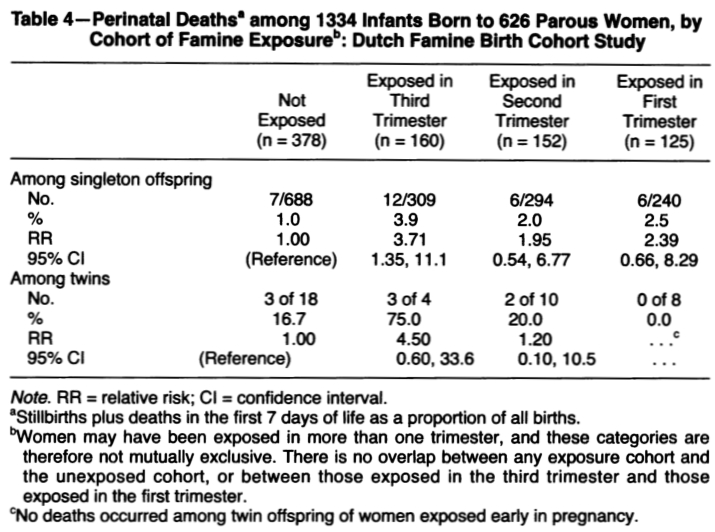
\includegraphics[width = .55\paperwidth]{ImpactEvaluation/figure/LumeySteinTable4.jpg}
}\\
\vspace*{-4.775cm}\hspace{4.5cm}\mpage{1.2cm}{
\onslide<2->{\Rect{1.2}{.3}{green}\\
}
\vspace*{-.35cm}
\onslide<4->{\Rect{1.2}{.5}{red}
}
}\\
\vspace*{-1.65cm}\hspace{3.0cm}\mpage{1.2cm}{
\onslide<2->{\Rect{1.2}{.3}{green}\\
}
}
\column{.4\paperwidth}
\onslide<3->{7/688 vs. 12/309という比較:
}
\onslide<6->{\textcolor{red}{small sample bias?}
}
\begin{dinglist}{43}
\vspace{1.0ex}\setlength{\itemsep}{1.0ex}\setlength{\baselineskip}{12pt}
\onslide<4->{\item	確かに第3三半期の方は3.82倍[表のRR=3.71は計算間違い? 下段RRは正しいが上段全て間違い]}
\onslide<5->{\item	統御群で1.02\%という珍しい症例。しかも、$310(=$全出産数688-女性総数378)件は2人目以降の出産。おそらく標本サイズが十分ではない。}
\end{dinglist}
\onslide<6->{
\begin{dinglist}{45}\footnotesize
\vspace{1.0ex}\setlength{\itemsep}{1.0ex}\setlength{\baselineskip}{12pt}
\item	例えば3\%が4.3\%に増えたとき: 誤差、それとも、43\%ポイントも増えた、と表現するのか。標本サイズ300人だと9人が13人に増えただけ。誤差。と共著者に言ったら怒られた。
\end{dinglist}
}
\end{columns}
\end{frame}

\begin{frame}{}
この標本サイズ(1病院の出生記録)で真の効果を計測できると考えない方が良い
\begin{columns}[T]
\column{.55\paperwidth}
\begin{itemize}
\vspace{1.0ex}\setlength{\itemsep}{1.0ex}\setlength{\baselineskip}{12pt}
\onslide<2->{
\item	細かなことを言えば、2人目以降の出産は選抜がある
}
\onslide<3->{
\item	1人目で正常出産すると、2人目の妊娠を望む比率は減るはず
}
\onslide<6->{
\item	だから、標本サイズはさらに小さくなる%ので、small sample biasの危険がさらに高まる
}
\end{itemize}
\column{.45\paperwidth}
\begin{itemize}
\vspace{1.0ex}\setlength{\itemsep}{1.0ex}\setlength{\baselineskip}{12pt}
\onslide<4->{
\item	2人目以降の妊娠では周産期死亡リスクがより高い人が多い標本
}
\onslide<5->{
\item	よって、1人目の妊娠だけで比較すべき
}
\end{itemize}
\end{columns}


\begin{dinglist}{43}\footnotesize
\vspace{1.0ex}\setlength{\itemsep}{1.0ex}\setlength{\baselineskip}{12pt}
\onslide<7->{
\item	最小標本サイズminimum sample size: 想定した効果と誤差の大きさの下で、一定の確率(「80\%」)で効果を検知できる最小標本サイズ。標本サイズが大きいほど誤差(サンプリング・エラー)が減って分散は小さくなり、効果を検知しやすくなる。
%の分布と効果がないときの分布を想定し、効果がある場合に(=効果あり分布から)標本を得て平均値を計算する。この平均値が80\%の確率で効果なし分布の棄却域に入ることを目指す。$n$の最小数。
%効果無しのときの分布(分散)、効果サイズeffect sizeを想定する。効果ありのときの分布は効果なし分布よりも効果サイズ分だけ右(正の効果の場合)に位置する。効果あり分布から$n$個サンプルしたときの平均値が効果なし分布の端の部分(大抵は中央80\%以外の部分)に入るために必要な最小標本サイズ。
}
\onslide<8->{
\item	効果サイズが確率2.9\%ポイント($=\tfrac{7}{688} - \tfrac{12}{309}$)増える(それだけtreatedの分布が動く)という想定で標本を得て効果を推計し、帰無仮説(曝露ありの死亡確率=曝露無しの死亡確率=.0102)が成立する確率$p$値が5\%未満であれば棄却判断する。この作業を繰り返したときに、80\%の回数で棄却判断するための標本サイズが最小標本サイズ。計算すると370人の標本が必要。
}
\onslide<9->{
\item	第1子統御群$n_{0}=378$, 第1三半期治療群$n_{1}=160$だとサンプルサイズが小さすぎる。
}
\onslide<10->{
\item	第1子統御群$n_{0}=378$, 全三半期での治療群$n_{1}=160+152+125=437$の方が最小標本サイズを満たしやすい。しかし、三半期ごとの治療群を一緒にして異なる効果を混ぜている。
}
\end{dinglist}
\end{frame}


\begin{frame}{}
\renewcommand{\arraystretch}{}
\onslide<1->{信頼性のより高いデザイン・推計方法(DID): \\~\\
}
\onslide<2->{全ての地域のコーホート・パネル・データ
}
\begin{itemize}
\vspace{1.0ex}\setlength{\itemsep}{1.0ex}\setlength{\baselineskip}{12pt}
\onslide<3->{\item	地域: アムステルダムとその他地域生まれ
}
	\begin{dinglist}{43}
	\vspace{1.0ex}\setlength{\itemsep}{1.0ex}\setlength{\baselineskip}{12pt}
\onslide<5->{	\item	同じ誕生日の人たちを他地域で見つければ良い
}
\onslide<6->{	\item	1987年時点までに死亡している女性はいる}\onslide<7->{=より健康な女性のみが残っている}\onslide<8->{=子どもの周産期死亡率は過小推計されるはず}\onslide<9->{だが、アムステルダム標本でも生存選抜について何も対応していないので、他地域標本を加えない理由が見当たらない
}
	\end{dinglist}
\onslide<4->{\item	時期: 1944年8月-1946年4月生まれ
}
\end{itemize}
\end{frame}

\begin{frame}{}
1944年8月-1945年1月、1946年1月-4月を$ym$、このうちの各月(コーホート)を$t$と表記する。$t\in ym$は「$ym$の要素の$t$」と読む。$\Delta$は前月との差分。

\vspace{-2ex}
\mpage{\textwidth}{\footnotesize
\[
\begin{aligned}
\onslide<2->{\Delta\mbox{子ど}}&\onslide<2->{\mbox{もの周産期死亡率}=}&&\\
&
\onslide<2->{\left.
  \begin{array}{l}
  \sum\limits_{t\in ym}b_{0t}*\mbox{t生まれ}+\\
  \sum\limits_{t\in ym}b_{1t}*\mbox{アムステルダム生まれ}*\mbox{t生まれ}
  \end{array}
}
\onslide<3->{\right\}} &&\onslide<3->{\mbox{\mpagethree{4cm}{\footnotesize \textcolor{azure}{その他期間生まれ\\ の対前月変化平均値}}{c}}}\\
&
\onslide<2->{\left.
  \begin{array}{l}
  +b_{21}*\mbox{第1三半期}\\
  +b_{22}*\mbox{第2三半期}\\
  +b_{23}*\mbox{第3三半期}
  \end{array}
}
\onslide<4->{\right\}}  &&\onslide<4->{\mbox{\mpagethree{4cm}{\footnotesize \textcolor{azure}{飢餓の冬生まれ\\ の対前月変化平均値}}{c}}}\\
&
\onslide<2->{\left.
\begin{array}{l}
+b_{31}*\mbox{アムステルダム生まれ}*\mbox{第1三半期}\\
+b_{32}*\mbox{アムステルダム生まれ}*\mbox{第2三半期}\\
+b_{33}*\mbox{アムステルダム生まれ}*\mbox{第3三半期}
\end{array}
}
\onslide<5->{\right\}} &&\onslide<5->{\mbox{\mpagethree{4cm}{\footnotesize \textcolor{azure}{飢餓の冬生まれで\\ アムステルダム生まれ\\ の対前月変化平均値}}{c}}}\\
\onslide<2->{&\left.+\Delta\mbox{誤差項}}\right.&&
\end{aligned}
\]
}

\vspace{1ex}
\onslide<6->{$b_{31}, b_{32}, b_{33}$は飢餓の冬該当地と他地域とのトレンドの差を表す}\\~\\
\onslide<7->{$b_{31}, b_{32}, b_{33}$で曝露の影響が測れるための識別仮定: 飢餓の冬がなければ、全地域で死亡率トレンドは共通=トレンドに地域差なし}
\end{frame}

\begin{frame}{}
CF: 他地域の1944-45年冬のトレンド
\pause : 地域間の栄養状態格差が大きくなければ信頼性高い
\begin{dinglist}{43}
\vspace{1.0ex}\setlength{\itemsep}{1.0ex}\setlength{\baselineskip}{12pt}
\pause
\item	識別仮定そのもの(アムステルダム1944-45年冬のCF=他地域1944-45年冬の変化分)はCFが観察できないので検定できない
\pause
\item	しかし、それ以外の時期で成り立っていれば、1944-45年冬にも成り立つ蓋然性が高い
\end{dinglist}
\pause
\vspace{2ex}
$b_{1t}=0$を$t$すべてについて検定すれば、1944-45年冬以外でアムステルダムとその他地域で共通トレンドの有無を確認できる
\pause
\begin{dinglist}{45}
\vspace{1.0ex}\setlength{\itemsep}{1.0ex}\setlength{\baselineskip}{12pt}
\item	より望ましくは...\pause
成人1人当たり配給カロリー(飢餓の冬は1000カロリー/日)を全標本から得られれば、推計式に各期各地域の配給カロリーを加えると、周産期死亡率とコーホート、周産期死亡率と配給カロリーの関係を分離して計測でき、\textcolor{red}{配給カロリーが影響しているか}確認できる
\end{dinglist}
\vspace{2ex}
\pause
自然実験は個人ごとに実際の「治療」が観察できないので、生まれた時期と地域で曝露を仮定せざるを得ない\\
\pause
\vspace{1ex}
{\footnotesize 仮説の原因(栄養不足)とより近接した配給カロリーを用いる方が検定結果解釈の確度は増す}
\end{frame}

\begin{frame}{Regression discontinuity design}
全ての特徴を観察できれば結果の差をすべて説明できる。が、観察できない。\\
\pause
実験でなく、パネル・データが(=DIDができ)ないとき、どうすれば良いのか?\\~\\
\pause
Good news: \pause インパクト評価の範囲を狭くすれば、推計可能。
%There is, if we limit our attention to a narrower domain.
\\~\\

\pause
Consider a poverty reduction policy that gives a subsidy to the people below the poverty line.
\begin{dinglist}{45}
\vspace{1.0ex}\setlength{\itemsep}{1.0ex}\setlength{\baselineskip}{12pt}
\pause
\item	 ``BPL'' card in India.
\end{dinglist}
\pause
\vspace{2.0ex}
Suppose poverty line is USD 1.25 per day and this criteria is strictly enforced. So if your income is USD 1.24 per day, you get the money. If your income is USD 1.25, you don't.\\~\\

\pause
People with daily income of USD 1.24 and USD 1.25 are similar. \\~\\

\pause
Estimate impacts by comparing BPL and APL near the poverty line.
\end{frame}

\begin{frame}{}
The narrower focus around cutoff gives us a ``matched pair'' or forms a counterfactual. \\~\\
\pause

Interpretation of estimates: Policy impacts on the subpopulation near the cutoff. \pause 
It is a local impact we are estimating, not a global impact such as ATE (and ATT, ATC). \\~\\

\pause
Applications: Cutoffs, geographical boundaries.\\~\\

\pause
Policies are full of cutoffs. So almost every policy has a chance of estimating its impacts near the cutoff.\\~\\

\pause
Identifying assumption:
\pause
There is nothing other than policy cutoff that has a discrete jump around the cutoff point. So a jump in the outcome can be attributed only to the policy.\\~\\

\pause
But there is a catch: (Because we fit the line locally around the cutoff neighbourhood) It takes a large sample to use RDD estimator with the order of 10,000. 
\end{frame}

\begin{frame}{}
因果関係を示す方法: \textbf{回帰不連続regression discontinuity design (RDD)}\\~\\
\pause
右辺の変数が急に変化する状況を見つけ、その前後で左辺の変化を観察する\\~\\
\pause
teacher-pupil ratio $\Rightarrow$ exam score\\~\\
\pause
メモニデス(中世のトーラー学者)による戒律\\
\pause
``Only up to 40 students in one class....''\\
\pause
\hfil\visible<6>{\includegraphics[width = 6cm]{ImpactEvaluation/figure/maimonides-mishna.eps}}
\end{frame}

\begin{frame}{}
\hfil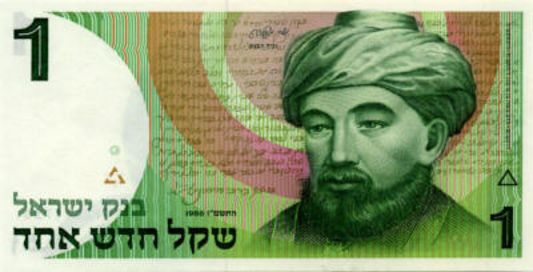
\includegraphics[width = 12cm]{ImpactEvaluation/figure/maimonides.eps}
\end{frame}

\begin{frame}{}
The Government of Israel still holds it. \\
\pause
\hfil\visible<2>{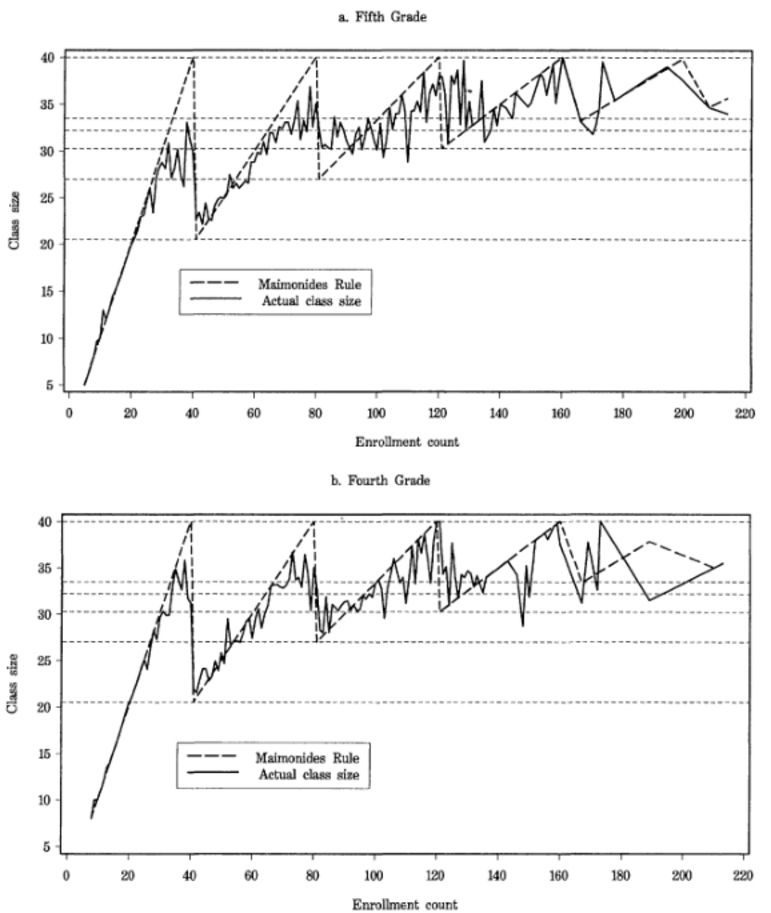
\includegraphics[height = 8cm]{ImpactEvaluation/figure/AEvans_Fig01.eps}}\\
\end{frame}

\begin{frame}{}
Ingenuity of \citet{AngristLavy1999}: Predicited class size vs. exam scores.\\
\mpage{14cm}{\mpagethree{10cm}{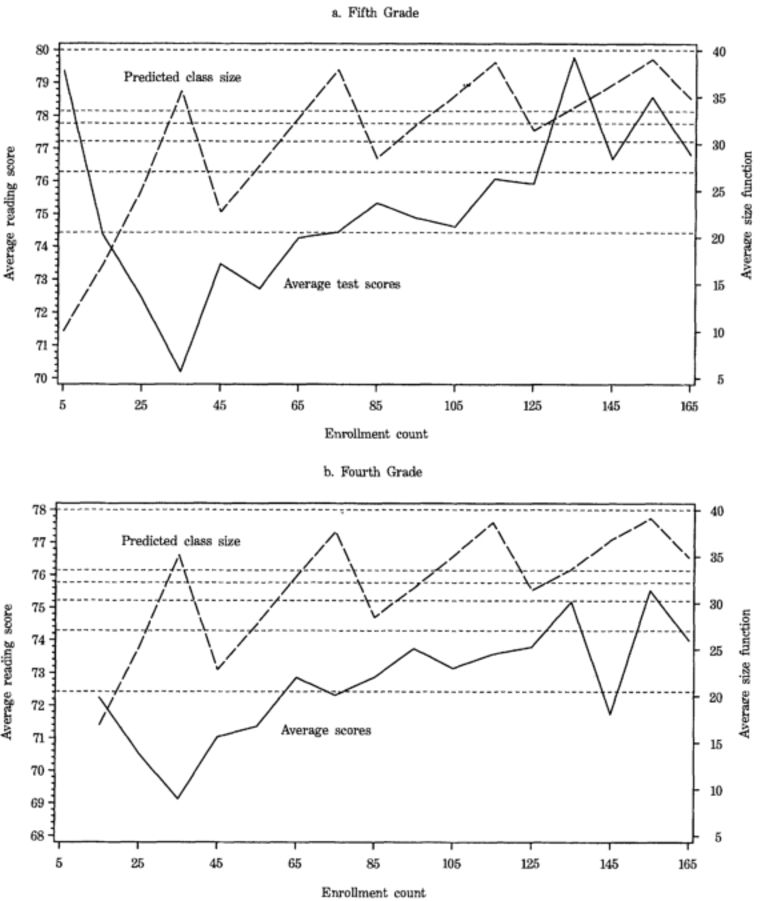
\includegraphics[height = 8cm]{ImpactEvaluation/figure/AEvans_Fig02.eps}}{c}\hspace{-3cm}\mpagethree{4.5cm}{Impact is more evident in smaller enrollment counts. Average score is increasing after 60 regardless of predicted class size. Possible reasons: Greater deviation of actual class size from predicted class size, different petagogical methods in large schools or more competition/learning among peers.}{c}}
\end{frame}

\begin{frame}[t]{}
4th graders\\
\hfil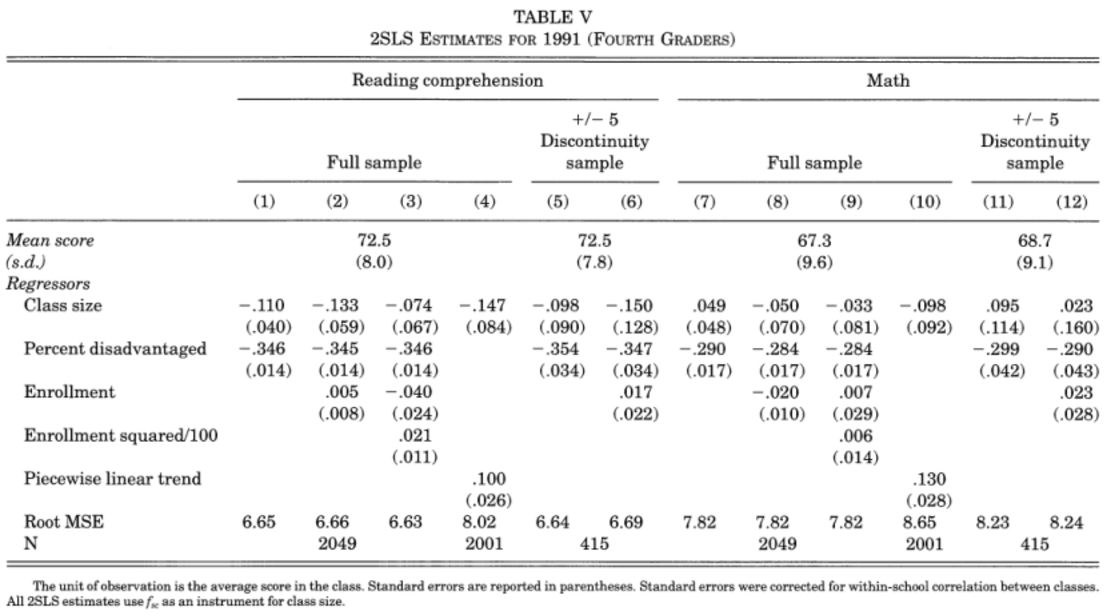
\includegraphics[width = 11cm]{ImpactEvaluation/figure/AEvans_Tab05.eps}\\
Using all sample, there is a negative relationship between class size and learning only in reading but not in maths. For 4th graders, no impacts of class size at discontinuity neighbourhood sample.\\
\vspace{-4.9cm}\hspace{3.4cm}\Rect{1.5}{.5}{red}
\end{frame}

\begin{frame}[t]{}
4th and 5th graders\\
\hfil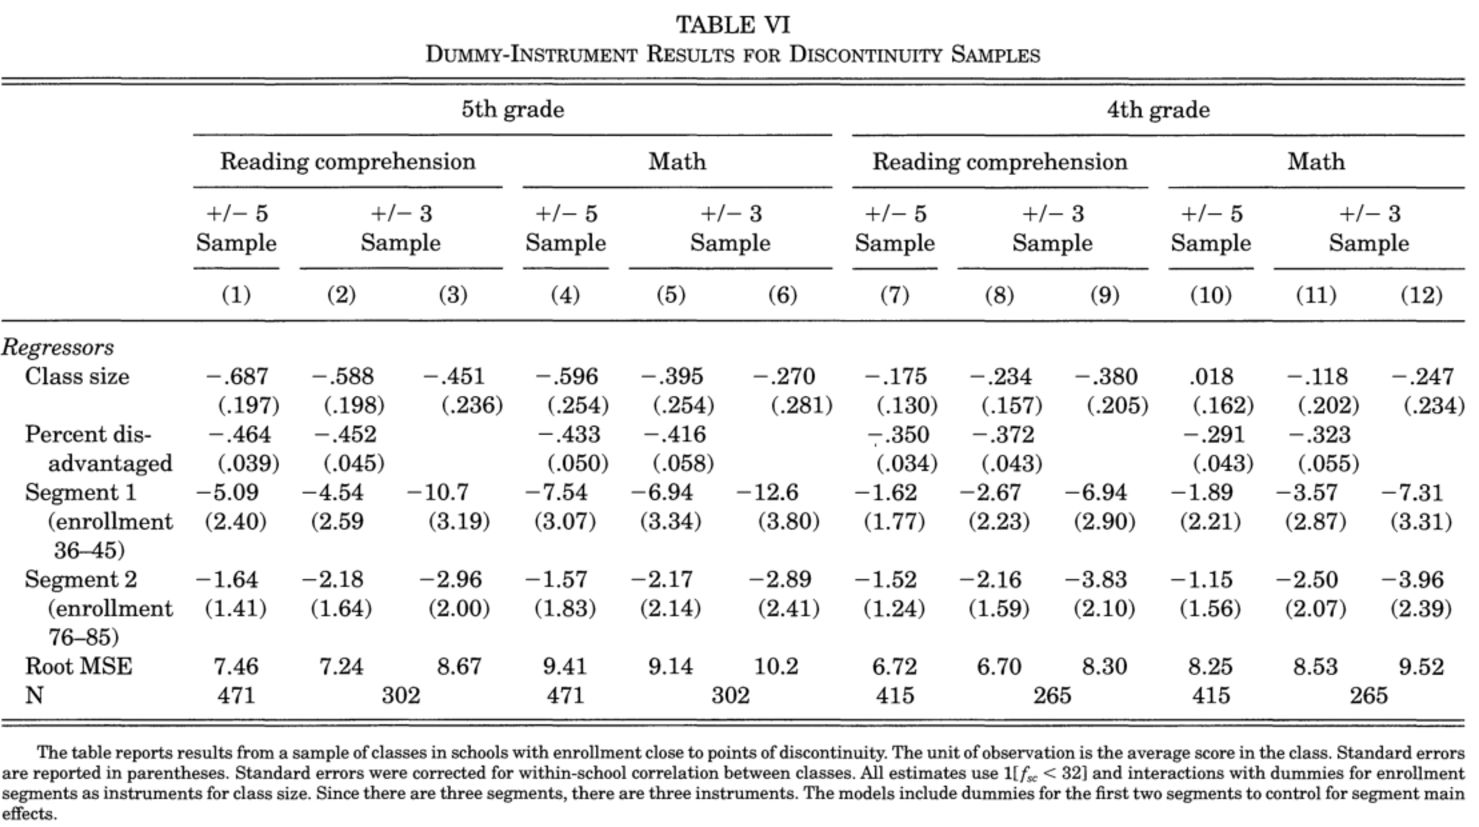
\includegraphics[width = 11cm]{ImpactEvaluation/figure/ALavy_Tab06.eps}\\
For 5th graders, using discontinuity neighbourhood sample, there is a negative causal relationship between class size and learning in both reading and maths.\\
\vspace{-4.7cm}\hspace{2.5cm}\Rect{2.6}{.5}{red}\hspace{-.1cm}\Rect{.7}{.5}{red}
\end{frame}


\begin{frame}{}
横浜市2009年40人学級: 小6国語(共通試験点数偏差値)\\
\hfil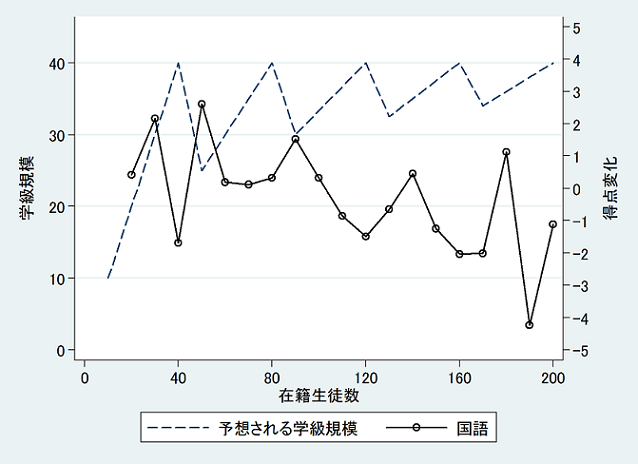
\includegraphics[width = 11cm]{ImpactEvaluation/figure/Akabayashi_ClassSizeYokohamaShou6.png}\\
\citet{Akabayashi2013}
\end{frame}

\begin{frame}{}
横浜市2009年40人学級: 中3国語(共通試験点数偏差値)\\
\hfil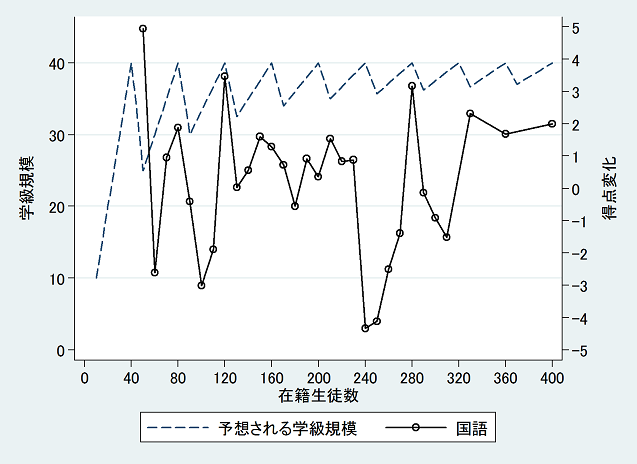
\includegraphics[width = 11cm]{ImpactEvaluation/figure/Akabayashi_ClassSizeYokohamaChu3.png}\\
\citet{Akabayashi2013}
\end{frame}

\begin{frame}{}
赤林さんは中3国語で期待した成果が出なかったことに驚くが、以下のように解釈 {\footnotesize \url{https://synodos.jp/education/12530}}\\~\\
\pause
少人数学級=きめ細やかな指導が可能、なので、自動的に成績が上がるわけではない\\~\\
\pause
教員の指導能力、意欲、効率性重視方針も必要\\~\\
\pause
教員の数が増えれば能力が低い、意欲が弱い人も雇用される\\~\\
\pause
伸び代が高い生徒に注力(効率性重視)するか、成績の低い生徒に注力(公平性重視)するか\\~\\
\pause
どうも地価の高い地域では成績が上がったようです(論文アクセスないので未読)\\~\\
\pause
情報開示請求で得た学校平均点数と学年生徒数のデータなので、実際のクラス数(よって、実際のクラス・サイズ)は分からない模様\\~\\
\pause
点数がより変化しやすそうな英語や数学の結果が知りたい
\end{frame}

\begin{frame}{}
中室牧子さん: 35人学級は、2011年に公立小学校の1年生に対してのみ導入されました。財務省は、2011年以前と以後で、いじめ、暴力行為、不登校の平均値を比べると、いじめや暴力、不登校には大きな変化が見られないので、少人数学級には効果がない。したがって、「40人学級に戻すべき」と主張したのです。\\~\\
\hfil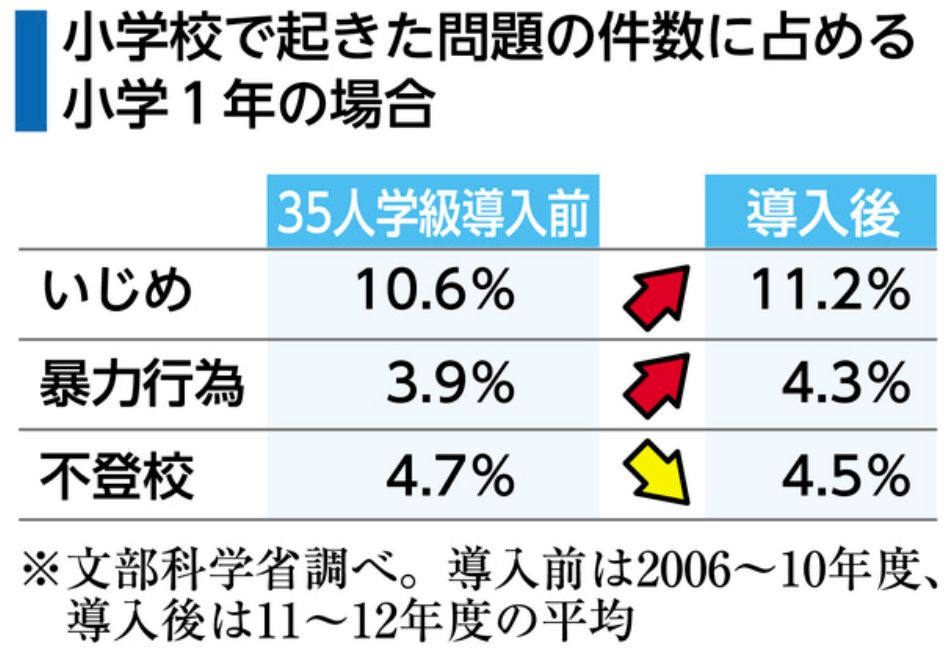
\includegraphics[height = 4cm]{ImpactEvaluation/figure/35ninGakkyu_DiamondOnline.jpg}\\
\url{https://diamond.jp/articles/-/66992}\\~\\

\pause
この効果推計で不適切な点: 帰無仮説(効果ゼロ)の$p$値がない、推計方法(識別仮定)の信頼性が低い、プラシーボ検定(私立1年生や公立2年生)もできる
\end{frame}

\begin{frame}{}
日経新聞2020年12月17日(木)朝刊\\
\hfil\mpagethree{5cm}{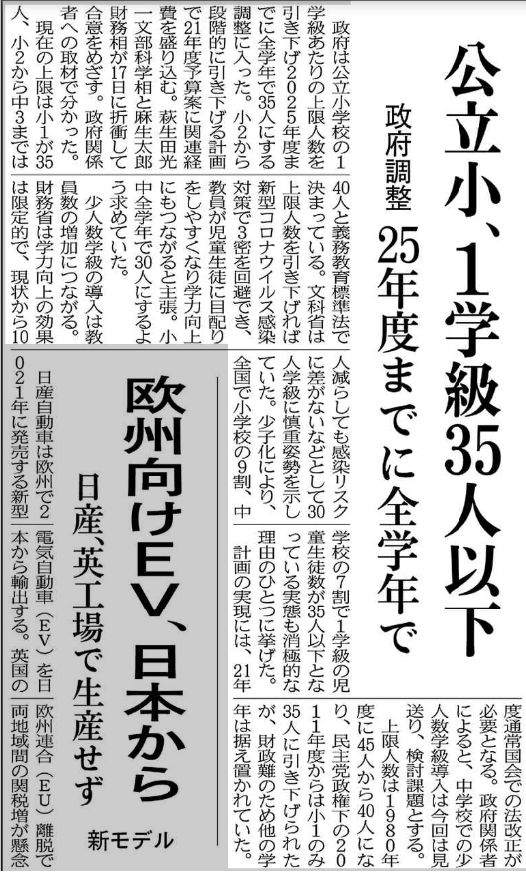
\includegraphics[width = 5cm]{ImpactEvaluation/figure/Nikkei_35NinClass2020Dec17.jpg}}{c}
\mpagethree{6cm}{3密回避が動機\\~\\
今回も(35人が良いとする)エビデンスに依拠せず\\~\\
全国一律だと効果推計は難しい}{c}
\end{frame}

\begin{frame}{}
\begin{itemize}
\vspace{1.0ex}\setlength{\itemsep}{1.0ex}\setlength{\baselineskip}{12pt}
\item	\citet{LemieuxMilligan2008}: In Quebec, unemployment benefits are increased once reaching the age of 30 for adults with no child. This should have disincentives to work for age 30 and older. If this is true, at around 30, work outcomes will be reduced.
	\begin{dinglist}{43}
	\vspace{1.0ex}\setlength{\itemsep}{1.0ex}\setlength{\baselineskip}{12pt}
\pause
	\item	Will there be a jump in employment rates at 30 to the below?
	\end{dinglist}
\pause
\item	\citet{Lee2008}: Being an incumbent can give an additional benefit in the next election. If this is true, at the vote share margin close to zero, an incumbent vs. non-incumbent contrast gives effects of this benefit. Most suitable data comes from the US state gubernatorial elections where there are effectively only two candidates/parties.
	\begin{dinglist}{43}
	\vspace{1.0ex}\setlength{\itemsep}{1.0ex}\setlength{\baselineskip}{12pt}
\pause
	\item	Will there be a jump in winning probability at zero vote margin to the above?
	\end{dinglist}
\end{itemize}
\end{frame}

\begin{frame}{}
\citet{LemieuxMilligan2008}. Age and unemployment benefits in Quebec.\\
\hfil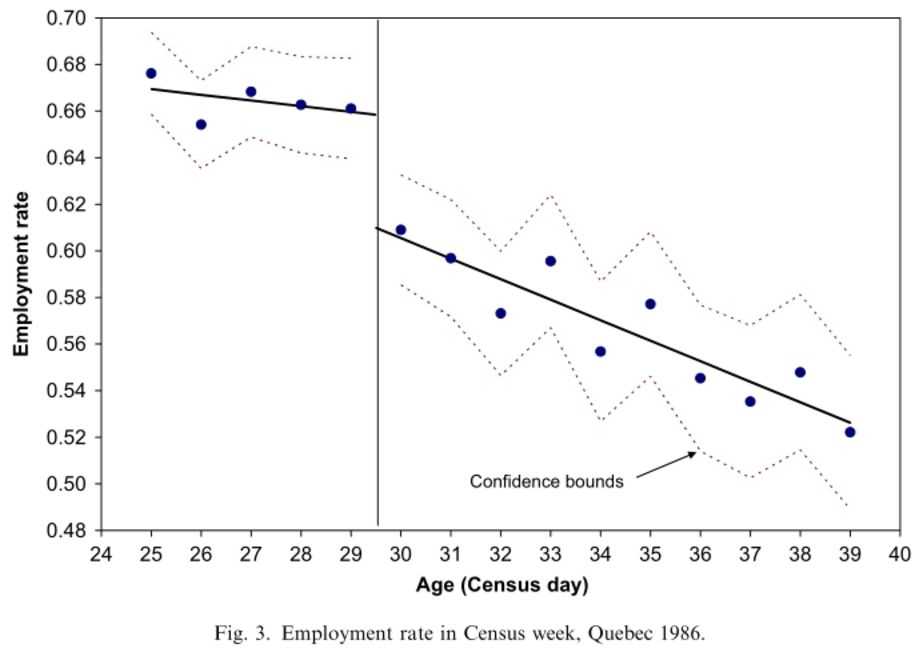
\includegraphics[height = 8cm]{ImpactEvaluation/figure/Lemieux_Fig03.eps}
\end{frame}
\begin{frame}{}
\citet{Lee2008}. Margin of vote share in $t$ and probability of winning in $t+1$.\\
\hfil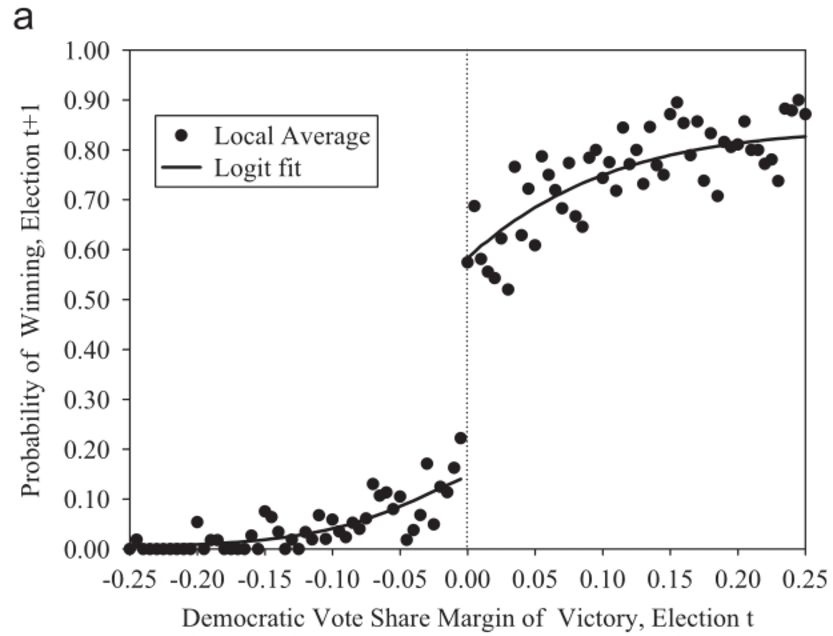
\includegraphics[height = 8cm]{ImpactEvaluation/figure/Lee_Fig02a.eps}
\end{frame}


\begin{frame}{}
There is an indirect yet nice use of data to assess the logical coherence of the results.\\~\\

\pause
Take a sample that should not be affected by the policy and test if there is an impact. \\~\\

\pause
If there is an impact, then your main result is likely to be also picking up something different from the policy.\\~\\

\pause
This is called a \textit{placebo test}.\\~\\

\pause
A placebo test is run only when the main estimation indicates a non-zero effect.\\~\\

\pause
If the main estimate has a low $p$ value (probability of null hypothesis `zero effect' being true), one tries to run a placebo test, in a hope of finding a large $p$ value in it, to get a further confidence that the result is not an accident.
\end{frame}

\begin{frame}[t]{}
Placebo tests in \citet{LemieuxMilligan2008}. Rest of Canada or post 1991 should not detect effects.\\
\hfil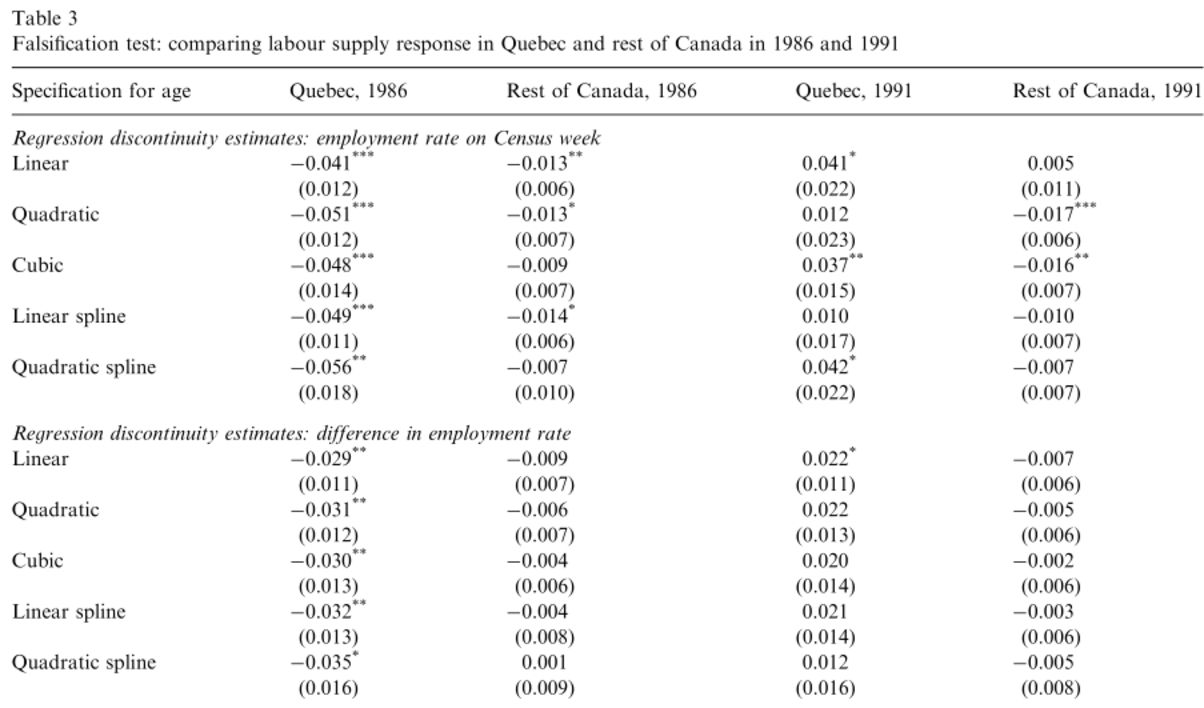
\includegraphics[height = 7cm]{ImpactEvaluation/figure/Lemieux_Tab03.eps}\\
\vspace{-5.65cm}\hspace{3.5cm}\Rect{1.25}{.5}{blue}\hspace{.9cm}\Rect{3.6}{.55}{red}\\
\vspace{2.3cm}\hspace{3.5cm}\Rect{1.25}{.5}{red}\hspace{.9cm}\Rect{3.6}{.55}{red}
\end{frame}

\begin{frame}{}
Placebo tests in \citet{Lee2008}. Margin of vote share in $t$ should not give a jump of events before $t$.\\
\hfil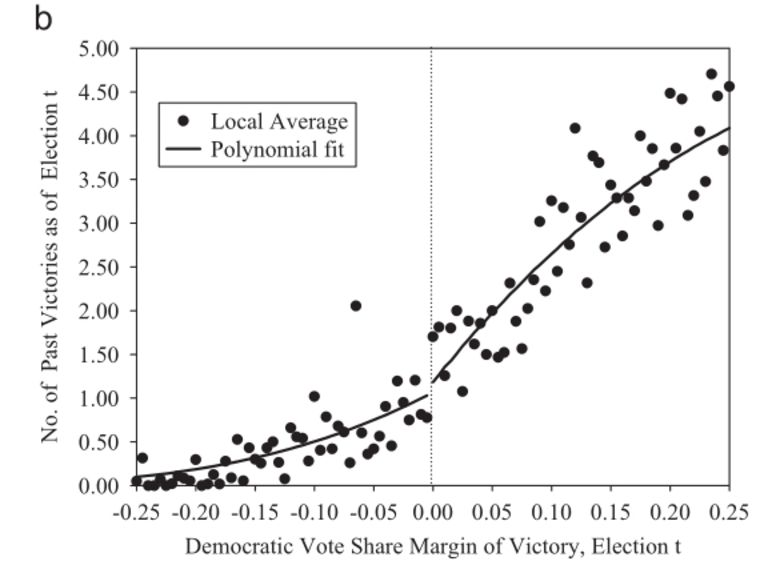
\includegraphics[height = 8cm]{ImpactEvaluation/figure/Lee_Fig02b.eps}
\end{frame}

\begin{frame}{}
現在ではカットオフから遠い標本を使った多項式(曲線)をフィットさせることは誤りとされている\\~\\
\begin{dinglist}{45}
\vspace{1.0ex}\setlength{\itemsep}{1.0ex}\setlength{\baselineskip}{12pt}
\item	カットオフから遠い標本は推計に重用されるべきではない
\item	多項式はカットオフから遠い標本の僅かな値の変動によって推計値が大きく変化する
\end{dinglist}

\vspace*{2ex}
現在は直線、もしくは、local linear regressionという遠い標本のウェイトを小さくして直線を推計する手法を使う
\end{frame}

\begin{frame}{}
When applied to geographical boundaries, such as school zones, there may be parents who move across border for better education.\\~\\

\pause
Then the cutoff becomes nondeterministic, or ``fuzzy.'' If the jump does not happen exactly at the predetermined cutoff, RDD is said to have a \textit{fuzzy design}. 
\begin{dinglist}{43}
\vspace{1.0ex}\setlength{\itemsep}{1.0ex}\setlength{\baselineskip}{12pt}
\pause
\item	There can be many instances of fuzzy RDD if one can fabricate the eligibility. In India's BPL example, the BPL card can be issued to a resident who pays a bribe. This introduces a noise in estimates, hence estimates become less precise.
\pause
\item	Nonetheless, a fuzzy RDD can also give a consistent estimate of local impacts, as long as we have a large enough sample that complies with the cutoff.
\end{dinglist}

\pause
If there is not cross cutoff movement, RDD is said to have a \textit{sharp design}.
\end{frame}

\begin{frame}{}
RDDは局地的な実験と捉えられる\\~\\
境界内外で越境があったとしても、treatment assignmentについて人々の意向が不正確にしか反映されなければ、ランダムな割当の要素があるから\\~\\
実験と同様、density testはランダム化を達成できたか検定
\end{frame}


\begin{frame}{}
RDD	での識別仮定の信頼性チェック
\begin{description}
\vspace{1.0ex}\setlength{\itemsep}{1.0ex}\setlength{\baselineskip}{12pt}
\pause
\item[placebo test]	欠落変数の影響を確認: 政策変化のない点の推計値がゼロを検定\pause
...棄却 $\Rightarrow$ 推計した効果に疑問
\pause
\item[density test]	非越境(local randomisation)の確認: 
	\begin{itemize}
	\vspace{1.0ex}\setlength{\itemsep}{1.0ex}\setlength{\baselineskip}{12pt}
\pause
	\item	越境者が多ければ境界で標本が多くなり、分布に凹凸ができる: forcing variableの分布密度が境界内外で等しい(=帰無仮説: 越境がなく分布の差が境界内外でゼロ)か検定(density test or McCary test)\pause
...棄却 $\Rightarrow$ 越境あり 
\pause
	\item	治療確率(propensity scoreという)の差が境界内外でゼロ(=帰無仮説: 越境が完全で治療確率に対し境界が無意味になる)か検定\pause
...棄却 $\Rightarrow$ 越境なし
\pause
	\item	特定の特徴を持つ人たちが越境していないか: その他変数の平均値が境界内外で等しい(=帰無仮説: 越境がなく平均値の差が境界内外でゼロ)か検定\pause
...棄却 $\Rightarrow$ 越境あり
	\end{itemize}
\end{description}
\vspace*{2ex}
\pause
PTは論理的なチェックで傍証。DTはランダム化の検定。
\end{frame}


\begin{frame}{}
fuzzy designの(越境者がいる)場合: propensity scoreが0と1ではなく$p_{0}, p_{1}\in(0,1), p_{0}<p_{1}$の場合\\~\\

\pause
確率差$p_{1}-p_{0}$でカットオフでの平均値差$\bar{y}_{1+}-\bar{y}_{0-}$を補正\\~\\
\pause
\[
\mbox{カットオフ近辺での効果}=\frac{\bar{y}_{1+}-\bar{y}_{0-}}{p_{1}-p_{0}}.
\]
\pause
sharp designだったら$p_{1}=1, p_{0}=0$
\begin{dinglist}{43}
\vspace{1.0ex}\setlength{\itemsep}{1.0ex}\setlength{\baselineskip}{12pt}
\pause
\item	exclusionのみがあるとき($p_{0}=0, p_{1}<1$): 計測される平均値差$\bar{y}_{1+}-\bar{y}_{0-}$は真の効果$\alpha$の$100*p_{1}\%$ \pause
$\rightarrow$ $\alpha=\frac{\bar{y}_{1+}-\bar{y}_{0-}}{p_{1}}$
\pause
\item	leakageのみがあるとき($p_{0}>0, p_{1}=1$): 計測される平均値差$\bar{y}_{1+}-\bar{y}_{0-}$は$\alpha-p_{0}\alpha$\pause
 $\rightarrow$ $\alpha=\frac{\bar{y}_{1+}-\bar{y}_{0-}}{1-p_{0}}$
\pause
\item	exclusionとleakageがあるとき($p_{0}>0, p_{1}<1$): 計測される平均値差$\bar{y}_{1+}-\bar{y}_{0-}$は$p_{1}\alpha-p_{0}\alpha$\pause
 $\rightarrow$ $\alpha=\frac{\bar{y}_{1+}-\bar{y}_{0-}}{p_{1}-p_{0}}$
\end{dinglist}
\end{frame}

\begin{frame}{}
\citet[][Figure 2]{BoschSchady2019}: density testの例\\
\hfil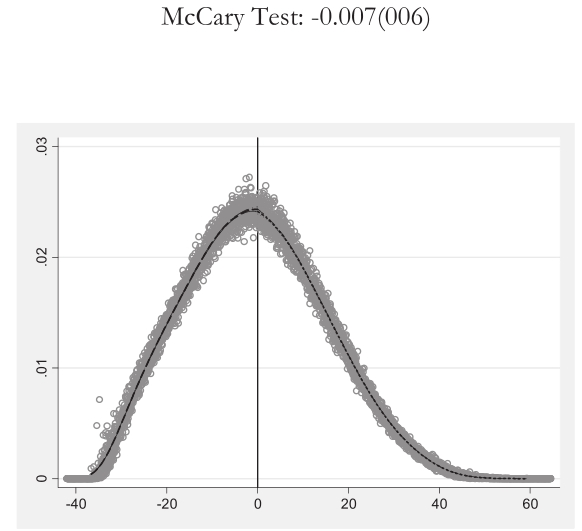
\includegraphics[height = 7cm]{ImpactEvaluation/figure/BoschSchady_DensityTest.jpg}\\
\vspace*{2ex}
確率密度は境界でジャンプしていないことが視覚的に分かる(検定結果の統計値は-.007、標準誤差が.006)
\end{frame}

\begin{frame}{}
\citet{DufloDupasKremer2011}: 習熟度別学級実験(ケニア)\\~\\
\pause
2005年2学期-2006年学年終了、ケニア西部、1年生が単一学級の小学校121校
\begin{description}
\vspace{1.0ex}\setlength{\itemsep}{1.0ex}\setlength{\baselineskip}{12pt}
\pause
\item[統御群]	61校: 単一学級$\rightarrow$2つの学級(契約教員1名を雇用)、生徒の割り振りはランダム
\pause
\item[治療群]	60校: 単一学級$\rightarrow$2つの習熟度学級(契約教員1名を雇用)、1学期試験点数で割り振り(成績百分位50\%がカットオフ)、契約教員と正規教員を習熟度学級についてランダムに配置
\end{description}
\pause
\vspace*{1ex}
ランダム化\\
\pause
tracking schools: 習熟度学級有無$*$教員雇用形態\\
\pause
nontracking schools: 級友(peer)の成績$*$教員雇用形態
\end{frame}

\begin{frame}{}
習熟度学級の学校は平均点数が分かれる=実験は概ね正しく実施\\
\hfil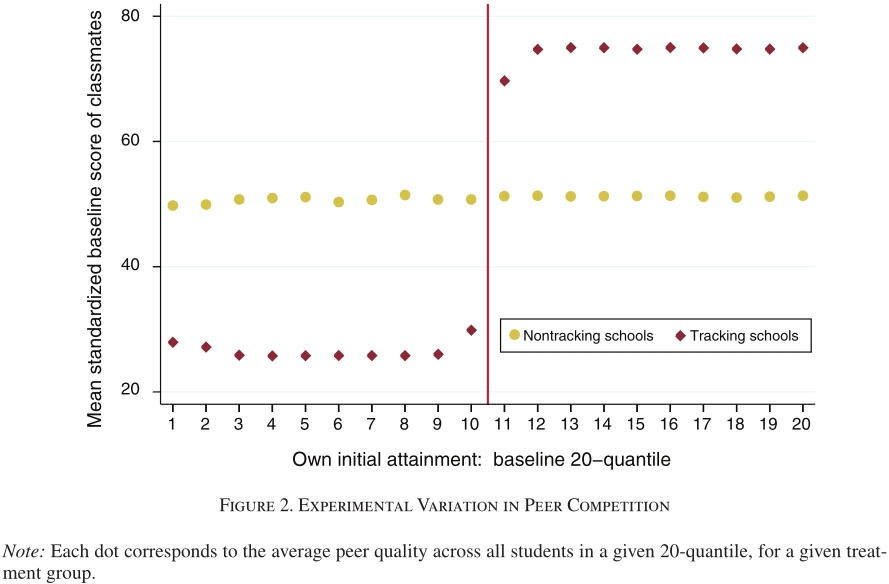
\includegraphics[height = 8cm]{ImpactEvaluation/figure/DufloDupasKremer_KenyaTrackingPeerEffectFigure2.jpg}
\end{frame}
\begin{frame}{}
Local linear regression: 境界(50)点で2006年試験点数に変化なし\\
\hfil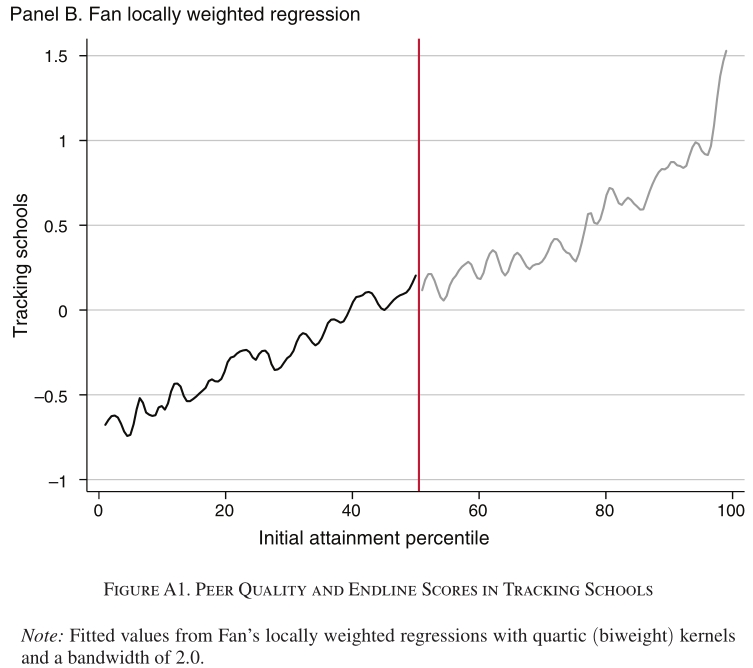
\includegraphics[height = 8cm]{ImpactEvaluation/figure/DufloDupasKremer_KenyaTrackingPeerEffectFigureA1PanelB.jpg}
\end{frame}
\begin{frame}{}
Local averageとglobal quadratic (2次関数、なぜやったのか不明)\\
\hfil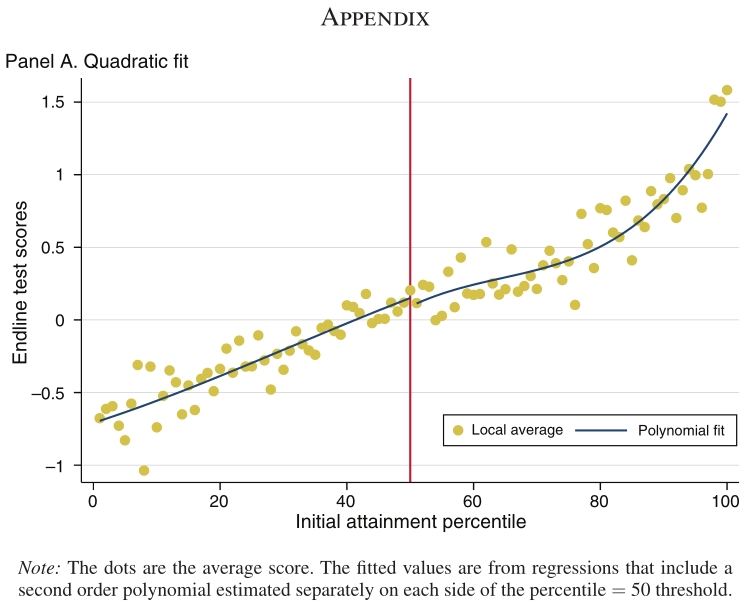
\includegraphics[height = 8cm]{ImpactEvaluation/figure/DufloDupasKremer_KenyaTrackingPeerEffectFigureA1PanelA.jpg}
\end{frame}
\begin{frame}{}
習熟度学級の学校は分布全体で2006年末試験点数が上がる\\
\hfil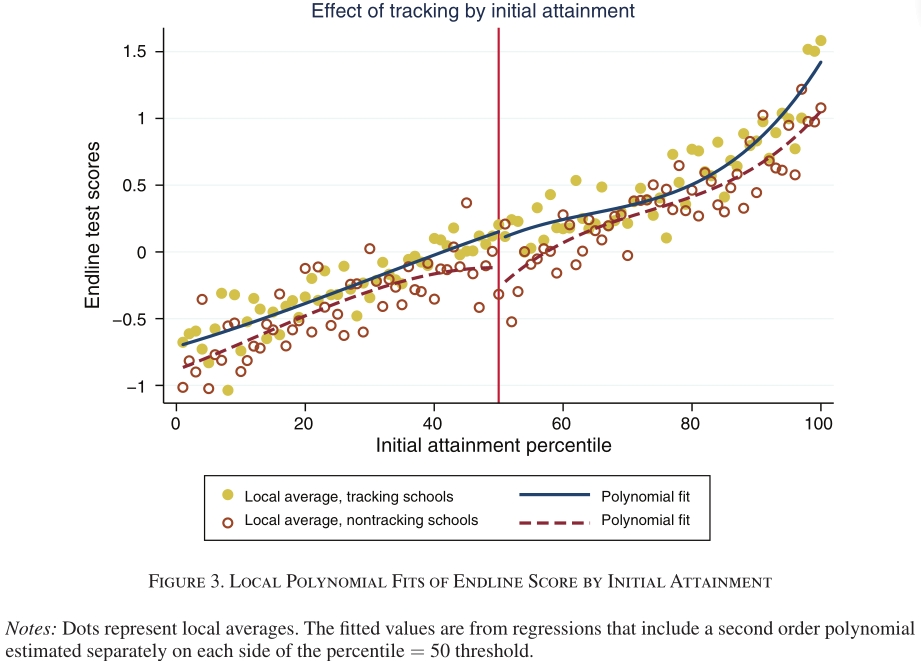
\includegraphics[height = 7cm]{ImpactEvaluation/figure/DufloDupasKremer_KenyaTrackingPeerEffectFigure3.jpg}\\
``local polynomial fits''は、注から類推するとおそらく2次関数なので信頼性はあり、位置は上に来そうだが各点での検定(nontrackingとの差がゼロ)の$p$値は示されていない
\end{frame}

\setbeamercovered{invisible}
\begin{frame}[t]{}
\begin{columns}[T]
\column{.7\paperwidth}
\onslide<1->{\hfil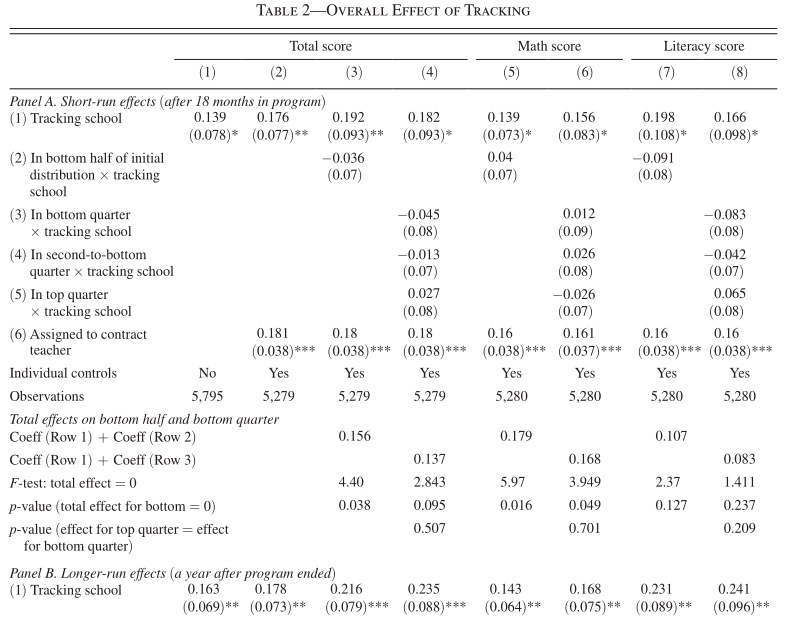
\includegraphics[height = 8cm]{ImpactEvaluation/figure/DufloDupasKremer_KenyaTrackingPeerEffectTable2.jpg}\\
}
\column{.25\paperwidth}
\onslide<2->{全体の平均値の差がゼロという帰無仮説の$p$値\\~\\}
\onslide<3->{2006年末: 10\%以下}\\
\onslide<4->{2007年末: 5\%以下\\}
\end{columns}

\vspace*{-6.7cm}\mpage{\paperwidth}{
\onslide<3->{\hspace{2.35cm}\Rect{7.75}{.5}{red}\\}

\vspace*{5cm}\noindent
\onslide<4->{\hspace{2.35cm}\Rect{7.75}{.5}{red}}
}
\end{frame}

\begin{frame}[t]{}
\begin{columns}[T]
\column{.7\paperwidth}
\hfil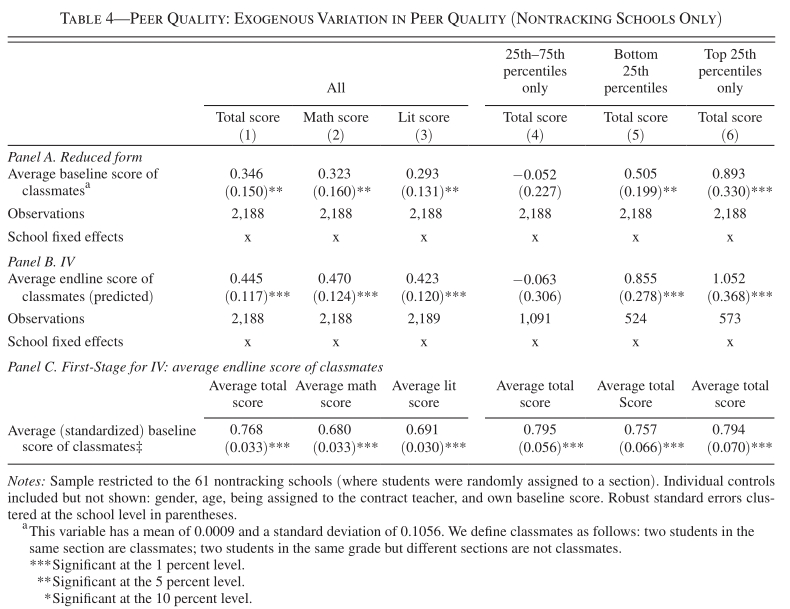
\includegraphics[height = 8cm]{ImpactEvaluation/figure/DufloDupasKremer_KenyaTrackingPeerEffectTable4.jpg}
\column{.25\paperwidth}
\onslide<2->{
Nontracking学校はpeer efffectsが平均的に正\\~\\
}
\onslide<3->{
とくに下位と上位の生徒において正\\~\\
}
\onslide<4->{
下位が正なのは想像に難くないが、上位が正なのは解釈が複雑
}
\end{columns}

\vspace*{-5.9cm}
\mpage{\paperwidth}{\onslide<2->{
\hspace{2.85cm}\Rect{3.25}{.5}{red}}\onslide<3->{\hspace{1.7cm}\Rect{2.2}{.5}{red}}\\
}
\end{frame}

\begin{frame}{}
学区と成績と地価\citep{Black1999, BayerFerreiraMcMillan2007}\\~\\
\begin{columns}[T]
\column{.5\paperwidth}
\hfil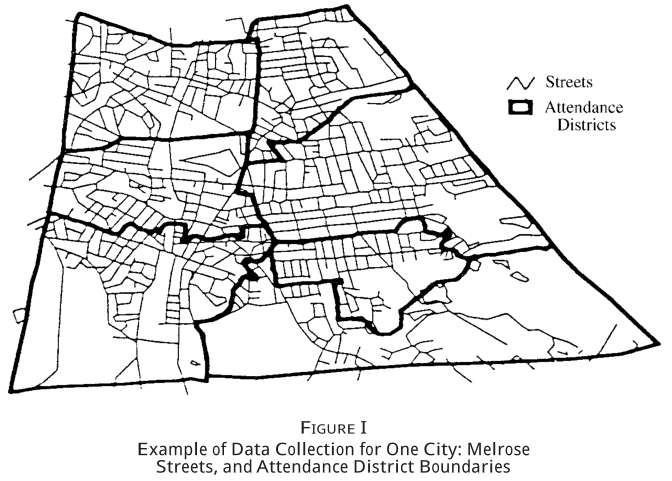
\includegraphics[height = 5cm]{ImpactEvaluation/figure/Black_SchoolDistricts.jpg}\\
\column{.45\paperwidth}
\pause
学区境界を挟んだ家計グループを比較\\~\\
\pause
forcing variable=(垂直距離で)最も近い境界までの距離\\~\\
\pause
outcome variables=試験点数、不動産価格
\end{columns}
\pause
\citet{Black1999}: 不動産価格(不動産取引データ)、学区と各校試験点数(MEAP)、その他変数(センサス)\\
\pause
\citet{BayerFerreiraMcMillan2007}: 不動産価格と試験点数(センサス)、不動産価格(不動産取引データ)、その他変数(センサス)
\end{frame}

\begin{frame}{}
学区や学校単位での比較\\~\\
\pause
観察できない学区間の違い(欠落変数omitted variable、親の知的能力、家庭の躾、教員の質や熱意、教授法の違い、学級崩壊度、治安、騒音、環境汚染など)が結果に影響を与えている可能性あり\\~\\
\pause
学区境界を挟んだ狭い地域同士の比較\\~\\
\pause
学区境界に共通する観察できない変数の一部は同じと想定できる\\
\pause
$\Rightarrow$ 結果の差の一部は学区の違い(のはず)
\begin{dinglist}{45}
\vspace{1.0ex}\setlength{\itemsep}{1.0ex}\setlength{\baselineskip}{12pt}
\pause
\item	学区境界のどちら側かがランダムと考えることはできない
\pause
...親は学区を気にして家を買う・借りる
\pause
\item	親の能力や資産などが同じとは思えない
\pause
...しかし、観察可能な変数(学歴や所得など)はPT、DTで検定可能
\pause
\item	川、公園、ゴルフ場境界などで区切られた境界だと、境界内外で観察できない変数は同じと思えないので標本から除外
\pause
\item	少なくとも家庭の外部環境要因(治安、騒音、公害など)は揃えて推計する
\pause
...学区ごとの比較よりもまし
\end{dinglist}
\end{frame}

\begin{frame}{}
\vspace*{-4.0cm}

\mpage{14cm}{\onslide<1->{\mpagethree{7cm}{\hfil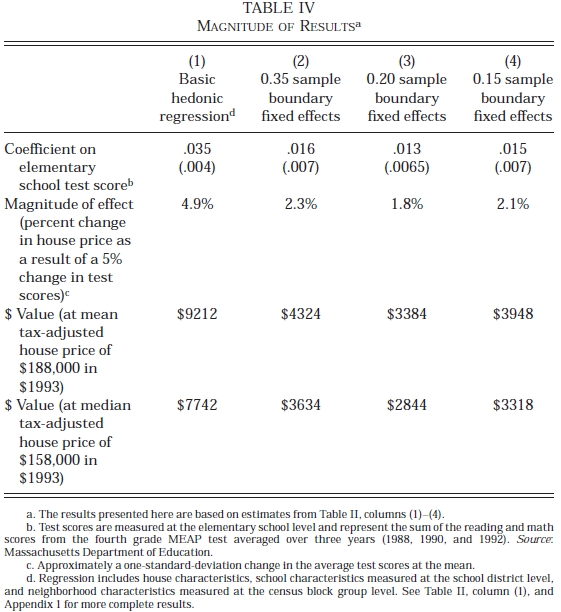
\includegraphics[height = 8cm]{ImpactEvaluation/figure/Black_SchoolDistricts_MagnitudeTable.jpg}\\

\vspace*{-6.1cm}\hspace{3.4cm}\Rect{3.5}{.5}{red}
}{c}} \hspace{1em}\mpagethree{4cm}{
\vspace*{3cm}
\onslide<2->{境界を挟んだ比較は学区間比較4.9\%よりも地価に与える効果は小さい\\~\\}
\noindent
\onslide<3->{観察できない変数を揃えると地価に与える影響は半分以下(2.3, 1.8, 2.1)になる\\~\\}
\noindent
\onslide<4->{$\Rightarrow$}\onslide<5->{学区間比較での効果: 観察できない変数の効果が半分以上}
}{c}
}
\end{frame}

\begin{frame}{}
\citet{BayerFerreiraMcMillan2007}: 左列はセンサス(回答者情報)データ、右列は不動産取引データ\\
\hfil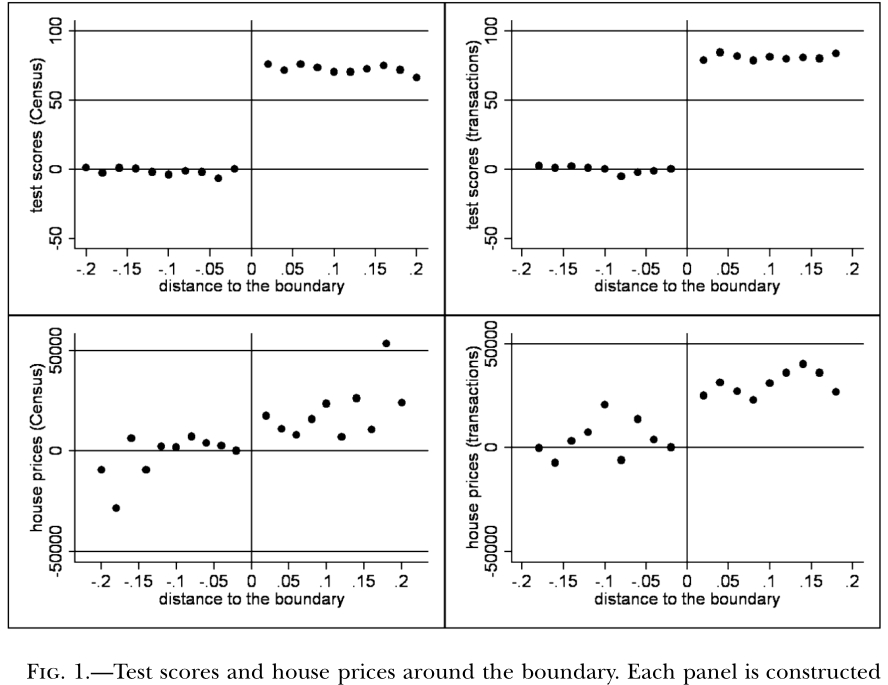
\includegraphics[height = 8cm]{ImpactEvaluation/figure/Bayer_Fig1.jpg}\\
\end{frame}
\begin{frame}{}
\citet{BayerFerreiraMcMillan2007}: 物件の特徴は境界内外で連続\\
\hfil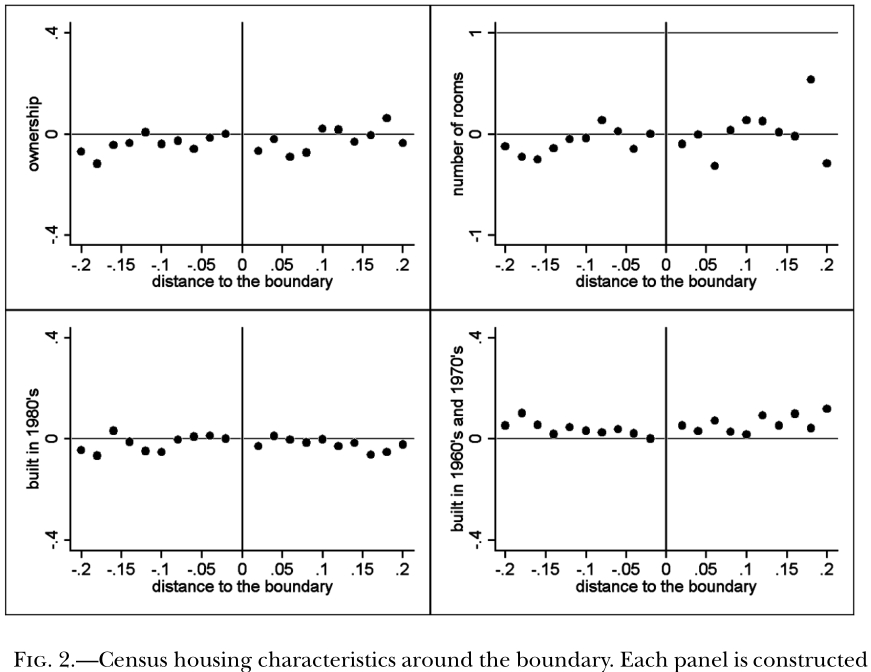
\includegraphics[height = 8cm]{ImpactEvaluation/figure/Bayer_Fig2.jpg}\\
\end{frame}
\begin{frame}{}
\citet{BayerFerreiraMcMillan2007}: 物件の特徴は境界内外で連続\\
\hfil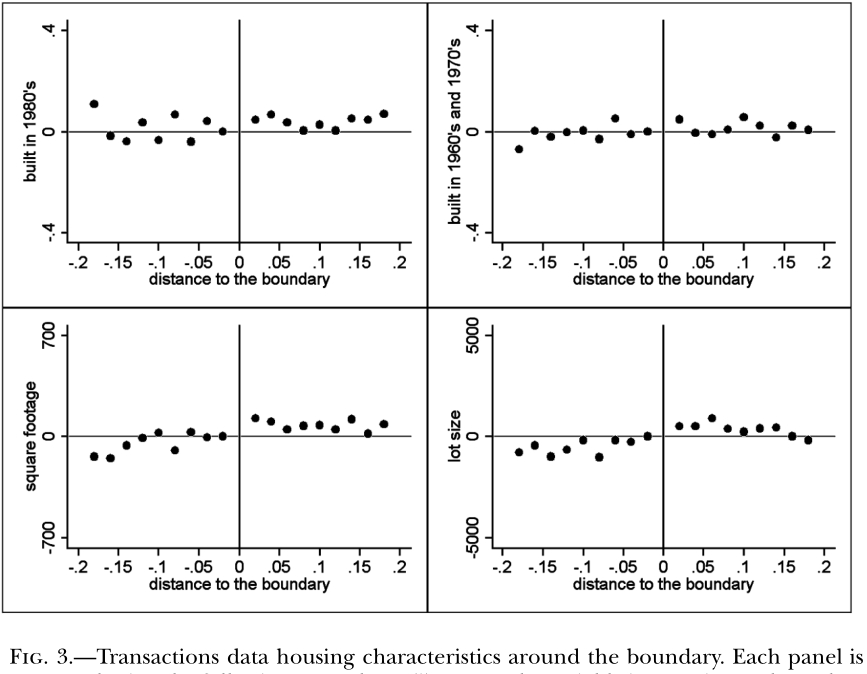
\includegraphics[height = 8cm]{ImpactEvaluation/figure/Bayer_Fig3.jpg}\\
\end{frame}
\begin{frame}{}
\citet{BayerFerreiraMcMillan2007}: 居住者の特徴は境界内外で相違\\
\hfil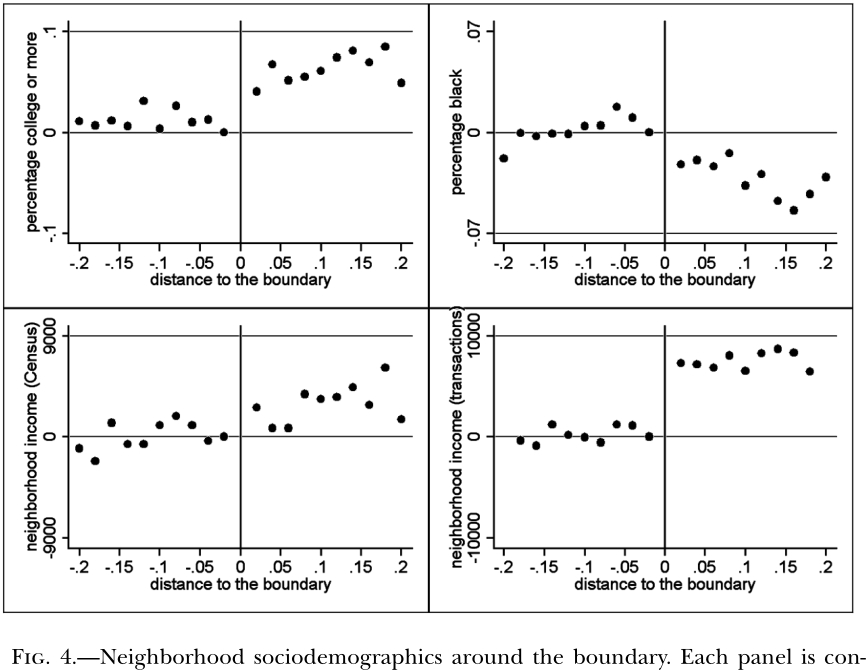
\includegraphics[height = 8cm]{ImpactEvaluation/figure/Bayer_Fig4.jpg}\\
\end{frame}
\begin{frame}{}
\vspace*{-0cm}

\onslide<1->{境界を挟んだ家計同士の比較で親の学歴、所得、人種を共変数に加えて統御、家の使用者費用/月に与える差の効果を推計\\~\\}
\mpage{12cm}{\onslide<2->{
\vspace*{-.5cm}
\mpagethree{7cm}{\hfil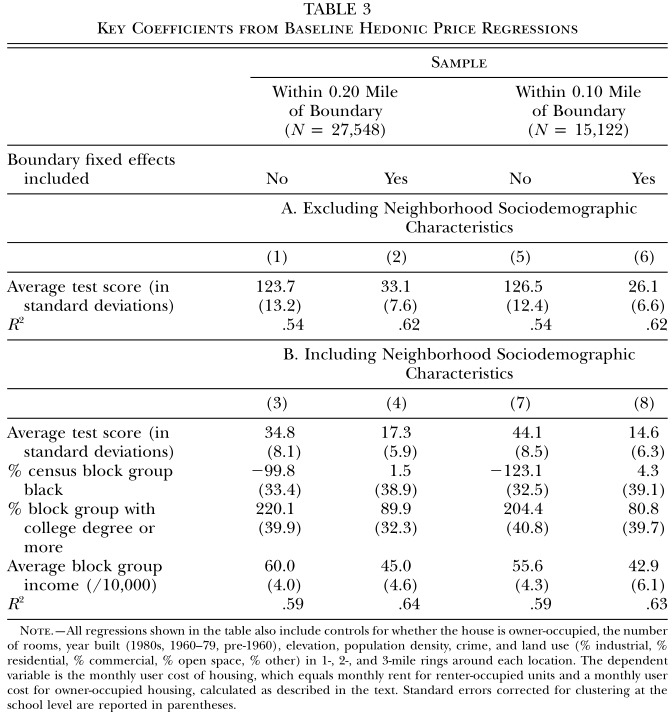
\includegraphics[height = 7cm]{ImpactEvaluation/figure/Bayer_Table3.jpg}\\

\vspace*{-4.9cm}
\mpage{8cm}{
\hspace{3.7cm}\Rect{.5}{.4}{red}\\

\vspace{.45cm}
\hspace{3.7cm}\Rect{.5}{1.73}{red}
}}{c}} \mpagethree{4cm}{
\onslide<3->{各境界線の平均値(boundary fixed effects)を差し引くと試験点数の効果が1/4に減少[A(2)]\\~\\}
\onslide<4->{観察可能な境界線地域の特徴を共変数に加えるとさらに1/2に減少[B(4)]\\~\\}
\onslide<5->{学歴や所得などを統御すると、黒人居住者比率の影響はほぼゼロ[B(4)]}
}{c}
}
\end{frame}

\begin{frame}{}
\citet{Bohlken2018}: インドで与党議員得票率と予算配分\\
\hfil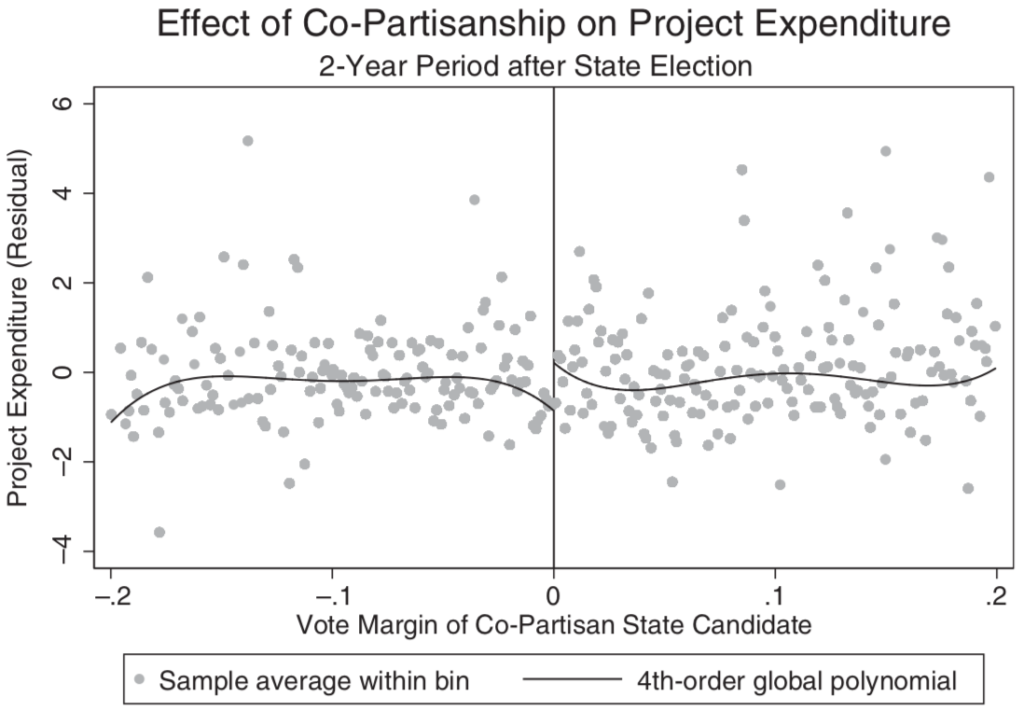
\includegraphics[height = 8cm]{ImpactEvaluation/figure/RDD_BadIndiaCoPartisanship.png}\\
線は4次関数$y=a_{0}+a_{1}x+a_{2}x^{2}+a_{3}x^{3}+a_{4}x^{4}+e$を回帰させた線
\end{frame}

\begin{frame}{}
統計学者\href{https://statmodeling.stat.columbia.edu/author/andrew/}{Andrew Gelman (コロンビア大学、ブログ魔)}:

\begin{quotation}
A global fourth-degree polynomial, huh? This is almost a parody of how to make spurious discoveries. (4次関数? 見せかけの発見のパロディ[つまり、意図的な冗談]みたいだ。)\\~\\

\pause
Those of us who develop advanced statistical methods have to be aware that, once a method is out there, it can be used ``off-label'' by anybody, and lots of those uses will be mistaken in some way or another. No, my problem is the false sense of certainty that appears to be engendered by the use of high-tech statistics. (推計方法が広まると「目的外利用」をする人が必ず出る。にもかかわらず、ハイテク統計学を利用したから推計結果は正しい、と誤った確信を深めていそうなのが問題だ。)
\end{quotation}
\vspace{2ex}
\pause
現在は曲線を伴う関数で回帰することは厳禁とされ、分断近傍で直線を使うことが多い\\
\hfill\beamergotobutton{RDD推計の図解(別ファイル)}
\end{frame}

\begin{frame}{}
\citet{Magaloni2019}: メキシコのオアハカ州で民選か世襲の伝統的指導者による地方自治が混在したときの比較(RDD)\\
\pause
\hfil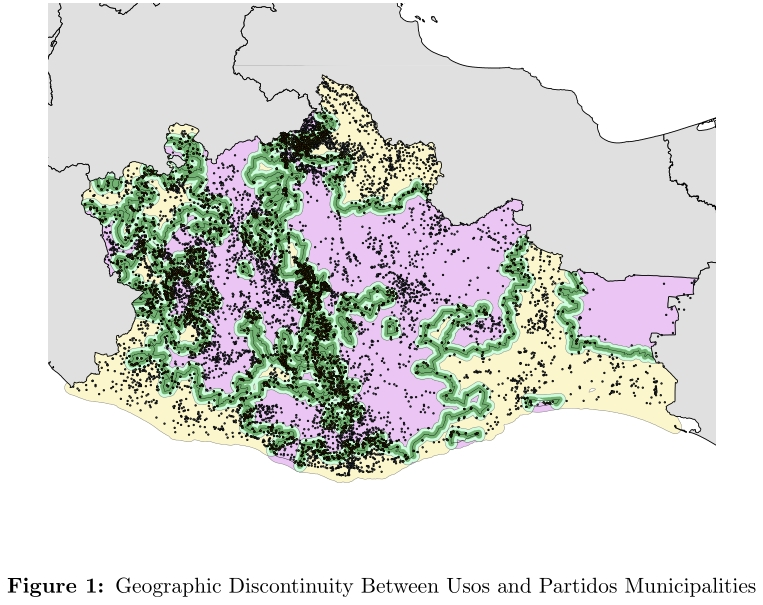
\includegraphics[width = 8cm]{ImpactEvaluation/figure/Magaloni_MexicoUsosFig1.jpg}
\end{frame}

\begin{frame}{}
上水道未整備率、民選首長vs.伝統的指導者\\
\hfil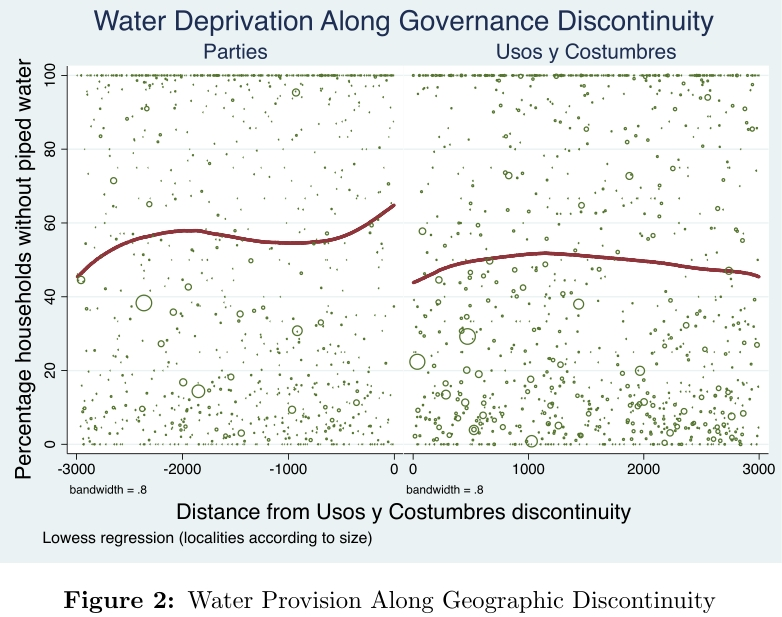
\includegraphics[height = 7cm]{ImpactEvaluation/figure/Magaloni_MexicoUsosFig2.jpg}
\end{frame}

\begin{frame}{}
下水道未整備率、民選首長vs.伝統的指導者\\
\hfil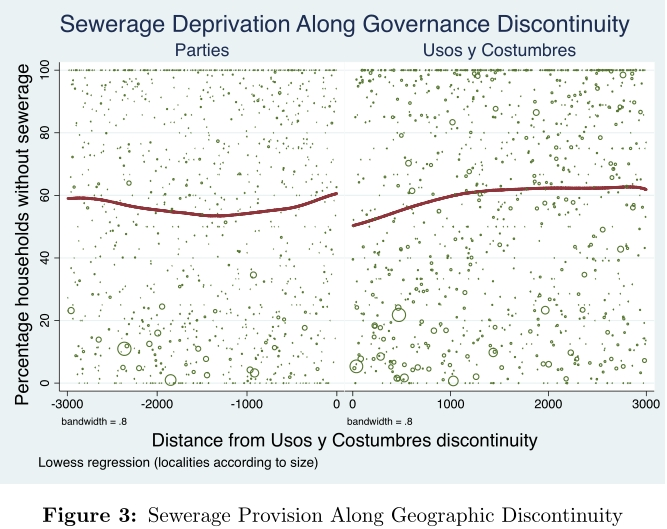
\includegraphics[height = 5cm]{ImpactEvaluation/figure/Magaloni_MexicoUsosFig3.jpg}\\
\pause
何が何だか分からない図\\~\\
\pause
「境界からの距離」だけでは多様な地域同士を比較、政策効果か異質なグループ比較によるノイズか分からない\\~\\
\pause
境界のどの部分か限定する必要: 地形、水源、人口規模、上水道行政単位などが違うと工事の難易度(ノイズ)が入り込む
\end{frame}

\begin{frame}{}
オアハカ(メキシコ)の地図との比較\\~\\
\hfil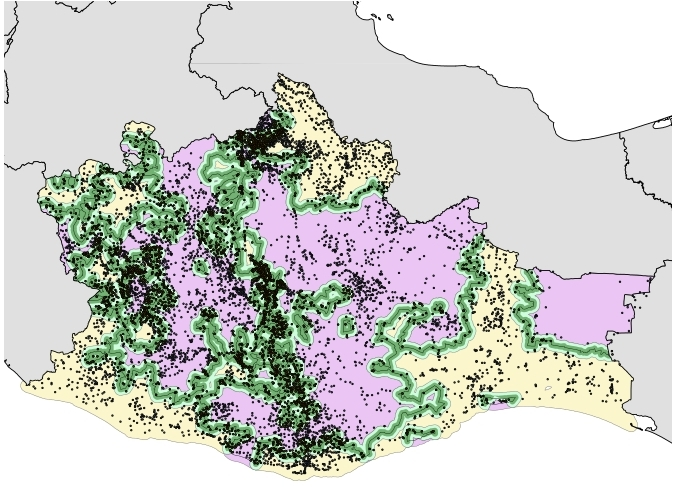
\includegraphics[width = 4cm]{ImpactEvaluation/figure/Magaloni_MexicoUsosFig1NoCaption.jpg}
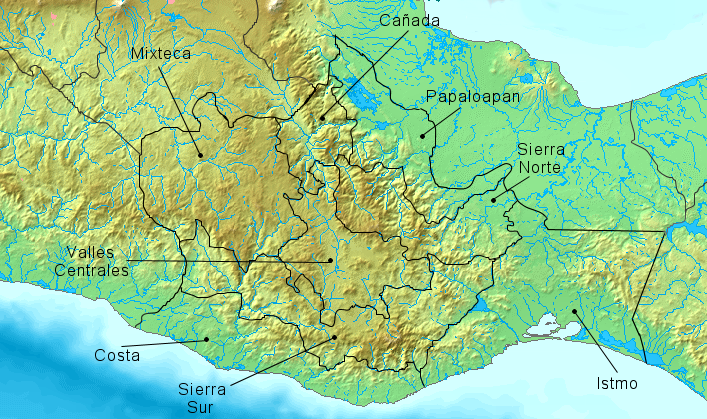
\includegraphics[width = 5cm]{ImpactEvaluation/figure/Oaxaca_fisico_regiones.png}\\
{\footnotesize 出所: 左\citet[][Figure 1]{Magaloni2019}, 右\href{https://commons.wikimedia.org/wiki/Image:Topographic30deg_N0W90.png}{Mario Fuente Cid} 
\includegraphics[height = .3cm]{ImpactEvaluation/figure/CCBy-SA.jpg}}\\~\\
\pause
境界(緑の帯):
\begin{dinglist}{43}
\vspace{1.0ex}\setlength{\itemsep}{1.0ex}\setlength{\baselineskip}{12pt}
\pause
\item	沿岸部平地や河川湖沼の有無を含んで多様
\pause
\item	地形による境界(河川湖沼、山脈)と一致している部分も多くある
\pause
\item	自治形態ではなく地形が原因で上水道普及率がジャンプしている可能性あり\\~\\
\end{dinglist}
\pause
use your common senseとGelmanに怒られそう...
\end{frame}


\begin{frame}[t]{Go To Eatの効果?}
\begin{columns}[T]
\column{.5\paperwidth}
日経新聞2020年11月23日(月)朝刊\\
\begin{tikzpicture}[inner sep=0pt, remember picture]
\node at (0, 0) {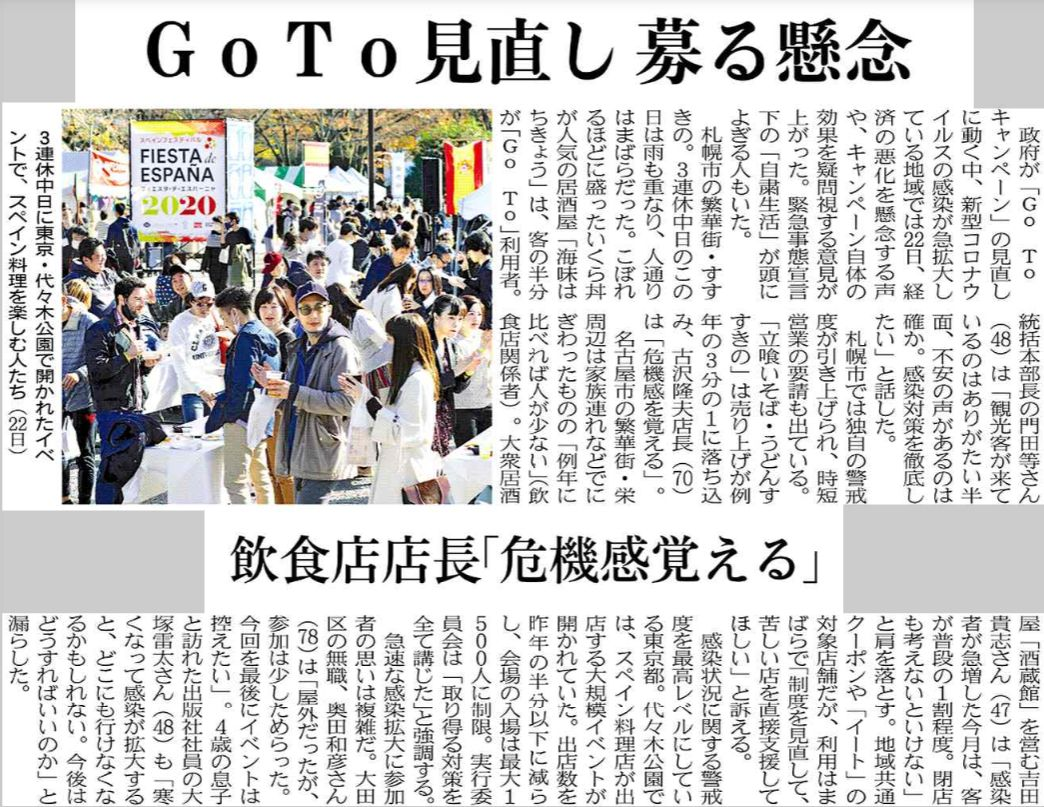
\includegraphics[clip, width = .5\paperwidth]{ImpactEvaluation/figure/Nikkei_GoToMinaoshiKenen2020Nov23.jpg}};
\onslide<2->{\node (a) [draw, rectangle, thick, rounded corners, minimum height = 1.75cm, minimum width = .5cm, red] at (.05cm, 1.5cm){};
}
\end{tikzpicture}
\column{.4\paperwidth}
\onslide<2->{
\begin{tikzpicture}[inner sep=0pt, remember picture]
\node (b) at (0, 0) {「客の半分が『Go To』利用者」};
\end{tikzpicture}\\~\\
}
\onslide<3->{
「『Go To』利用者」=Go To Eatの効果でしょうか?\\~\\
}
\onslide<4->{
GoToなしでも、もともと行くつもりだったかも。\\~\\
}
\onslide<5->{
Go To Eatの効果を測定できる研究デザインとは?\\	
}
\onslide<6->{
ランダム化比較試験、SCM(synthetic control method)など\\~\\
}
\onslide<7->{
どんな方法かは後で説明します
}
\end{columns}
\onslide<2->{
\begin{tikzpicture}[remember picture, overlay]
\draw[red, very thick, ->] (b.west) to [out=180, in=0] (a.east);
\end{tikzpicture}
}
\end{frame}



\begin{frame}[t]{GoToトラベルの効果?}
2020年12月14日(月)GoToトラベル全国一斉一時停止\\~\\
\begin{columns}[T]
\onslide<1->{
\column{.5\paperwidth}
{\footnotesize FNNプライムニュース2020年11月25日(水)}\\
\hfil
\includegraphics[clip, width = .5\paperwidth]{ImpactEvaluation/figure/Suga_NoEvidenceCropped.jpg}
}
\column{.4\paperwidth}
\onslide<2->{
エビデンス=科学的な方法で明らかになった事象
}
\onslide<3->{
\begin{dinglist}{45}
\vspace{1.0ex}\setlength{\itemsep}{1.0ex}\setlength{\baselineskip}{12pt}
\item	科学的な方法: 反証可能な命題が成立するか検定する方法\\~\\
\end{dinglist}
}

\onslide<4->{
エビデンスがないのは事実
}
\begin{dinglist}{43}
\vspace{1.0ex}\setlength{\itemsep}{1.0ex}\setlength{\baselineskip}{12pt}
\onslide<5->{
\item	政府は効果検証用にデータを収集していないため
}
\onslide<6->{
\item	検証するつもりなし、と言っているに等しい\\~\\
}
\end{dinglist}
\end{columns}

\onslide<7->{
利用可能なデータを前提にすると、どのような効果検証が可能か?
}
\end{frame}

\begin{frame}[t]{GoToトラベルの効果?}
2020年12月14日(月)GoToトラベル全国一斉一時停止\\~\\
\pause
{\footnotesize\url{http://www.kantei.go.jp/jp/99_suga/statement/2022/1214kaiken02.html}\\}
記者「GoToトラベルに感染拡大のエビデンスがないとの認識はあったか?」\\
(NHKサイトでは「GoToトラベルに感染拡大のエビデンスはないという認識は変わったのか」)\\~\\

\pause
管首相
\mpage{\textwidth}{\footnotesize 「そこは、\textcolor{red}{医師会の会長が申し上げている}のではないでしょうか。それと、当時は\textcolor{red}{移動によっては、感染を拡大しないということ、ここも提言もあります}。そこについては変わりません。ただ、今回そうしたことの専門家の委員の先生方からそういう指摘をいただきましたので、この3000人、\textcolor{red}{現実的に患者の方が出ていますから、}年末年始、集中的に対応できる、そういうチャンスだと、そういう思いの中で私は判断しました。」\setlength{\baselineskip}{9pt}}\\~\\

\pause
エビデンスはなく(と会長が言っている)、移動は感染を広げないと(誰から?)聞いていたが、感染者数が増えたから停止、という主張
\end{frame}

\begin{frame}[t]{GoToトラベルの効果?}
2020年12月14日(月)GoToトラベル全国一斉一時停止\\~\\
\pause
2020年11月18日(水)日本医師会会長中川氏\\
\mpage{\textwidth}{\footnotesize 「GoToトラベル自体から感染者が急増したというエビデンス(根拠)はなかなかはっきりしないが、きっかけになったことは間違いないと私は思っている。感染者が増えたタイミングを考えると関与は十分しているだろう」\setlength{\baselineskip}{9pt}}
\begin{dinglist}{43}
\vspace{1.0ex}\setlength{\itemsep}{1.0ex}\setlength{\baselineskip}{12pt}
\pause
\item	原因ではないがきっかけ、というのは意味不明\\~\\
\end{dinglist}

\pause
2020年12月16日(水)衆院内閣閉院中審査: {\scriptsize 新型コロナウィルス感染症対策分科会}尾身会長\\
\mpage{\textwidth}{\footnotesize 「50歳以下の人が移動して二次感染を起こしていることがはっきりしきたので、人の動きを止めることが重要で、その一環のなかでGoToトラベルもある。」「本質は意図せず重症化が出るので、そのような文脈のなかでGoToトラベルも考えるべきと再三申し上げている。」\setlength{\baselineskip}{9pt}}
\begin{dinglist}{43}
\vspace{1.0ex}\setlength{\itemsep}{1.0ex}\setlength{\baselineskip}{12pt}
\item	「移動は感染を拡大させない」という提言はない。
\item	50歳以下が感染伝播の高リスク・グループと判明、この移動を制限すべき、という提言。GoToトラベルによる感染拡大のエビデンスではないが、論理的帰結によって制限を結論。
\end{dinglist}
\end{frame}

\begin{frame}[t]{GoToトラベルの効果?}
2020年12月14日(月)GoToトラベル全国一斉一時停止\\~\\
因果関係を検定できるデータを集めることが大事\\
\pause
ただし、政策担当者の協力なしには効果推計に限界がある\\~\\
\pause
\begin{dinglist}{43}
\vspace{1.0ex}\setlength{\itemsep}{1.0ex}\setlength{\baselineskip}{12pt}
\item	GoToトラベル利用者にはCOCOA導入と登録を条件付けてもよかったかもしれない
\item	GoToトラベル利用中に感染や濃厚接触をするリスクを計算できる
\item	GoToトラベル期間ごとに、たとえば、11月第1週に予算を幾ら支出したら、利用者がどれだけいて、こうしたリスクがこれだけ高まった、と計算できる
	\begin{dinglist}{45}
	\vspace{1.0ex}\setlength{\itemsep}{1.0ex}\setlength{\baselineskip}{12pt}
	\item	それでも、補助金に関係なく行く人たちもいるので、GoToTravelの効果だけではない、過大推計
	\item	補助金に関係なく行く人たちの分を差し引く必要あり
	\end{dinglist}
\end{dinglist}
\end{frame}

\begin{frame}[t]{GoToトラベルの効果?}
効果推計の例
\begin{itemize}
\vspace{1.0ex}\setlength{\itemsep}{2.0ex}\setlength{\baselineskip}{12pt}
\item	旅客人数: 前年度同月値との比較
\item	旅行支出: 推計した需要関数が正しいと前提に補助金の効果を試算
\item	(有症率比較: GoToトラベル利用者 vs. 非利用者)
\item	ビッグ・データによる人の移動: \\
\hspace{1em}GoToトラベル開始前後の変化-昨年同時期の変化
\item	グレンジャー因果性: 航空旅行客と感染者数の関係
\item	合成統御法: GTT東京追加と東京圏感染者数の関係
\end{itemize}
\end{frame}

\begin{frame}[t]{GoToトラベルの効果?}
よくある比較\\~\\
\pause
GoToトラベル実施月の旅客人数を前年度同月値と比較して「x\%多かった」と示す\\~\\
\pause
昨年度と比較=GoToトラベルなしだと昨年と同じという(暗黙の?)仮定をしている
\begin{description}
\vspace{1.0ex}\setlength{\itemsep}{1.0ex}\setlength{\baselineskip}{12pt}
\pause
\item[被説明変数]	旅客人数
\pause
\item[データ]	国土交通省データ
\pause
\item[識別仮定identification assumption]	「GoToトラベルがなければ、今年も昨年と同じ人の移動だった」
	\begin{dinglist}{43}
	\vspace{1.0ex}\setlength{\itemsep}{1.0ex}\setlength{\baselineskip}{12pt}
\pause
	\item	このデザインでの効果推計値の信頼性=この識別仮定の現実妥当性
	\end{dinglist}
\end{description}
\end{frame}

\begin{frame}[t]{GoToトラベルの効果?}
\begin{description}
\vspace{1.0ex}\setlength{\itemsep}{1.0ex}\setlength{\baselineskip}{12pt}
\item[課題] 
	\begin{enumerate}
	\vspace{1.0ex}\setlength{\itemsep}{1.0ex}\setlength{\baselineskip}{12pt}
\pause
	\item	GoToトラベルなしのとき、移動人数が当該年と前年で同じと期待する理由はない。おそらく、GoToトラベルなしだとGoToトラベル実施年は景気後退でその前年より少なかったはず。(分母=なしのときの水準が過大なので)水準との比による評価は過小評価になる。
\pause
	\item	2020年(GoToトラベル実施時)に入国制限されたインバウンド客を除外して2019年のデータを作成できるか? 
	\end{enumerate}
\end{description}

\pause
\vspace{2ex}
誰にでもできる分析なので、何と比較すべきかを考えずにやっている人が多いはず\\~\\
\pause
「今年はコロナウィルス流行によって大きく減っているという事情はありますが」などという数字以外の補正をして説明するはず\\~\\
\pause
効果があったのかはっきりしないし、聞き手の主観が入り込む
\end{frame}


\begin{frame}[t, label=GTTElasticity]{GoToトラベルの効果?}
需要関数を使った試算\\~\\
野村総研木内氏「東京除外で減少するGo Toトラベルの消費押し上げ効果は1.5兆円程度か」{\scriptsize \url{https://www.nri.com/jp/knowledge/blog/lst/2020/fis/kiuchi/0717}}\\

\begin{columns}[T]
\column{.7\paperwidth}
\onslide<2->{
\mpage{.7\paperwidth}{\footnotesize 「 内閣府の分析によると、\textcolor{red}{サービス消費の価格弾性値は-0.8}である。これは、価格が1%低下すると実質サービス消費は0.8\%増加する傾向にある、ということを意味している。」「ところで、『Go Toトラベル』では旅行費用が半分になる、つまり\textcolor{red}{50\%の値下げ}が実施されるに等しくなるため(上限を超える支出部分は考慮しない)、それは支援の対象となる旅行関連消費を\textcolor{red}{40\%増加}させる計算だ(支援部分も含む)。」\setlength{\baselineskip}{9pt}}
}
\column{.25\paperwidth}
\onslide<3->{
\begin{dinglist}{43}
\vspace{0.0ex}\setlength{\itemsep}{1.0ex}\setlength{\baselineskip}{12pt}
\item	50\%$\times$.8=40\%
\end{dinglist}
\hfill\hyperlink{WhyUseElasticity}{\beamergotobutton{需要の価格弾力性}}
}
\end{columns}

\vspace{2ex}
\begin{columns}[T]
\column{.7\paperwidth}
\onslide<4->{
\mpage{.7\paperwidth}{\footnotesize 「観光庁によれば、日本人の国内旅行の関連消費額は、2017年に\textcolor{red}{21.5兆円}と、個人消費全体の7.1%を占めている。これが\textcolor{red}{40\%}増加すれば、1年間で消費を\textcolor{red}{8.7兆円}増加させる。」\setlength{\baselineskip}{9pt}}
}
\column{.25\paperwidth}
\onslide<5->{
\begin{dinglist}{43}
\vspace{0.0ex}\setlength{\itemsep}{1.0ex}\setlength{\baselineskip}{12pt}
\item	21.5兆円$\times$.4 =8.60兆円
\end{dinglist}
}
\end{columns}

\vspace{2ex}
\begin{columns}[T]
\column{.7\paperwidth}
\onslide<6->{
\mpage{.7\paperwidth}{\scriptsize 「内閣府の県民経済計算(平成28年度)によると、東京都の都民所得は全国の\textcolor{red}{17.8\%}である。この比率分...(中略)...(感染への警戒から、東京着の旅行は現在かなり少ないとみられるため、ここでは東京発の旅行のみ考慮する)、今回の東京の除外によって、「Go Toトラベル」の消費押し上げ効果は1年間で\textcolor{red}{1.54兆円減少}し、1年間のGDP成長率の押し上げ効果を0.28\%減らす計算となる。」\setlength{\baselineskip}{8pt}}
}
\column{.25\paperwidth}
\begin{dinglist}{43}
\vspace{0.0ex}\setlength{\itemsep}{1.0ex}\setlength{\baselineskip}{12pt}
\onslide<7->{
\item	8.6兆円$\times$.178 =1.53兆円
}
\end{dinglist}
\end{columns}
\end{frame}

\begin{frame}[t, label=GTTElasticity2]{GoToトラベルの効果?}
需要関数を使った試算\\~\\
野村総研木内氏「東京除外で減少するGo Toトラベルの消費押し上げ効果は1.5兆円程度か」{\scriptsize \url{https://www.nri.com/jp/knowledge/blog/lst/2020/fis/kiuchi/0717}}\\~\\

\pause
需要関数を使って影響を考えるのはよいことだが、2020年以前のデータを使って推計されたCOVID以前の需要関数をCOVID下の2020年の需要関数として利用\\~\\
\pause
2020年は旅行需要が価格と無関係に萎縮しているはず\\~\\
\pause
萎縮した2020年需要関数の価格弾力性はCOVID以前の価格弾力性と同じ保証はない\\~\\
\pause
情報が無いながらもやってみる、というスタンスならば、その留意を明記すべき
\end{frame}

\begin{frame}[t, label=GTTElasticity3]{GoToトラベルの効果?}
需要関数を使った試算\\~\\
野村総研木内氏「GOTOトラベル見直しとその経済効果の試算」{\scriptsize \url{https://www.nri.com/jp/knowledge/blog/lst/2020/fis/kiuchi/1124}}\\
\begin{columns}[T]
\column{.7\paperwidth}
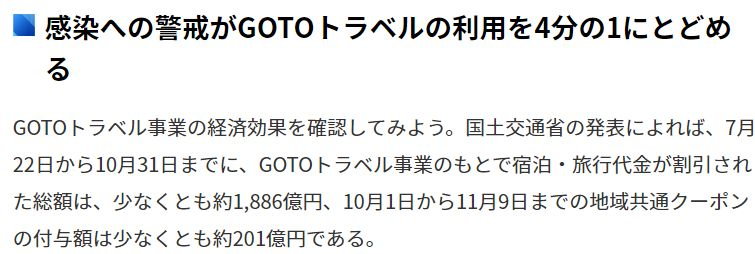
\includegraphics[clip, height = 2cm]{ImpactEvaluation/figure/KiuchiGoTo.jpg}
\column{.25\paperwidth}
\begin{dinglist}{43}
\vspace{1.0ex}\setlength{\itemsep}{1.0ex}\setlength{\baselineskip}{12pt}
\item	GoToトラベル利用総額1886億円
\end{dinglist}
\end{columns}

\vspace{2ex}
\begin{columns}[T]
\column{.7\paperwidth}
\onslide<2->{
\mpage{.7\paperwidth}{\footnotesize 「宿泊・旅行代金の\textcolor{red}{35\%}に相当する割引額から、その間のGOTOトラベルを利用した全体の旅行支出額を計算すると、\textcolor{red}{5,389億円}となる。必ずしも正確ではないが、(中略)さらに東京が除外されていなかった場合(中略)、推定で6,150億円、月間平均で1,809億円、年換算で2兆1,708億円となる。」\setlength{\baselineskip}{9pt}}
}
\column{.25\paperwidth}
\onslide<3->{
\begin{dinglist}{43}
\vspace{1.0ex}\setlength{\itemsep}{1.0ex}\setlength{\baselineskip}{12pt}
\item	1886億円/.35 =5389億円
\end{dinglist}
}
\end{columns}
\begin{dinglist}{43}
\vspace{1.0ex}\setlength{\itemsep}{1.0ex}\setlength{\baselineskip}{12pt}
\onslide<4->{
\item	「東京が除外されていなかった場合、推定で6150億円」をどうやって計算したのか不明。効果推計で最も大事な部分を解説していないのはまともではない。
}
\end{dinglist}
\end{frame}

\begin{frame}[t, label=GTTElasticity4]{GoToトラベルの効果?}
需要関数を使った試算\\~\\
野村総研木内氏「GOTOトラベル見直しとその経済効果の試算」{\scriptsize \url{https://www.nri.com/jp/knowledge/blog/lst/2020/fis/kiuchi/1124}}\\~\\

\mpage{.9\paperwidth}{\footnotesize 「ところで、GOTOトラベル事業は、国内旅行需要を1年間で8.7兆円増加させると試算される(コラム「東京除外で減少するGo Toトラベルの消費押し上げ効果は1.5兆円程度か」、2020年7月17日)。この試算値に対して、実績値は4分1にとどまっている計算だ。その分、感染への警戒が、GOTOトラベルを利用した旅行需要を減少させている、と考えることができる。」\setlength{\baselineskip}{9pt}}\\~\\

\begin{columns}[T]
\column{.475\paperwidth}
\onslide<2->{
「東京除外でない場合のGoToトラベルによる増加試算額8.7兆円」は絶対値で1よりも小さい点弾力性を使っている
\begin{dinglist}{43}
\vspace{1.0ex}\setlength{\itemsep}{1.0ex}\setlength{\baselineskip}{12pt}
\item	需要曲線の左側=直線により近い\\
\onslide<3->{
$\Rightarrow$過大推計になりやすい\\~\\
}
\end{dinglist}
}
\column{.475\paperwidth}
\onslide<4->{
「除外されていなかった場合の試算額」-実績額=感染への警戒による減少額、は乱暴な議論。試算額が過大だっただけかも。
}
\end{columns}
\end{frame}

\begin{frame}[t]{GoToトラベルの効果?}
需要関数を使った試算\\~\\
\pause
用いたデータと推計方法が適切ならば、理想的な効果試算方法
\begin{dinglist}{43}\footnotesize
\vspace{1.0ex}\setlength{\itemsep}{1.0ex}\setlength{\baselineskip}{12pt}
\pause
\item	需要関数とは消費者の効用最大化から求められるので、経済理論の裏付けがある
\pause
\item	原典は内閣府「日本経済2018-2019」白書第3章付注2-3、推計方法(QUAIDS消費関数をFGNLS)、データは総務省「家計調査」
\pause
\item	データは理想的、推計方法も標準的
\end{dinglist}

\pause
\vspace{2ex}
しかし、COVID以前の推計結果を使って良いわけがない\\~\\
\pause
さらに、価格弾性値の扱いが不適切
\begin{dinglist}{43}\footnotesize
\vspace{1.0ex}\setlength{\itemsep}{1.0ex}\setlength{\baselineskip}{12pt}
\pause
\item	内閣府推計値は点弾力性point elasticityで非弾力的、過大推計になりやすい
\pause
\item	乗じる50\%は大きな価格変化$\Delta p$なので、推計された需要変化は一層過大
\end{dinglist}
\pause
\vspace{2ex}
経済理論を使って厳密そうな印象だが、印象で判断してはいけない
\end{frame}

\begin{frame}[t]{GoToトラベルの効果?}
\begin{columns}[T]
\column{.475\paperwidth}
\includegraphics[clip, height = 6cm]{ImpactEvaluation/figure/TokyoShinbun_GoToCovid.jpg}
\column{.475\paperwidth}
「GoToトラベル利用者感染リスク高い」東京大学など研究チーム\\
2020年12月8日(火)\\
論文: \citet{Miyawaki2020}
\end{columns}
\end{frame}

\begin{frame}[t]{GoToトラベルの効果?}
「GoToトラベル利用者感染リスク高い」東京大学など研究チーム\\~\\
研究デザイン
\begin{itemize}
\vspace{1.0ex}\setlength{\itemsep}{1.0ex}\setlength{\baselineskip}{12pt}
\item	インターネット調査(楽天インサイト社実施)、22万4389人中2万8000人回答、2万5482人有効回答
\item	症状有無、GoToトラベル利用有無、社会経済変数、既往症\\~\\
\end{itemize}

\pause
GoToトラベル利用者は非利用者よりも有症率が2倍\\~\\
\pause
解釈: 以下の可能性がある
\begin{enumerate}
\vspace{1.0ex}\setlength{\itemsep}{1.0ex}\setlength{\baselineskip}{12pt}
\pause
\item	GoToトラベルで罹患
\pause
\item	有症率(=罹患確率)の高い人がGoToトラベル利用\\~\\
\end{enumerate}
\pause
結論: 「リスクの低い人に経済活動の誘因を与え、高い人は自宅待機を促すべき」
\end{frame}

\begin{frame}[t]{GoToトラベルの効果?}
「GoToトラベル利用者感染リスク高い」東京大学など研究チーム\\~\\
閣僚の反応{\scriptsize\url{https://news.tbs.co.jp/newseye/tbs_newseye4146048.htm?1607587275057}}\\~\\

\begin{description}
\vspace{1.0ex}\setlength{\itemsep}{1.0ex}\setlength{\baselineskip}{12pt}
\item[田村憲久厚労相]	「ちょっとエビデンスといえるものなのかどうなのか、ちょっと査読も終わっていないという話ですし。評価のしようがないというのが、正直なところでありますので」
\item[赤羽一嘉国交相]	「この論文についても、ちょっと正式に査読前という話もありましたし。現時点では全くコメントする段階でないと思っている」
\item[加藤勝信官房長官]	「著者自らもですね、研究方法の限界として、GoToトラベルの利用が直接的に新型コロナ症状の増加につながったという因果関係は断定できないこと」
\end{description}

\end{frame}

\begin{frame}[t]{GoToトラベルの効果?}
「GoToトラベル利用者感染リスク高い」東京大学など研究チーム\\~\\
示した解釈が面白いし、明確な政策提言になっている\\~\\
結果の提示も慎重「因果関係を示している訳ではない」\\~\\
\pause
しかし...\pause この研究には方法論として弱点があると思います\\~\\
\pause
何でしょうか?\\~\\

\pause
空いたスペースで政治家の反応への疑問
\begin{dinglist}{43}
\vspace{1.0ex}\setlength{\itemsep}{1.0ex}\setlength{\baselineskip}{12pt}
\pause
\item	査読通ったら意見、対応するのか?
\pause
\item	実験は存在しないので因果関係は示せない。では、どんな事実があれば対応するのか?エビデンスなんて出てこないことを知っていながらの、何もしない言い訳では?
\pause
\item	単にケチ付けているだけでは?
\end{dinglist}
\end{frame}

\begin{frame}[t]{GoToトラベルの効果?}
「GoToトラベル利用者感染リスク高い」東京大学など研究チーム\\~\\
示したこと: 有症率(A)とGoToトラベル利用(B)の正の相関\\~\\
\pause
検討していない可能性: みせかけの相関\\~\\
\pause
その他の現象(C)が(A)と(B)を同時に動かしているのでは?\\~\\
\pause
Cの例: 外出量\\~\\
\pause
外出好きな人は罹患確率[$\propto$有症率(A)]が高い\\~\\
\pause
外出好きな人は旅行をよくする(行くのだったら割引を使う)\\~\\
\pause
外出好きな人は罹患しやすく、旅行も頻繁にする、というだけでは?\\~\\
\pause
もしもそうだったら、結論は常識の範囲内
\end{frame}

\begin{frame}[t]{GoToトラベルの効果?}
「GoToトラベル利用者感染リスク高い」東京大学など研究チーム\\~\\
政策提言が実施困難: どうやって個人の感染させるリスクを判断するのか?
\begin{dinglist}{43}
\vspace{1.0ex}\setlength{\itemsep}{1.0ex}\setlength{\baselineskip}{12pt}
\pause
\item	年齢: 年齢差別になりかねず、違憲の可能性あり
\end{dinglist}
\pause
\vspace{2ex}
もしも可能だったら...ランダムにGoToトラベル資格を配布する実験をする\\~\\
\pause
有資格者と無資格者の有症率の違いを検定する: 明確な因果関係\\~\\
\pause
でも、有資格者と周辺者が危険に曝される可能性があるので、研究倫理審査委員会が却下するかも\\~\\
\pause
GoToトラベル=研究倫理審査委員会が却下しかねない政策
\end{frame}


\begin{frame}[t]{GoToトラベルの効果?}
「GoToトラベル利用者感染リスク高い」東京大学など研究チーム\\~\\
普段の外出頻度を尋ねていれば、外出頻度を制御して比較%。外出頻度に影響されずにGoToトラベル利用の有無による有症確率$\Pr(\mbox{有症})$の比較ができる
\pause
\[
\Delta \Pr(\mbox{有症}|\mbox{外出多})=\Pr[\mbox{有症}|\mbox{外出多, \textcolor{azure}{GoTo利用}}]-\Pr[\mbox{有症}|\mbox{外出多, \textcolor{azure}{GoTo非利用}}].
\]
\pause
外出頻度ごとに帰無仮説を検定
\[
\begin{aligned}
H_{01}&: \Delta \Pr(\mbox{有症}|\mbox{外出少})=0\\
H_{02}&: \Delta \Pr(\mbox{有症}|\mbox{外出多})=0
\end{aligned}
\]
仮に、それぞれの帰無仮説において$p$ valueが小さい\\
 $\Rightarrow$ 外出頻度同程度の人でGoToトラベルと有症率に正の相関関係\\
 $\Rightarrow$ GoToトラベルが有症率を高める因果関係と矛盾しない\\~\\
\pause
残念ながら、外出頻度は尋ねていない模様。\pause
デザイン段階でもう少し考えるべきだったかも?
\end{frame}


\begin{frame}[t]{GoToトラベルの効果?}
ビッグ・データによる人の移動
\begin{description}
\vspace{1.0ex}\setlength{\itemsep}{1.0ex}\setlength{\baselineskip}{12pt}
\item[被説明変数]	移動人数
\item[データ]	スマートフォン・データ
\item[効果]	$\underbrace{\mbox{GoToトラベル開始前後の変化}}_{\mbox{2020年の8月前後変化}}-\underbrace{\mbox{昨年同時期の変化}}_{\mbox{2019年の8月前後変化}}$
\item[推計量]	二重差分推計量double difference (difference-in-differences, DID) estimator: 今年の変化と比較対象の変化の差(差分と差分の差=二重差分)を政策の効果と見なす。
\end{description}
\end{frame}

\begin{frame}[t]{GoToトラベルの効果?}
ビッグ・データによる人の移動
\begin{description}
\vspace{1.0ex}\setlength{\itemsep}{1.0ex}\setlength{\baselineskip}{12pt}
\item[長所]	被説明変数(出典ビッグ・データ)が正確、高頻度、即時。昨年同時期比較で季節性を制御。
\item[短所]	信頼性の低さ。感染者数ではなく移動人数という間接指標を使っていること。
\item[識別仮定identification assumption]	「GoToトラベルがなければ、今年も昨年と同じ人の移動人数変化だった」
	\begin{dinglist}{43}
	\vspace{1.0ex}\setlength{\itemsep}{1.0ex}\setlength{\baselineskip}{12pt}
	\item	このデザインでの効果推計値の信頼性=この識別仮定の現実妥当性
	\end{dinglist}
\item[課題] 
	\begin{enumerate}
	\vspace{1.0ex}\setlength{\itemsep}{1.0ex}\setlength{\baselineskip}{12pt}
	\item	GoToトラベルなしのとき、移動人数の変化(傾き)が今年と昨年で同じと期待する理由はない。おそらく、GoToトラベルなしだと今年は増加幅が去年より小さかったはず。過小評価になる。
	\item	インバウンド客を除外した昨年のデータを作成できるか? インバウンド客を除外することで移動人数の変化が増えるのか減るのか不明。
	\end{enumerate}
\end{description}
\end{frame}

\tikzset{
  shifted path/.style args={from #1 to #2 by #3}{insert path={
    let \p1=($(#1.east)-(#1.center)$),
    \p2=($(#2.east)-(#2.center)$),\p3=($(#1.center)-(#2.center)$),
    \n1={veclen(\x1,\y1)},\n2={veclen(\x2,\y2)},\n3={atan2(\y3,\x3)} in
    (#1.{\n3+180+asin(#3/\n1)}) to (#2.{\n3-asin(#3/\n2)})
}}}

\setbeamercovered{invisible}
\begin{frame}[t]{GoToトラベルの効果?}
グレンジャー因果性Granger causality: $A$ Granger-causes $B$\\~\\
\begin{columns}[T]
\column{.75\paperwidth}
\hfil\begin{tikzpicture}[
every node/.style = {color = blue}
]
\path 
	(3, 3) node [shape = circle, draw, fill = blue!25] (A1) {現在の$A$}
	(3, 0) node [shape = circle, draw, fill = red!25] (B1) {現在の$B$};
\onslide<2-6>{
	\draw [->, >= stealth', red] (A1) -- (B1);
	\draw[->, >= stealth', blue, shifted path=from B1 to A1 by 5pt];
}
\onslide<3->{
	\path 
		($(A1) + (3.5, 0)$) node [shape = circle, draw, fill = blue!50] (A2) {過去の$A$}
		($(B1) + (3.5, 0)$) node [shape = circle, draw, fill = red!50] (B2) {過去の$B$};
}
\onslide<4-6>{
	\draw[->, >= stealth', blue, shifted path=from B1 to A2 by 5pt];
	\draw[->, >= stealth', blue, shifted path=from B1 to B2 by 5pt];
}
\onslide<4->{
	\draw [->, >= stealth', red] (A2) -- (B1);
	\draw [->, >= stealth', red] (B2) -- (B1);
}
\onslide<5->{
	\path 
		($(A1) + (-3.5, 0)$) node [shape = circle, draw, fill = blue!10] (A3) {将来の$A$}
		($(B1) + (-3.5, 0)$) node [shape = circle, draw, fill = red!10] (B3) {将来の$B$};
}
\onslide<6>{
	\draw [->, >= stealth', red] (A3) -- (B1);
	\draw [->, >= stealth', red] (B3) -- (B1);
	\draw[->, >= stealth', blue, shifted path=from B1 to A3 by 5pt];
	\draw[->, >= stealth', blue, shifted path=from B1 to B3 by 5pt];
}
\end{tikzpicture}
\column{.2\paperwidth}
矢印は現在の$B$に関わるもののみ表示(他は無視)\\~\\
\onslide<8>{
過去の$B$を考慮にした上で過去の$A$が現在の$B$と相関があること
}
\end{columns}
\end{frame}


\begin{frame}[t]{GoToトラベルの効果?}
グレンジャー因果性Granger causality: $A$ Granger-causes $B$\\~\\

\begin{columns}[T]
\column{.7\paperwidth}
\hspace{10cm}\tikzmark{right}

\mpage{10cm}{
\begin{dinglist}{43}
\vspace{2.0ex}\setlength{\itemsep}{1.0ex}\setlength{\baselineskip}{12pt}
\onslide<1->{\item	現在の$A$は?\hfill\tikzmark{1st}}
\onslide<2->{\item	将来の$B$を見越して現在の$B$が変化している場合は? 現在の$B$を見越して過去の$B$が変化している場合は? }
\onslide<3->{\item	将来の$B$を見越して現在の$A$が変化している場合は? 現在の$B$を見越して過去の$A$が変化している場合は?\hfill\tikzmark{3rd}}
\onslide<4->{\item	本来のG因果性ならば遡れるだけの過去の$A$との相関を推計するが、どこまで遡るべきかは考慮している現象次第}
\end{dinglist}
}
\column{.25\paperwidth}
\begin{adjustbox}{max size={.25\paperwidth}{.3\paperheight}}
\begin{tikzpicture}[
every node/.style = {color = blue}
]
\path 
(3, 3) node [shape = circle, draw, fill = blue!25] (A1) {���݂�$A$}
(3, 0) node [shape = circle, draw, fill = red!25] (B1) {���݂�$B$};
\path 
	($(A1) + (3.5, 0)$) node [shape = circle, draw, fill = blue!50] (A2) {�ߋ���$A$}
	($(B1) + (3.5, 0)$) node [shape = circle, draw, fill = red!50] (B2) {�ߋ���$B$};
\draw [->, >= stealth', red] (A2) -- (B1);
\draw [->, >= stealth', red] (B2) -- (B1);
\path 
	($(A1) + (-3.5, 0)$) node [shape = circle, draw, fill = blue!10] (A3) {������$A$}
	($(B1) + (-3.5, 0)$) node [shape = circle, draw, fill = red!10] (B3) {������$B$};
\end{tikzpicture}

\end{adjustbox}
\end{columns}


\onslide<5->{
\begin{tikzpicture}[overlay, remember picture]
\node[anchor=base] (a) at (pic cs:1st) {\vphantom{h}}; % push the mark to the top of the line (ie including ascenders)
\node[anchor=base] (b) at (pic cs:3rd) {\vphantom{g}}; % push the mark to the bottom of the line (ie including descenders)
\draw [decoration={brace, amplitude=0.5em}, decorate, ultra thick, azure]
  (a.north -| {pic cs:right}) -- (b.south -| {pic cs:right}) node[pos = .5, xshift = 3mm, anchor = west, azure] (NaiText) {\footnotesize 無いと仮定} ;
\node[anchor=base] (iino) at ($(NaiText)+(2cm, -2cm)$) {\mpage{4cm}{この仮定が満たされづらいのでG因果性はあまり使われない}};
\end{tikzpicture}
}
\end{frame}


\begin{frame}[t]{GoToトラベルの効果?}
グレンジャー因果性Granger causality: $A$ Granger-causes $B$\\
\begin{columns}[T]
\column{.55\paperwidth}
\mpage{.55\paperwidth}{\footnotesize 厚生労働省感染症アドバイザリーボード2020年11月19日(木)資料3(参考資料): 東京と沖縄、福岡、北海道\setlength{\baselineskip}{10pt}}\\
\begin{tikzpicture}[inner sep=0pt, remember picture]
\node at (0, 0) {
\includegraphics[clip, width = .5\paperwidth]{ImpactEvaluation/KoroAdbBoardMaterial3(sankousiryou)_2020Nov19.pdf}
};
\coordinate (c3) at (2.05, 2.35);
\onslide<2->{\node (d) [rectangle, minimum height = .2cm, minimum width = 2.3cm, draw=green] at (c3){};
}
\coordinate (c1) at (2.225, -1.05);
\onslide<4->{\node (a) [ellipse, thick, anchor = south west, rotate around = {55: (c1)}, minimum height = .2cm, minimum width = .8cm, draw=green] at (c1){};
}
\coordinate (c2) at (-.05, -2.3);
\onslide<4->{\node (b) [ellipse, thick, anchor = south west, rotate around = {48: (c2)}, minimum height = .2cm, minimum width = .6cm, draw=green] at (c2){};
}
\coordinate (c4) at (-1.8, -0.6);
\onslide<4->{\node (e) [ellipse, thick, anchor = south west, rotate around = {55: (c4)}, minimum height = .2cm, minimum width = .4cm, draw=green] at (c4){};
}
\coordinate (c5) at (-1.4, -0.6);
\onslide<4->{\node (e) [ellipse, thick, anchor = south west, rotate around = {38: (c5)}, minimum height = .2cm, minimum width = .4cm, draw=green] at (c5){};
}
\end{tikzpicture}
\column{.4\paperwidth}
\pause
\onslide<2->{
「\textcolor{green}{統計的な因果関係は確認できない}」}\onslide<3->{$\rightarrow$「グレンジャー因果関係は」\\~\\}

\pause
\begin{tikzpicture}[inner sep=0pt, remember picture]
\node (b) at (0, 0) {\mpage{.4\paperwidth}{上昇局面が関係を検出しやすい:\\ 旅客数が先行、感染者数が追従}};
\end{tikzpicture}
\begin{dinglist}{43}
\vspace{1.0ex}\setlength{\itemsep}{1.0ex}\setlength{\baselineskip}{12pt}
\pause
\item	\textcolor{green}{沖縄}と\textcolor{green}{福岡}: 推計するには感染ピーク前のデータが短かすぎる、もっと遡ってデータを使うべき\\~\\
\end{dinglist}
\pause
下降局面は検出しにくい: 旅客数が減っても、モメンタム(市中感染による自然増)が減るとは限らない\\~\\
\end{columns}
\end{frame}


\begin{frame}[t]{GoToトラベルの効果?}
グレンジャー因果性Granger causality: $A$ Granger-causes $B$\\~\\
\pause
ラグ数: どこまで過去に遡るか? 最低2週間、3-4週間くらい?
\begin{dinglist}{43}
\vspace{1.0ex}\setlength{\itemsep}{1.0ex}\setlength{\baselineskip}{12pt}
\item	北海道: 10月1日以降の旅客数の増加によって1ヶ月後に感染者数が増えているようにも見える。推計でどこまで前を考慮しているか不明。\\~\\
\end{dinglist}
\pause
なぜこの3道県だけ?\\~\\
\pause
東京のGoToトラベルは秋以降なので、北海道や沖縄よりも、近隣の紅葉のきれいなところや温泉地に行く人が多そう...静岡、山梨、栃木、福島とかを検討すればいいのでは?
\end{frame}



\begin{frame}[t, label=GoToShizuoka]{GoToトラベルの効果?}
東京追加による東京圏(例: 静岡県)の新規感染者数の変化
\begin{description}
\vspace{1.0ex}\setlength{\itemsep}{1.0ex}\setlength{\baselineskip}{12pt}
\pause
\item[被説明変数]	各都道府県の新規感染者数
\pause
\item[データ]	厚労省の日次データ
\pause
\item[効果]	東京追加前後での: 静岡の変化-合成静岡(=非東京圏加重平均値)の変化
\pause
\item[推計量]	合成統御法(synthetic control method): 非東京圏のデータで「政策なしの静岡」の値を合成し、実際の静岡の値と合成値との差を政策の効果と見なす
	\begin{dinglist}{45}\scriptsize
	\vspace{1.0ex}\setlength{\itemsep}{1.0ex}\setlength{\baselineskip}{9pt}
	\item	被説明変数と相関のある変数で、静岡の値と他の非東京圏道府県の加重平均値の差(の2乗和)を最小化するように加重平均ウェイトを選ぶ。このウェイトと非東京圏の被説明変数データを使って合成静岡の被説明変数値を計算する。
	\end{dinglist}
\end{description}
\pause
\hfill\hyperlink{SCMSuitedData<4>}{\beamergotobutton{SCMに適したデータ}}\\
\hfill\hyperlink{SCM}{\beamergotobutton{SCM}}
\end{frame}

\begin{frame}[t]{GoToトラベルの効果?}
東京追加による東京圏(例: 静岡県)の新規感染者数の変化
\begin{description}
\vspace{1.0ex}\setlength{\itemsep}{1.0ex}\setlength{\baselineskip}{12pt}
\pause
\item[長所]	感染者数をそのものを取り上げている。データは長期のリードタイムがあってこの推計方法に向いている。
\pause
\item[短所]	トレンドが同じになる疫学的根拠なしには、信頼性が高いとはいえない。$\rightarrow$ 独自トレンドの県をドナー・プールから除外すればいい。
\pause
\item[識別仮定identification assumption]	「GoToトラベルによって東京との旅客移動の影響が無視し得る非東京圏(道府県)が複数あり、GoToトラベル東京追加なしの場合に、感染者数トレンドは静岡とこれら非東京圏で等しい」
\pause
\item[課題] 
	\begin{enumerate}
	\vspace{1.0ex}\setlength{\itemsep}{1.0ex}\setlength{\baselineskip}{12pt}
\pause
	\item	非東京圏が存在するか。
\pause
	\item	非東京圏の道府県を決めるのに一定の恣意性があり、変えると結果が変わる可能性あり。
\pause
	\item	加重平均ウェイトを選ぶときに観察可能な違い(観察可能な変数)のみを考慮している。
	\end{enumerate}
\end{description}
\end{frame}



\begin{frame}[t]{GoToトラベルの効果?}
\vspace{-.25cm}
\begin{columns}[T]
\column{.45\paperwidth}
\onslide<1->{
\includegraphics[height = .4\paperheight]{c:/seiro/docs/IDE/kenkyuukai/2020/Kansensho/covid/GoToTravelCovid/figure/Shizuoka/Daily/new/ImpactsDropTiesWithTokyo.pdf}\\
}
\onslide<3->{
\includegraphics[height = .4\paperheight]{c:/seiro/docs/IDE/kenkyuukai/2020/Kansensho/covid/GoToTravelCovid/figure/Shizuoka/Daily/new/SmokePlotsDropTiesWithTokyo.pdf}
}
\column{.5\paperwidth}
\onslide<1->{
GTT+東京による静岡県の新規感染者数変化\\~\\
}
\onslide<2->{
非東京圏: 東京からの宿泊者数が全国平均よりも少ない道府県。\\~\\
}
\onslide<3->{
スモーク図smoke plot\\~\\
}
\onslide<4->{
静岡と東京以外すべての道府県でインパクト推計し、灰色の線で示した。\\~\\
}
\onslide<5->{
GTT+東京に曝露されたと仮定: 他道府県のインパクト推計値と静岡県のインパクト推計値の比較。静岡の外れ度を示す。
}
\end{columns}

\end{frame}

\begin{frame}[t]{GoToトラベルの効果?}
\begin{columns}[T]
\column{.55\paperwidth}
\onslide<1->{
\hfil リッジ密度図\\
\includegraphics[width = .55\paperwidth]{c:/seiro/docs/IDE/kenkyuukai/2020/Kansensho/covid/GoToTravelCovid/figure/Shizuoka/Weekly/new/SmokeDensityDropTiesWithTokyo.pdf}
}
\column{.35\paperwidth}
\onslide<1->{
スモーク図と同じ情報を別の視覚化をした。\\~\\
点が静岡、分布がその他道府県のインパクト推計値。\\~\\
}
\onslide<2->{
静岡インパクト推計値の外れ度を示す。\\~\\
}
\onslide<3->{
11月後半-12月初旬の3週間で他道府県に比べてインパクトが大きい。
}
\end{columns}

\end{frame}

\begin{frame}[label=SCM]{Synthetic control method}
国や(関東など大きな)地方単位でインパクトを推計したいときもある。
\begin{dinglist}{43}
\vspace{1.0ex}\setlength{\itemsep}{1.0ex}\setlength{\baselineskip}{12pt}
\pause
\item	社会科学分野の政策は大きな単位で実施することが多い。貿易自由化、経済自由化、アベノミクス、量的金融緩和政策、マイナス金利など。
\end{dinglist}
\pause
\vspace{2ex}
問題: 統御群(CFとなる国や地方)がない。インパクト評価の手法を使えない。
\begin{dinglist}{45}
\vspace{1.0ex}\setlength{\itemsep}{1.0ex}\setlength{\baselineskip}{12pt}
\pause
\item	マクロ経済学: マクロ経済モデル(マクロ経済を表す数理統計モデル、$Y=a+bX+e$が複数ある連立方程式)を作り、データを使ってモデルのパラメタ$a, b$を推計し、推計値$\hat{a},\hat{b}$をモデルに代入して影響を計算$Y_{1}=\hat{a}+\hat{b}X_{1}$する。
\pause
\item	CFはモデルで作っている。金利を下げると銀行貸出が(下げなかったときよりも)増えて企業の投資が(下げなかったときよりも)増え...などという設定は、CF(金利を下げなかったとき)との比較で示されている。\pause\textcolor{azure}{$\hat{a},\hat{b}$}や\textcolor{azure}{モデル}は\textcolor{red}{正しい?}
\end{dinglist}
\end{frame}

\begin{frame}{}
%But there is an ingenious way that allows impact evaluation.
実は、CFがなくてもインパクト評価を可能にする方法がある。\\~\\
\pause
用いる仮定: 観察可能な変数による選抜selection on the observable\\~\\
\pause
観察可能な変数で統御群と治療群への選抜が説明可能\pause
=観察可能な特徴を考慮すれば、統御群と治療群への割り振りがランダム(選抜がない)と考えられる\\~\\
\pause
ここで「ランダム」とは?\\~\\
\pause
観察可能な特徴を考慮すれば、効果の大きさと治療状態が相関していないこと\\~\\	
\pause
=効果の大きい/小さい人ほど治療群になりやすい、がないこと\\~\\
\pause
観察可能な特徴を考慮すれば、治療状態と結果が無相関/統計的に独立を条件付無相関conditional orthogonality/条件付独立conditional independenceという
\end{frame}

\begin{frame}{}
selection on the observableは滅多に満たされない\\~\\
\pause
人間は自分にとって得なことを選択する(=選抜がある)し、選抜に関わる観察不可能な情報が必ずある\\~\\
\pause
では、なぜこんな仮定をおいてインパクト評価をするのか?\\~\\
\pause
何もやらないよりも、仮定と限界を明示して作業する方が意義があるため\\~\\
\pause
手法開発者の意図
\begin{dinglist}{43}
\vspace{1.0ex}\setlength{\itemsep}{1.0ex}\setlength{\baselineskip}{12pt}
\pause
\item	叙述研究はCFを意識しないので信頼性が低い。数量研究はCFについて一定の仮定を満たさないと作業しない。
\pause
\item	中間がない。\underline{叙述研究と数量研究の橋渡し}をしたい。
\pause
\item	仮定を明示して、何が言えるかを示すことにも意義がある。
\end{dinglist}
\vspace{2ex}
\pause
オリジナルの開発者の崇高な意志に反して仮定もよく考えずにインパクト評価をやってしまう例は多いが...
\end{frame}

\begin{frame}{}
%Take an example from \citet{AbadieGardeazabal2003}. \pause They want to estimate the terrorism impacts on growth of Basque county. Terrorism affected only Basque but nowhere else in Spain. \\~\\
\citet{AbadieGardeazabal2003}: テロがバスク郡の経済成長に与える影響を推計。スペインでテロはバスク郡以外にはない。\\~\\
\pause
%They proposed to synthesise a control observation out of all other counties (``donor pool''). \\~\\
アイディア: それ以外の郡すべて(``donor pool'')からCFを合成synthesise
\pause
\[
ATT_{basque,t}=\underbrace{y_{basque, t}}_{\mbox{\footnotesize バスク}}-\underbrace{\sum_{j=1}^{J}w_{j}y_{j,t}}_{\mbox{\footnotesize \mpage{2cm}{\hfil バスク以外の\\ \hfil 加重平均}}}, \quad 0\leqslant w_{j} \leqslant 1, \ \sum_{j=1}^{J}w_{j}=1.
\]

\vspace{2ex}
\pause
テロ開始前データを使って、テロ無しバスクと加重平均の誤差の2乗和が最小化するようにウェイト$w_{j}$を選ぶ
\begin{dinglist}{45}
\vspace{1.0ex}\setlength{\itemsep}{1.0ex}\setlength{\baselineskip}{12pt}
\pause
\item	なぜ和ではなく2乗和? \pause 2乗和が最小化されたら、(その正の平方根の)和も最小化されるから問題ない
\pause
\item	2乗和にするのは数学上の都合: 2乗するとウェイトの関数(=誤差)を最小化(微分)して解を求められるから
\end{dinglist}
\end{frame}

\begin{frame}{}
\hfil\includegraphics[height = 8cm]{ImpactEvaluation/figure/spain-states-map.jpg}
\end{frame}

\begin{frame}{}
%Computing $w_{j}$:
$w_{j}$の計算方法 (テロ前T期、テロ発生以降$T+1, T+2, \dots$)
\begin{enumerate}
\vspace{1.0ex}\setlength{\itemsep}{1.0ex}\setlength{\baselineskip}{12pt}
%\item	Pick variables correlated with growth (=growth predictors) in Basque. Form a vector $\bfx_{Bt}$ for all pre-terrorism periods $t=1,\cdots, T$. Do the same for other $J$ counties and form a matrix $\bfX_{t}=\left(\begin{array}{ccc} \bfx_{1t} & \cdots & \bfx_{Jt}\end{array}\right)$.
\item	計\fcolorbox{white}{pink}{$J$郡}$(j=1,\dots,J)$について結果変数(成長)に影響する\fcolorbox{white}{pink}{$I$個}の共変数predictors $x_{1jt}, \cdot, x_{Ijt}$をテロ前の時期$t=\fcolorbox{white}{pink}{1, \dots ,T}$について集める。結果変数を全期間$t=\fcolorbox{white}{pink}{1, \dots , T}\fcolorbox{white}{paleblue}{$, T+1, T+2, \dots$}$について集める。
%\pause
%\item	Minimise normalised sum of square differences $\sum_{t=1}^{T}(\bfx_{Bt}-\bfX_{t}\bfw)'\bfV^{-1}(\bfx_{Bt}-\bfX_{t}\bfw)$ by choosing weighting vector $\bfw$ optimally. Denote the optimal weight as $\bfw^{*}$.
\pause
\item	テロ前$T$期間データ(結果変数と共変数)を使い、バスクとバスク以外の加重平均の差の2乗和を最小化する各変数(結果変数と共変数)$z_{ibt}$共通の郡ウェイト$w^{*}_{1}, \dots, w^{*}_{J}$を選ぶ。
\begin{dinglist}{45}
\vspace{1.0ex}\setlength{\itemsep}{1.0ex}\setlength{\baselineskip}{12pt}
\item	2乗和関数$\sum\limits_{i=1}^{\fcolorbox{white}{pink}{\scriptsize $I+1$}}\sum\limits_{t=1}^{\fcolorbox{white}{pink}{\scriptsize $T$}}\left(z_{ibt}-\sum\limits_{j=1}^{\fcolorbox{white}{pink}{\scriptsize $J$}}w_{j}z_{ijt}\right)^{2}$に最小化の一階条件を使う
\end{dinglist}
\pause
\item	$\sum\limits_{j=1}^{J}w^{*}_{j}y_{j\fcolorbox{white}{paleblue}{\scriptsize $T+1$}}=\hat{y}_{T+1}, \sum\limits_{j=1}^{J}w^{*}_{j}y_{j\fcolorbox{white}{paleblue}{\scriptsize $T+2$}}=\hat{y}_{T+2}, \cdots$がテロ以降のテロ無し合成バスク。
\end{enumerate}
\end{frame}

\begin{frame}{}
2乗和関数とは
\[
\begin{aligned}
e_{it}(w_{1}, w_{2}, \dots, w_{J})^{2}
&=
\left\{t\mbox{期の変数$i$の誤差}(w_{1}, w_{2}, \dots, w_{J})\right\}^{2},\\
&=
\left(z_{i\mbox{\scriptsize バスク}t}-w_{1}z_{i1t}-w_{2}z_{i2t}-\dots-w_{J}z_{iJt}\right)^{2}
\end{aligned}
\]
\[
\begin{aligned}
e_{i1}(w_{1}, &w_{2}, \dots, w_{J})^{2}+e_{i2}(w_{1}, w_{2}, \dots, w_{J})^{2}+\dots+e_{iT}(w_{1}, w_{2}, \dots, w_{J})^{2}\\
&=
\left\{\mbox{各期の変数}i\mbox{の誤差}(w_{1}, w_{2}, \dots, w_{J})\right\}^{2}\mbox{の和}
\end{aligned}
\]
\[
\begin{aligned}
\sum\limits_{i=1}^{I+1}&\sum\limits_{t=1}^{T}\left(z_{ibt}-\sum\limits_{j=1}^{J}w_{j}z_{ijt}\right)^{2}=
e_{11}(w_{1}, w_{2}, \dots, w_{J})^{2}+\dots+e_{1T}(w_{1}, w_{2}, \dots, w_{J})^{2}\\
&\phantom{=}+
e_{21}(w_{1}, w_{2}, \dots, w_{J})^{2}+\dots+e_{2T}(w_{1}, w_{2}, \dots, w_{J})^{2}\\
&\phantom{=}\dots+
e_{I+11}(w_{1}, w_{2}, \dots, w_{J})^{2}+\dots+e_{I+1T}(w_{1}, w_{2}, \dots, w_{J})^{2}\\
&=
\left\{\mbox{各期の変数}1\mbox{の誤差}(w_{1}, w_{2}, \dots, w_{J})\right\}^{2}\mbox{の和}\\
&\phantom{=}+
\left\{\mbox{各期の変数}2\mbox{の誤差}(w_{1}, w_{2}, \dots, w_{J})\right\}^{2}\mbox{の和}\\
&\phantom{=}\dots
+\left\{\mbox{各期の変数}I+1\mbox{の誤差}(w_{1}, w_{2}, \dots, w_{J})\right\}^{2}\mbox{の和}
\end{aligned}
\]
\end{frame}

\begin{frame}{}
SCM: Terrorism impacts on growth: T=1969\\
\hfil\includegraphics[height = 8cm]{ImpactEvaluation/figure/Abadie_Fig01.eps}
\end{frame}

\begin{frame}{}
A placebo study: Catalonia: バスクに似ているがテロがない\\
\hfil\includegraphics[height = 8cm]{ImpactEvaluation/figure/Abadie_Fig04.eps}
\end{frame}

\setbeamercovered{still covered={\opaqueness<1->{0}},again covered={\opaqueness<1->{30}}}
\begin{frame}[label=SCMSuitedData]{}
\onslide<1>{%SCM can be applied to the study with a small number of cross sectional units but with a relatively long (e.g., 10-30 periods) pre-policy observation period (``training period'').
SCMが適しているデータ
\begin{itemize}
\vspace{1.0ex}\setlength{\itemsep}{1.0ex}\setlength{\baselineskip}{12pt}
\item	治療群が少なく統御群(ドナー・プール)が多い
\item	「推計標本estimation sample」(=イベント発生前)の期間$T$が比較的長い(10-30期間など)
\end{itemize}
}
\vspace{2ex}

\onslide<2>{%If the fit of (within sample) prediction during training period is bad, there is nothing you can do.
推計期間での予測誤差が大きいとイベント後の予測も精度が低いので、使えない
}\\~\\
\onslide<3>{
	\begin{description}
	\vspace{1.0ex}\setlength{\itemsep}{1.0ex}\setlength{\baselineskip}{12pt}
	\item[短所] どの程度の誤差なら良いのか現在は基準がない、共変数選定の基準がない、イベント前データが長期に必要	
}
\onslide<4>{
	\item[長所]	比較対象の選択基準を客観化、プラセボ分析が可能\\~\\
\hfill\hyperlink{GoToShizuoka<6>}{\beamergotobutton{GoToTravel}}
}
\end{description}
\end{frame}

\setbeamercovered{invisible}
%\setbeamercovered{still covered={\opaqueness<1->{0}},again covered={\opaqueness<1->{10}}}
\begin{frame}{}
\onslide<1-6>{条件付き直交の意味}\\~\\
\pause
\onslide<2-6>{治療群と統御群は観察可能な変数のみを基準に選抜された}\\~\\
\onslide<3-6>{「テロリストが(カタルーニャやマドリよりも)バスクを選んだのは成長率が下がって不満を持った市民や支持を得られそうと思った(=観察不可能な思い込み)、からではない」}\\~\\
\onslide<4-6>{「成長を低めテロを育てるような要因(例: 分離独立運動)はない」}\\~\\
\onslide<5-6>{「共変数$\bfx$を考慮すれば、テロがなければ成長はほぼ同じだった」}\\~\\
\onslide<6>{「テロが起こるとすればバスクしかなかったが、テロの原因と成長とは関係がない」}
\end{frame}

%\setbeamercovered{still covered={\opaqueness<1->{0}},again covered={\opaqueness<1->{10}}}
\begin{frame}{}
\onslide<1-10>{SCMの考え方: 共変数が似ていれば結果も似ているはず }\\~\\
\onslide<2-10>{%This assumes that the relationship (supposedly derived from a theoretical model but never explicitly shown) between predictors and outcomes are:
暗に仮定している共変数と結果の関係}
\begin{itemize}
\vspace{1.0ex}\setlength{\itemsep}{1.0ex}\setlength{\baselineskip}{12pt}
\onslide<3-10>{\item	横断面に均質}
\onslide<4-10>{\item	安定的(=時系列に均質)}
\end{itemize}

\vspace{2ex}
\onslide<5-10>{%But these may be the same for qualitative, narrative studies.
強い仮定に思えるが、これらは叙述的研究も同じ}\\~\\
\onslide<6-10>{
叙述的研究と比べた長所
	}
\onslide<7-10>{
	\begin{itemize}
	\vspace{1.0ex}\setlength{\itemsep}{1.0ex}\setlength{\baselineskip}{12pt}
	\item	比較対象を選ぶ基準がある程度客観的
}
\onslide<8-10>{
	\begin{dinglist}{43}
	\vspace{1.0ex}\setlength{\itemsep}{1.0ex}\setlength{\baselineskip}{12pt}
	\item	ただし、共変数を変えるとウェイトも変わるのである程度操作可能
}
\onslide<9-10>{
	\item	よって、理論に照らし合わせて共変数を選ばねば(=共変数選択を理論によって制約しなければ)ならない=理論に即した選択で推計結果の信頼性を高められる
	\end{dinglist}
}
\onslide<10>{
\item	効果(=比較対象との差)を数値化して、その値がゼロに等しいか仮説検定が可能
\end{itemize}
}
\end{frame}


\setbeamercovered{invisible}
\begin{frame}{}
\citet{AbadieSCM2010}: Tobacco tax in California and per capita cigarette sales\\
\hfil\includegraphics[height = 8cm]{ImpactEvaluation/figure/abadie_tobacco_main.eps}
\end{frame}
\begin{frame}{}
\citet{AbadieSCM2010}: Tobacco tax in California, placebo studies on all control states, lines show gap = actual - synthetic control\\
\hfil\includegraphics[height = 8cm]{ImpactEvaluation/figure/abadie_tobacco_placebo.eps}
\end{frame}

\begin{frame}{}
\citet{Montalvo2011}: Madrid bombings on incumbent votes.\\~\\
2004年3月11日: 爆破事件\\
2004年3月14日: 投票日
\begin{description}
\vspace{1.0ex}\setlength{\itemsep}{1.0ex}\setlength{\baselineskip}{12pt}
\pause
\item[治療群]	通常の投票者
\pause
\item[統御群]	在外不在者、期日(マドリドの爆破事件)前投票
\end{description}
\vspace{2ex}
\pause
2つの方法で効果を推計
\begin{enumerate}
\vspace{1.0ex}\setlength{\itemsep}{1.0ex}\setlength{\baselineskip}{12pt}
\item	DID
\item	SCM
\end{enumerate}

\vspace{1ex}
\pause
\begin{dinglist}{43}
\vspace{1.0ex}\setlength{\itemsep}{1.0ex}\setlength{\baselineskip}{12pt}
\item	平均的通常投票者のCF=在外居住者の加重平均、は適切か?
\end{dinglist}
\vspace*{2ex}
\pause
52 provinces $\times$ 5 national elections (1989, 1993, 1996, 2000, 2004) $\times$ 2 residency statuses (domestic/abroad)=520
\end{frame}
\begin{frame}{}
\vspace*{-1.5cm}
\citet{Montalvo2011}: Madrid bombings on incumbent votes (DID).\\
\hfil\mpage{11cm}{\mpagethree{7cm}{\hfil\includegraphics[height = 8cm]{ImpactEvaluation/figure/montalvo_DIDTable1.jpg}\\

\vspace{-4.05cm}\hspace{3.2cm}\mpage{4cm}{
\Rect{1.05}{.8}{red}\\

\vspace*{-0.63cm}\hspace{1.2cm}\Rect{1.05}{.8}{red}
}}{c}\mpagethree{4cm}{\footnotesize
\textsf{Resident$\times$2004}$=$治療群\\
\textsf{2004}$=$統御群\\

1993, 1996, 2000も\textsf{Resident}との交差項=イベント前居住者の投票傾向、を作り、すべてがゼロ(=非居住者と変わらない)という検定をすべき\\
テロ前からの傾向という解釈を否定できない}{c}}
\end{frame}

\begin{frame}{}
\citet{Montalvo2011}: Madrid bombings on incumbent votes (SCM).\\
\hfil\includegraphics[height = 8cm]{ImpactEvaluation/figure/montalvo_RESTAT2011.eps}
\end{frame}
\begin{frame}{}
\citet{Campos2014}: UKのEU加盟効果\\
\hfil\includegraphics[height = 8cm]{ImpactEvaluation/figure/Campos_EU_UK_WP2014.eps}\\
その他の国から統御群加重平均を計算
\end{frame}
\begin{frame}{}
サッチャー首相(Mrs. Thatcher)の改革: 1980年代初め。痛みの伴う政策だったが、多くの人が成長の土台となったと議論。\\~\\
\pause
サッチャー改革=EU加盟後\\
\pause
EU加盟なのか、サッチャー改革なのか、タイミングを見ても判定できない\\
\pause
\vspace{2ex}
SCMの危うさ: (DIDも同じ欠点あり) 
\begin{itemize}
\vspace{1.0ex}\setlength{\itemsep}{1.0ex}\setlength{\baselineskip}{12pt}
\pause
\item	イベント後の何かが結果に影響した可能性を排除できない
	\begin{dinglist}{43}
	\vspace{1.0ex}\setlength{\itemsep}{1.0ex}\setlength{\baselineskip}{12pt}
\pause
	\item	イベント1のSCM、イベント2のSCM: $2$個のplacebo UKを使い2イベントの効果推計可能、ただし、イベント間期間が短いとイベント2ウェイト推計値が不正確になる
	\end{dinglist}
\pause
\item	イベントがdonor poolに影響を与えていると、比較対象として不適切\pause (イギリスのEU加盟がその他の国の成長を変えた)
\end{itemize}
\pause
\begin{description}
\vspace{1.0ex}\setlength{\itemsep}{1.0ex}\setlength{\baselineskip}{12pt}
\item[SUTVA (stable unit treatment value assumption)]	とある標本への治療が他の標本(とくに統御群)の結果に影響しない=外部性なし、効果均質\\
\end{description}
\pause
数少ない例外を除き、RCTも含めた全てのインパクト評価で前提にする仮定
\end{frame}

\begin{frame}{}
\citet{Pinotti2015}: Mafia violence on growth in Apulia and Basilicata.\\
\hfil\includegraphics[height = 8cm]{ImpactEvaluation/figure/Pinotti_mafia_Fig06.eps}
\end{frame}
\begin{frame}{}
\citet{Pinotti2015}: Apulia and Basilicata were new to violence.\\
\hfil\includegraphics[height = 8cm]{ImpactEvaluation/figure/Pinotti_mafia_Fig04.eps}
\end{frame}
\begin{frame}{}
\citet{Pinotti2015}: Mafia violence deters investments.\\
\hfil\includegraphics[height = 8cm]{ImpactEvaluation/figure/Pinotti_mafia_Fig09.eps}
\end{frame}
\begin{frame}{}
\citet{Pinotti2015}: Mafia violence slows industry (\% of provincial GDP).\\
\hfil\includegraphics[height = 8cm]{ImpactEvaluation/figure/Pinotti_mafia_Fig12.eps}
\end{frame}
\begin{frame}{}
\citet{Pinotti2015}: Mafia violence placebo studies.\\
\hfil\includegraphics[height = 5.7cm]{ImpactEvaluation/figure/Pinotti_mafia_Fig10.eps}
\end{frame}
\begin{frame}{}
It is still possible that something other than mafia violence caused the slowdown of industrial growth of Apulia and Basilicata, starting from early 1970's. But what is it? If none is found, SCM (may not be very credible but) is convincing.\\~\\

\pause
\citet{Pinotti2015} also shows that;
\begin{itemize}
\vspace{1.0ex}\setlength{\itemsep}{1.0ex}\setlength{\baselineskip}{12pt}
\item<+->	Private investment dried up.
\item<+->	Public investment increased.
\item<+->	Private employment reduced.
\item<+->	Public employment increased but did not offset the reduction in private employment.
\end{itemize}

\vspace{2ex}
\pause
He argues that increased public investments were channeled to mafia activities through corrupt politicians, and quality of elected politicians reduced (shown in the companion paper).
\end{frame}
\begin{frame}{}
\citet{Pinotti2015}: Private and public investment and employment.\\
\hfil\includegraphics[height = 7cm]{ImpactEvaluation/figure/Pinotti_mafia_Fig13.eps}
\end{frame}


\begin{frame}{}
\citet{Billmeier2013}: 貿易自由化の効果、Asia\\
\hfil\includegraphics[height = 8cm]{ImpactEvaluation/figure/Billmeier_Fig01.eps}
\end{frame}
\begin{frame}{}
\citet{Billmeier2013}: Latin America\\
\hfil\includegraphics[height = 8cm]{ImpactEvaluation/figure/Billmeier_Fig02.eps}
\end{frame}
\begin{frame}{}
\citet{Billmeier2013}: Africa before 1987\\
\hfil\includegraphics[height = 8cm]{ImpactEvaluation/figure/Billmeier_Fig03.eps}
\end{frame}
\begin{frame}{}
\citet{Billmeier2013}: Africa 1987-91\\
\hfil\includegraphics[height = 8cm]{ImpactEvaluation/figure/Billmeier_Fig04.eps}
\end{frame}
\begin{frame}{}
\citet{Billmeier2013}: Africa after 1991\\
\hfil\includegraphics[height = 8cm]{ImpactEvaluation/figure/Billmeier_Fig05.eps}
\end{frame}
\begin{frame}{}
\citet{Billmeier2013}: \pause
怪しい結果に思える。貿易自由化していないdonor poolを使って加重平均を合成\\~\\
共変数: 中等就学率、人口増加率、投資/GDP、インフレ率、民主主義インデックス。\\~\\
\pause
共変数が似ていて貿易自由化していなくても、成長率は人口規模、天然資源、気候変動、紛争などによっても影響される。\\~\\
\pause
どこまで共変数として含めれば良いのか、誰も説得的な議論はできない\\~\\
\pause
しかし、叙述的研究はそういうことをやっている\\~\\
選定基準を明確化して数値化していることは貢献
\end{frame}


\begin{frame}[label = yetanother]{}
Yet another motivating example.

\setbeamercovered{invisible}
\vspace{2ex}
\pause
About 15 years ago, I attended an evaluation workshop at DAC of OECD.
\pause
\begin{itemize}
\vspace{1.0ex}\setlength{\itemsep}{1.0ex}\setlength{\baselineskip}{12pt}
\item	Impact evaluation. \pause Program evaluation. Treatment effect estimation.
\pause
\item	Project evaluation.
\end{itemize}
\hfill\hyperlink{DAC5<1>}{\beamergotobutton{DAC 5}}
\setbeamercovered{transparent = 20}
\end{frame}


\begin{frame}{}
\begin{itemize}
\vspace{1.0ex}\setlength{\itemsep}{1.0ex}\setlength{\baselineskip}{12pt}
\item	Almost all attendants looked purplexed, because they were asked to do ``impact evaluation.''
\item	Majority of attendants were evaluation officers from donor agencies of OECD.
\item	Evaluation officers perform ``project evaluation.'' 
\item	``Project evaluation'' is qualitative in nature and usually employs before-after or with-without comparison.
%\item	But they were told by the agencies that ``project evaluation'' was not enough. Either they do impact evaluation, or else...! That is why they were purplexed. ``OK, we need to do it, but how do we do it?''
\end{itemize}
\end{frame}

\begin{frame}{}
Then a gentleman took the floor and explained what the impact evaluation is.

\vspace{2ex}
I was a bit bewildered, because he was hardly an expert on the topic and he had been doing ``project evaluation'' for a long time.

\vspace{2ex}
``Project evaluation'' that these people did has its place in policy implementation. But it was not designed to evaluate the policy's contribution on outcome measures. It describes goals and measures of projects, and also suggests the impacts using with-without or before-after comparisons in the absense of randomisation. Such estimation usually has a fandamental flaw as we see later.
\end{frame}

\begin{frame}{}
\setlength{\parskip}{.7cm}
It is fair to say that \textit{ex post} evaluation uses a poor method in estimating impacts which should not be taken too seriously.\\
\hfill{\tiny\url{http://www.jica.go.jp/english/our_work/evaluation/tech_and_grant/project/ex_post/about.html}}\\~\\

\begin{quotation}
\setlength{\parskip}{.1cm}\setlength{\parsep}{.1cm}
We believe the policy had an impact, however, it is difficult to know. \hfill \textnormal{(honest!)}\\~\\
Based on the responses from beneficiaries, it is confirmed ... was improved. \hfill \textnormal{(subjective)}\\~\\
...one can judge that the effect was an increase in income. \hfill \textnormal{(unsubstantiated)}\\~\\
...it is perceivable that the policy provided a support for growth. \hfill \textnormal{(unsubstantiated)}\\
%... it is considered that the effects on job creation was sufficient. \hfill \textnormal{(subjective)}\\~\\
\end{quotation}

\vspace{-1ex}
\pause We cannot learn which policy was effective.
\end{frame}

\begin{frame}{}
\setlength{\parskip}{1cm}
\pause CGD document: \textit{When will we ever learn?} \citep{CGD2006}\\~\\

\pause Asking, do we know how to improve outcomes of the poor? After more than 50 years of aid business?\\~\\

\pause Donor agencies' evaluation professionals did not have a good answer.\\~\\

\pause We need to produce knowledge from past policies for future policies.\\~\\
\end{frame}

\begin{frame}{}
Millenium Villages (2004-2015)\\~\\
ビッグプッシュ実験。サブサハラ・アフリカの14箇所(80ヵ村)で農業、保健、教育、インフラ、生産への投資。一人当たり1年120ドル$\times$50万人$\times$12=総額$72$億ドル(8640億円)。コロンビア大学地球研究所ジェフリー・サックス教授主導、国連、世銀、各国政府が支援、民間企業も協賛。PRビデオ(MTV) {\footnotesize\url{https://www.youtube.com/watch?v=uUHf_kOUM74}}\\~\\
\pause
RCTではないこと、統御群データがないことなどから、実施したインパクト評価(before-after)の信頼性credibilityは低く、成果がよく分からないまま終わった。壮大な実験であり得たのに、評価の準備をしていなかった。
\end{frame}

\begin{frame}{}
\citet{ODIMV2008}: Before-after比較\\
\hfil\includegraphics[height = 8cm]{ImpactEvaluation/figure/MVPhase1Evaluation.jpg}
\end{frame}

\begin{frame}{}
\begin{columns}[T]
\column{.7\paperwidth}
\vspace*{-3cm}
\hspace*{1cm}\makebox[\linewidth]{\includegraphics[page=46,width=18cm]{c:/seiro/docs/external/seishin/lec_slides/2024/ImpactEvaluation/figure/Clemens_Demombynes_MilleniumVillageEvaluation_WP2010.pdf}}\\
\column{.25\paperwidth}
\citet{ClemensDemombynes2011}: DIDとbefore-afterを比較\\
B-A比較が意外にDIDと類似...B-A比較が良いのか? DIDもダメか? B-AはDIDよりも効果推計値が上振れ
\end{columns} 
\end{frame}

\begin{frame}{}
\onslide<1>{
	なぜ信頼性の高いインパクト評価が可能な準備をしなかったのか?
}\\~\\
\onslide<2->{
	A short answer: インパクト評価に関する勘違い(もしくはその振りをした)\\~\\
}
\onslide<3>{
Sachsらによる説明とDavid MacKenzie (世銀)による反論{\tiny (\url{https://blogs.worldbank.org/impactevaluations/jeff-sachs-the-millennium-villages-project-and-misconceptions-about-impact-evaluation})}
}
\end{frame}

\begin{frame}{}
\begin{enumerate}
\vspace{1.0ex}\setlength{\itemsep}{2.0ex}\setlength{\baselineskip}{12pt}
\onslide<1->{
	\item	村は常に変化しているから、村レヴェルでの実験に統御群は作れない。
\onslide<3->{
		\begin{dinglist}{43}
		\vspace{1.0ex}\setlength{\itemsep}{1.0ex}\setlength{\baselineskip}{12pt}
		\item	村が常に変化しているからこそ、実際の村が統御群に必要になる。
		\end{dinglist}
}
}
\onslide<2->{
	\item	介入は村が自ら学んで改善するという過程を経る。この過程はRCTで評価できない。
}
\onslide<4->{
		\begin{dinglist}{43}
		\vspace{1.0ex}\setlength{\itemsep}{1.0ex}\setlength{\baselineskip}{12pt}
		\item	(率直に何を言っているのか理解できないほど)勘違いしている。
}
\onslide<5->{
		\item	学んで改善を記録するとはプロセス評価process evaluationのことで、必要性を誰も否定していない。学んで改善してもインパクトはまだ分からないから、インパクト評価は必要。プロセス評価とインパクト評価を混同。
		\end{dinglist}
}
\end{enumerate}
\end{frame}{}
\begin{frame}{}
\begin{enumerate}
\vspace{1.0ex}\setlength{\itemsep}{2.0ex}\setlength{\baselineskip}{12pt}
\setcounter{enumi}{2}
\onslide<1->{
	\item	初年度は忙しくて統御地域を設定できなかった。既存の全国データがあるのに、少数の統御地域だけと比べる意味はあるのか。統御地域とペアにして比較しても、統御地域が経済的に変わったら比較する意味はあるのか。
}
\onslide<2->{
		\begin{dinglist}{43}
		\vspace{1.0ex}\setlength{\itemsep}{1.0ex}\setlength{\baselineskip}{12pt}
		\item	最初に候補を作って治療群と統御群に割り振れば良いだけ(忙しいのは事実だけど)
}
\onslide<3->{
		\item	既存の全国データには含まれないような情報を治療群では集めているので既存データでは不十分
}
\onslide<4->{
		\item	変わるからこそ統御群が必要
		\end{dinglist}
}
\end{enumerate}
\vspace{2ex}
\onslide<5->{
真の理由? 
	\begin{dinglist}{45}
	\vspace{1.0ex}\setlength{\itemsep}{1.0ex}\setlength{\baselineskip}{12pt}
	\item	倫理的ではないから統御群を作らない、と2007年時点で\citet{SachsSanchez2007}が書いていた
}
\onslide<6->{
	\item	しかし、2008年には比較村が誕生
	\end{dinglist}
}
\end{frame}

%\setbeamercovered{still covered={\opaqueness<1->{0}},again covered={\opaqueness<1->{8}}}
\begin{frame}{p hacking}
\onslide<1->{
	全ての推計方法への批判1: multiple testing ($p$ hacking)\\~\\
}
\onslide<2->{
	$p$値=帰無仮説(効果ゼロ)が正しい確率。効果の平均値がゼロの母集団から$n$回標本を集めて検定すると、推計結果は$p$の確率(=$np$回)しか発生しない、ということ。\\
}
\onslide<3->{
	$p$が小さいほど「外れ値」なので効果ゼロを疑問視して良い\\
}
\onslide<4->{
	$p=5\%$ $\Rightarrow$ 効果の平均値がゼロのとき、$n=100$回に$np=$5回は発生する結果、ということ\\
}
\onslide<5->{
	少しずつ異なる推計式定式化を100回試すと、真の効果がゼロでも5回は推計値が外れ値になる\\~\\
}
\onslide<6->{
	外れ値を得るまで何度も推計式定式化を変えると、望む結果が(理論的には)必ず得られる\\~\\
}
\onslide<7->{
	似た結果指標(疲労と労働時間)への効果推計=multiple testingを無意識にやっている\\~\\
}
\onslide<8->{
	対策: 同じ結果指標グループの$p$値平均値family wise error rateを使う
}
\end{frame}
\begin{frame}[label=SmallSampleBias]{small sample bias}
\onslide<1->{
	全ての推計方法への批判2: small sample bias\\~\\
}
\onslide<2->{
	\citet{GertlerHeckman2014} Jamaica: 早期児童発達介入で成人時所得が25\%増加(報告当初は42\%だったが訂正), 治療群+統御群=109人\\
	\citet{HeckmanMoonPinto2010} Perry preschool: 内部収益率7-10\% (研究当初は15-17\%だったが訂正), 治療群+統御群=123\\
	\citet{CampbellConti2014} Abecederian 成人時血圧など改善、治療群+統御群=111$\rightarrow$33(35歳)
	\\~\\
}
\onslide<3->{
	先入観・常識: そんなに大きいはずがない{\tiny \url{https://statmodeling.stat.columbia.edu/2013/11/05/how-much-do-we-trust-this-claim-that-early-childhood-stimulation-raised-earnings-by-42/}}\\~\\
}
\onslide<4->{
	小標本=誤差が大きい=分散が大きい=分布の裾野が広い\\~\\
}
\end{frame}
\begin{frame}[label=SmallSampleBias]{}	
\onslide<1->{
	平均ゼロ、大きな分散の分布で$p$値5\%: 推計値が大きくないと実現しない\\~\\
}
\onslide<2->{
	$p$ hackingをすればいつかは大きな効果を推計できる\\~\\
	ずるではなく偶然大きな値になった可能性もある\\~\\
	placebo testでも$p$ hacking可能(プラシーボの効果がゼロを探索)\\~\\
}
\onslide<3->{
	小標本で大きな効果: 効果ゼロの可能性が高い\\~\\
}
\onslide<4->{
	小標本の研究は信頼性が低い\\~\\
	よほどのメリットがない限りやらない方が良い\\~\\
}
\onslide<5->{
	Heckman curveは本当にあの形か? 水平線かも?\hfill\hyperlink{HeckmanCurve}{\beamergotobutton{Figure}}
}
\onslide<6->{
\begin{dinglist}{45}
\vspace{1.0ex}\setlength{\itemsep}{1.0ex}\setlength{\baselineskip}{12pt}
\item	ヘックマンらの研究では認知能力(IQ)と非認知能力(中身=executive function、忍耐力、やる気grit、対人スキル)の両方が所得と関わっており、前者は3-5歳くらいまでに決まるが後者はそれ以降も変化する、としている
\end{dinglist}
}
\end{frame}


\begin{frame}{}
まとめ\\~\\
\pause
効果推計の議論にはレヴェルがある: \textbf{\pause 初心者\pause 、プロ\pause 、応用}\\~\\
\pause
相関関係: 3通りの因果関係、見せかけの相関\\~\\
\pause
因果関係: 方向性のある関係\\~\\
\pause
社会科学データで因果関係を直接観察できることは非常に稀\\~\\
\pause
($\Leftarrow$ 社会経済は相互依存: 原因も何かの結果)\\~\\
\pause
多くの「効果」の議論: 相関関係を因果関係に解釈している可能性\\~\\
\pause
($\Leftarrow$ 因果関係と解釈した方が進化で生存可能性が高かった(説))\\~\\
\pause
(回帰)式は左右が等しいことを示すだけ、因果の方向は示さない
\end{frame}

\begin{frame}{}
効果$=$影響を受けたときの結果$-$影響を受けなかったときの結果\\~\\
\pause
CF(多くの場合は統御群)を作り出す仮定が必要\\~\\
\pause
この仮定が現実的=信頼性の高い効果推計値\\~\\
\pause
多くの「効果」の議論: CF=beforeやwithout、信頼性が低い\\~\\
\pause
$\Leftarrow$ 選抜があるため
\end{frame}

\begin{frame}{}
因果関係を測定する推計方法
\begin{description}
\vspace{1.0ex}\setlength{\itemsep}{1.0ex}\setlength{\baselineskip}{12pt}
\pause
\item[RCT]	内的整合性り、対象が限定され高価、仮定=実験が緻密に制御
\pause
\item[DID]	実験不要、両群のパネル・データが必要、仮定=共通トレンド
\pause
\item[RDD]	実験不要、ローカルな効果、仮定=政策のみ離散的変化
\pause
\item[SCM]	大きな観察単位、長い事前データ必要、仮定=観察可能な選抜
\end{description}
\pause
(他にもある...Wald (instrumental variables) estimator、matching estimator)\\~\\
\pause
with-withoutはRCTのみ、before-afterは統御群も必要\\~\\
\pause
placebo test: 効果があり得ない部分で効果計測、効果検知すると推計値を疑問視、しかし、「出ないでほしい」という思いを叶えるような$p$ hacking可能\\~\\
\pause
信頼性の高い推計方法でも、$p$ hacking, small sample biasは存在することに注意
\end{frame}

\begin{frame}{}
仮に信頼性の高い効果推計値を得ても、外的整合性があるかは別問題\\~\\
\pause
全ての推計方法は効果発現メカニズム(理論)を明らかにしない\\~\\
\pause
メカニズムが分からないと適用可能性が分からない\\~\\
\pause
しかし、メカニズムを示唆する検討が可能なこともある\\
\pause
例: マフィア$\Rightarrow$民間の投資・雇用低下、政府の投資・雇用増加$\Rightarrow$成長低下\\
\pause
イタリアで起こったことは日本でも起こるか?\\
\pause
現代日本で暴力団抗争が激化しても、同じメカニズムが働くとは限らない\\
\pause
理由: 警察が強いから。抗争に一般人を巻き込むと警察が弾圧。\\~\\
「賃金中央値までなら最低賃金引き上げは雇用を減らさない」「余地の大きい日本でも引き上げよう」\\
\pause
アメリカやイギリスでそう(DID)でも、日本でそうかは分からない\\
ハンガリー: 引き上げの75\%が消費者に転嫁、10\%雇用減(DID)\\~\\
\pause
理由: 産業構成(とくに貿易財比率)、雇用慣行、労働規制が違う
\end{frame}


\begin{frame}{key words}
\begin{description}[<+->]
\vspace{1.0ex}\setlength{\itemsep}{1.0ex}\setlength{\baselineskip}{12pt}
\item[Poverty trap] A vicious cycle that keeps the economy in poverty.
\item[Big Push] A set of policies that moves the economy to a convergent path to ``high'' equilibria.
\item[Millennium Development Villages] An attempt to mimic a Big Push that intervenes the African villages in every aspect of life.
\item[J-PAL] A research centre focusing on randomised controlled trials (RCTs) to produce practical policy lessons.
\item[internal validity] An unbiased causal inference.
\item[external validity] An unbiased causal inference with applicability beyond studied subjects.
\end{description}
\end{frame}


\begin{frame}[allowframebreaks]{References}
\scriptsize
\setlength{\baselineskip}{8pt}
\bibliographystyle{aer}
\bibliography{c:/seiro/settings/TeX/seiro.bib}
\end{frame}

\begin{frame}[label=HeckmanCurve]{}
\begin{columns}[T]
\column{.5\paperwidth}
\hfil\includegraphics[height = 8cm]{c:/seiro/docs/external/seishin/lec_slides/2024/ImpactEvaluation/figure/heckman_returns.eps}
\column{.45\paperwidth}
こんなイメージ(このような形か誰も確かめていない)\\~\\
\hfill\hyperlink{SmallSampleBias<5>}{\beamergotobutton{go back}}
%\hfill\hyperlink{SmallSampleBias}{\beamergotobutton{go back}}
\end{columns}
\end{frame}


\begin{frame}{}
A typical project evaluation framework: JICA.
\hfil\includegraphics[clip, width = 12cm]{ImpactEvaluation/figure/bad_graphs/jica_eval_cycle.eps}\\
\hfill{\scriptsize\url{http://www.jica.go.jp/english/our_work/evaluation/about.html}}
\begin{description}
\vspace{1.0ex}\setlength{\itemsep}{1.0ex}\setlength{\baselineskip}{12pt}
\item[Ex-ante] Policy goals and policy consistency, F/S.
\item[Interim] Implementation progress.
\item[Ex-post] Achievements, lessons learned. Internal evaluation (2 - 5 million), external evaluation (over 10 million).
\end{description}
Looks decent. Unfortunately, this ignores the fact that \textit{ex post} needs to be planned at \textit{ex ante} stage.
\end{frame}

% \begin{frame}{Elements of project evaluation}
% JICA's \textit{ex post} evaluation reference: DAC evaluation criteria\\\hfill {\scriptsize \url{http://www.jica.go.jp/english/our_work/evaluation/about.html}, \url{http://www.jica.go.jp/english/our_work/evaluation/tech_and_grant/project/ex_post/about.html}}
% \begin{description}
% \vspace{1.0ex}\setlength{\itemsep}{1.0ex}\setlength{\baselineskip}{10pt}
% \item[Relevance]	{\footnotesize Examines the extent to which the aid activity is suited to the priorities donor: Does the goal of the aid activity meet the needs of beneficiaries? Are the activities and outputs of the program consistent with the overall goal and the attainment of its objectives?}
% \item[Effectiveness]	{\footnotesize Measures the extent to which a program or a project attains its objectives.}
% \item[Impact]	{\footnotesize Examines positive and negative changes as a result of the project. This includes direct and indirect effects and expected and unexpected effects.}
% \item[Efficiency]	{\footnotesize Measures the outputs in relation to the inputs to determine whether the aid uses the least costly resources possible to achieve the desired results.}
% \item[Sustainability]	{\footnotesize Sustainability relates to whether the benefits of the project are likely to continue after the closure of the project.}
% \end{description}
% \end{frame}

\begin{frame}[label = DAC5]{Elements of project evaluation}
JICA's \textit{ex post} evaluation reference: DAC evaluation criteria\\\hfill {\scriptsize \url{http://www.jica.go.jp/english/our_work/evaluation/about.html}, \url{http://www.jica.go.jp/english/our_work/evaluation/tech_and_grant/project/ex_post/about.html}}
\begin{description}
\vspace{0.0ex}\setlength{\itemsep}{1.0ex}\setlength{\baselineskip}{10pt}
\only<1->\item[Relevance]	\only<1>{\scriptsize Examines the extent to which the aid activity is suited to the priorities donor: Does the goal of the aid activity meet the needs of beneficiaries? Are the activities and outputs of the program consistent with the overall goal and the attainment of its objectives?\setlength{\baselineskip}{8pt}}
\only<2->{Consistency with other policies. \\\vspace{0ex}}
\only<1->\item[\normalsize{Effectiveness}]	\only<1-2>{\scriptsize Measures the extent to which a program or a project attains its objectives.\setlength{\baselineskip}{8pt}}
\only<3->{Capacity was built?\\\vspace{0ex}}
\only<1->\item[\normalsize{Impact}]	\only<1-3>{\scriptsize Examines positive and negative changes as a result of the project. This includes direct and indirect effects and expected and unexpected effects.\setlength{\baselineskip}{8pt}}
\only<4->{Impacts.\\\vspace{0ex}}
\only<1->\item[\normalsize{Efficiency}]	\only<1-4>{\scriptsize Measures the outputs in relation to the inputs to determine whether the aid uses the least costly resources possible to achieve the desired results.\setlength{\baselineskip}{8pt}}
\only<5->{Cost-benefit analysis.\\\vspace{0ex}}
\only<1->\item[\normalsize{Sustainability}]	\only<1-5>{\scriptsize Sustainability relates to whether the benefits of the project are likely to continue after the closure of the project.\setlength{\baselineskip}{8pt}}
\only<6->{Self sustainability.\\\vspace{0ex}}
\end{description}
\only<7->{They look nice and show ``what'' but not ``how.''}
\hfill\hyperlink{yetanother<5>}{\beamergotobutton{go back}}
\end{frame}

\begin{frame}{}
JICA evaluation has elements of
\begin{itemize}
\vspace{1.0ex}\setlength{\itemsep}{1.0ex}\setlength{\baselineskip}{12pt}
\item	Adherence to the agreed principles: DAC evaluation criteria. 
	\begin{dinglist}{43}
	\vspace{1.0ex}\setlength{\itemsep}{1.0ex}\setlength{\baselineskip}{12pt}
	\item	Fine as points of reference. But just referencing them ``we will do these'' leads to nowhere. Need ``how'' to implement these.
	\item	This is in a stark contrast to DFID. In an interview of DFID's director of evaluations {\scriptsize (\url{http://blogs.worldbank.org/impactevaluations/dfids-approach-to-impact-evaluation-part-i})}, he talks about the substance (i.e., how DIFD runs evaluation studies, how DFID learns from it, and how lessons are diseminated) but not the principles.
	\end{dinglist}
\item	Categorical framing of evaluation: \textit{ex ante, midterm, terminal, ex post} may not suit well with consistent estimation of impacts.
\end{itemize}

\vspace{1.0ex}
\begin{dinglist}{43}
\vspace{1.0ex}\setlength{\itemsep}{1.0ex}\setlength{\baselineskip}{12pt}
\item	Bad news: Lack of methodology often leads evaluators to choose with-without or before-after comparisons in \textit{ex post} evaluations in the absense of randomisation.
\item	\textit{Ex post} evaluations has its role: Checking nothing bad happened, producing logistical knowledge. Limited usefulness.
\end{dinglist}
\end{frame}

% \setbeamercovered{transparent = 0}
% \begin{frame}{}
% What is examined in the \textit{ex post} project evaluation, graphically. This graphical expression scheme is called a logic model. See {\scriptsize\url{http://www.jica.go.jp/english/our_work/evaluation/tech_and_grant/project/ex_post/index.html}} for contents.\\
% 
% \vspace{2ex}
% \tikzstyle{phase} = [rectangle, draw, minimum height=2em,
%     text width=1.5cm, text centered, font=\scriptsize,
%     node distance=2.0cm, inner sep=0pt]
% \tikzstyle{block} = [rectangle, draw, fill=blue!20,
%     text width=1.75cm, text centered, font=\scriptsize,
%     rounded corners, minimum height=2em, 
%     node distance=2.0cm, inner sep=0pt]
% \tikzstyle{pblock} = [rectangle, draw, fill=red!20,
%     text width=1.75cm, text centered, font=\scriptsize,
%     rounded corners, minimum height=2em, 
%     node distance=2.0cm, inner sep=0pt]
% \tikzstyle{line} = [draw, very thick, color=black!50, -latex']
% \tikzstyle{correspondence} = [draw, very thick, color=blue, ->, >=stealth']
% 
% \hfil\begin{tikzpicture}[scale=1, node distance = 2cm, auto]
%     % Place nodes and lines
%     \node [phase] (input) {input};
%     \node [phase, below of=input] (output) {output};
%     \node [phase, below of=output] (outcome) {outcome};
%     \node [phase, below of=outcome] (impact) {impact};
%     \path [line] (input) -- (output);
%     \path [line] (output) -- (outcome);
%     \path [line] (outcome) -- (impact);
% \pause
%     \node [block, right of=input] (tounyu) {resource input};
%     \node [pblock, right of=tounyu] (targeting) {targeting};
% \pause
%     \node [pblock, below of=tounyu] (suido) {\mpage{1.75cm}{\hfil water service\\\hfil facility\\\hfil construction\setlength{\baselineskip}{8pt}}};
%     \path [line] (tounyu) -- (suido);
%     \path [line] (targeting) -- (suido);
% \pause
%     \node [pblock, below of=suido] (kyokyu) {water supply};
%     \path [line] (suido) -- (kyokyu);
% \pause
%     \node [pblock, below of=kyokyu] (kenko) {health};
%     \path [line] (kyokyu) -- (kenko);
% \pause
%     \node [pblock, right=1cm of kenko] (edu) {school attendance};
%     \path [->, line, very thick, color=blue!50] (kenko) -- (edu);
% \pause
%     \node [pblock, right=.5cm of edu] (labor) {work hours};
%     \path [->, very thick, color=blue!50] (kenko.east) edge [bend left = 80] (labor.north);
% \pause
%     \path [line, color=blue!50, <->] (edu) -- (labor);
% 
%     \node [right=3cm of targeting] (relevance) {relevance};
%     \node [below=.5cm of relevance] (effectiveness) {effectiveness};
%     \node [below=.5cm of effectiveness] (impact) {impact};
%     \node [below=.5cm of impact] (efficiency) {efficiency};
%     \node [below=.5cm of efficiency] (sustainability) {sustainability};
% \pause
%     \path [correspondence] (relevance.west) -- (targeting.east);
%     %\node [pblock, right of=tounyu] (targeting2) {targeting};
% \pause
%     \path [correspondence] (effectiveness.west) -- (suido.east);
%     \path [correspondence] (effectiveness.west) -- (kyokyu.east);
%     %\node [pblock, below of=tounyu] (suido2) {\mpage{1.75cm}{\hfil water service\\\hfil facility\\\hfil construction\setlength{\baselineskip}{8pt}}};
%     %\node [block, below of=suido] (kyokyu2) {water supply};
% \pause
%     \path [correspondence] (impact.west) -- (kenko.north);
%     \path [correspondence] (impact.west) -- (edu.north);
%     \path [correspondence] (impact.west) -- (labor.north);
% \pause
%     \path (efficiency.east) edge [correspondence, bend right = 80] (effectiveness.east);
%     \path (efficiency.east) edge [correspondence, bend right = 40]  (impact.east);
%     %\node [block, below of=kyokyu] (kenko2) {health};
%     %\node [block, right=1cm of kenko] (edu2) {school attendance};
%     %\node [block, right=.5cm of edu] (labor2) {work hours};
% 	
% %     \node [block] (tounyu) {resource input};
% %     \node [block, right of=tounyu] (targeting) {targeting};
% %     \node [block, below of=tounyu] (suido) {water service construction};
% %     \node [block, below of=suido] (kyokyu) {water supply};
% %     \node [block, below of=kyokyu] (kenko) {health};
% %     \node [block, right=1cm of kenko] (edu) {school attendance};
% %     \node [block, right=1cm of edu] (labor) {work hours};
% % 
% %     \node [phase, left of=tounyu] (input) {input};
% %     \node [phase, left of=suido] (output) {output};
% %     \node [phase, left of=kyokyu] (outcome) {outcome};
% %     \node [phase, left of=kenko] (impact) {impact};
% 
%     % Draw edges
%     %\path [line] (kenko.east) edge [bend right = 80] (edu.south);
% 
% \end{tikzpicture}
% \end{frame}
% \setbeamercovered{transparent = 20}

\begin{frame}{Logic model as an appraisal tool}
An example of logic model. \hfill{\scriptsize\url{http://www.jica.go.jp/english/our_work/evaluation/tech_and_grant/program/thematic/c8h0vm000001rgwp-att/2013_01.pdf}, p.15.}\\
\hfil\includegraphics[clip, height = 8cm]{ImpactEvaluation/figure/bad_graphs/jica_logic_model_example.eps}
\end{frame}

\begin{frame}{Logic model as an appraisal tool}
Advantages:
\begin{itemize}
\vspace{1.0ex}\setlength{\itemsep}{1.0ex}\setlength{\baselineskip}{12pt}
\item	Can glance the implementation steps and accompanying tasks, allowing easy sharing of logistical procedure and goals with others.
%\item	Can visually see what needs to be changed when one element is changed.
\item	``If one expresses the basic plans with logic models, one can easily make changes and point the areas of downside and upside'' (MOAF Information Centre, 2003, \textit{A guide to writing a logic model}, p.6, in Japanese.)
\end{itemize}
\end{frame}

\begin{frame}{Logic model as an appraisal tool}
Disadvantages:
\begin{itemize}
\vspace{1.0ex}\setlength{\itemsep}{1.0ex}\setlength{\baselineskip}{12pt}
\item	It does not show how one can implement each task.
\item	There is no way to examine if the logic model is true. 
%このため科学の方法論に則っていないので、厳密には「セオリー」という単語を使うべきではない。
	\begin{itemize}
	\vspace{1.0ex}\setlength{\itemsep}{1.0ex}\setlength{\baselineskip}{10pt}
		\item	{\footnotesize Improved hospital management $\Rightarrow$ Continuous provision of public medical service? Reduction in the waste of goods, search time, facilities and a cleaner workplace $\Rightarrow$ Improved organizational capacity? What are the conditions and how?}
%	\item	{\footnotesize As an example, clean water may improve the health, which may also increase child work hours, so there may be an interaction between school attendance and child labour. Then setting only school attendance as an outcome measure is too simplistic and can miss a potential conflict in end results.}
	\end{itemize}
%\item	Causal relationship can be 4 for any two elements. $a\Rightarrow b$, $a\Leftarrow b$, $a\Leftrightarrow b$, $a\not\Leftrightarrow b$. With 3 elements, there are 8, with 4 elements, 16... and so on. If the elements are more than 5, there is no way to show on a single page. (Need to use a mathematical model instead.)
\end{itemize}
Given these relative merits, they use logic models primarily for logistical description and classification in the project appraisal, not in evaluation (Ref:  Ministry of Internal Affairs and Communications \url{www.soumu.go.jp/main_content/000017619.pdf})。
\end{frame}

\begin{frame}[c, label=WhyUseElasticity]{弾力性を使う理由}
\[
\begin{aligned}
\mbox{需要の価格弾力性}&=\frac{\mbox{需要の\%変化}}{\mbox{価格1\%の変化}}\\
\mbox{需要の所得弾力性}&=\frac{\mbox{需要の\%変化}}{\mbox{所得1\%の変化}}\\
\mbox{需要の交差価格弾力性}&=\frac{\mbox{需要の\%変化}}{\mbox{違う財価格1\%の変化}}
\end{aligned}
\]
price elasticity of demand, income elasticity of demand, cross price elasticity of demand\\~\\
\end{frame}\begin{frame}[c]{弾力性を使う理由}
需要曲線は価格(円)と数量(グラム、cc、その他)の関係\\~\\
両方とも単位があるので、単位が違うと比較できない
\begin{dinglist}{43}
\vspace{1.0ex}\setlength{\itemsep}{1.0ex}\setlength{\baselineskip}{12pt}
\item	グラム売りの豚肉の需要曲線の傾きと面積売りの土地の需要曲線の傾きの大小関係は判断できない
\item	同じ豚肉でも、通貨単位が異なると全く同じ取引をしても傾きが変わるので、比較できない\\~\\
\end{dinglist}

\%は比率なので無単位\\~\\
弾力性は\%と\%の比なので財や通貨が違っても比較可能\\~\\
\[
\mbox{elasticity}\lesseqgtr 1 \quad \Rightarrow \quad \mbox{demand is}\left\{
\begin{array}{c}
\mbox{inelastic}\\
\mbox{elastic}
\end{array}
\right.
\]
\end{frame}

\begin{frame}{}
\hfil\begin{tikzpicture}[ 
axis/.style={very thick, ->, >=stealth'},
dashed line/.style={dashed, thin},
background rectangle/.style = {fill = gray90},
]
\begin{axis}[
  scale = 1.5,
  axis equal image, % forces a square plot
  clip = false, % allows plotting outside axis bounds
  axis x line=center, axis y line=center,
  xlabel = {$x$}, ylabel = {$p$},
  xtick={100}, ytick={100}, % effectively drops axis ticks
  xlabel style={below right}, ylabel style={above left},
  xmin=0, xmax=11,
  ymin=0, ymax=10]
\path[name path=xaxis] (0, 0) -- (10, 0);
\path[name path=yaxis] (0, 0) -- (0, 10);
\coordinate (origin) at (0, 0);
\coordinate (i11) at (axis cs: .5, 9);
\coordinate (i12) at (axis cs: 1.0, 6);
\coordinate (i13) at (axis cs: 2.0, 4);
\coordinate (i14) at (axis cs: 4, 3);
\coordinate (i15) at (axis cs: 8, 2);
\coordinate (e1) at (axis cs: 1.75, 4.4);
\coordinate (e2) at (axis cs: 3.25, 2.25);
\coordinate (a) at (axis cs: 0, 7);
\coordinate (c) at (axis cs: 4.75, 0);
\draw[name path=Bline, draw = none, line width = 1.5pt] 
  plot coordinates {(a) (e1) (c)};
\draw[name path=Bline1, color = darkgreen, line width = 1.5pt] 
  plot coordinates {(a) (e1)};
\draw[name path=BlineArc, color = orange, line width = 1.5pt] 
  plot coordinates {(c) (e1)};
\node[above right] at (a) {\footnotesize $\left.\frac{dx}{dp}\right|_{x=x_{1}}$};
\coordinate (x1) at (origin -| e1);
\coordinate (y1) at (origin |- e1);
\coordinate (x2) at (origin -| e2);
\coordinate (y2) at (origin |- e2);
% top horizontal line passing through e1
\draw[name path=xline1, dashed, line width = .5pt] 
  (y1) node[left] {$p_{1}$} -- (e1) node[above right] {$e_{1}$};
% 2nd horizontal line passing through e2
\draw[name path=xline2, dashed, line width = .5pt] (e2) -- (y2);
% vertical line between e1 and x1
\draw[name path=yline1, dashed, line width = .5pt] 
  (e1) -- (x1) node[below] {$x_{1}$};
% vertical line from e2 to xaxis
\draw[name path=yline2, dashed, line width = .5pt] (e2) node[above right] {$e_{2}$} -- (x2) node[below]{$x_{2}$};
% intersection of yline1 and xline2
\path [name intersections={of=yline1 and xline2, by={e3}}];
\coordinate (x3) at (e3 |- origin) ;
\coordinate (y3) at (e3 -| origin) ;
\node[left] at (y3) {$p_{2}$};
\node[left] at (a) {$a$};
\node[below left] at (e3) {$b$};
\node[below] at (c) {$c$};
\draw[name path=yline3, dashed, line width = .5pt] (e1) to node[midway, left] {$\Delta p$} (e3);
\draw[name path=xline3, dashed, line width = .5pt] (e3) to node[midway, below] {$\Delta x$} (e2);
\fill[red] (e1) circle (3pt) (e2) circle (3pt);
\node at (axis cs: 8.5, 10) {\mpage{10cm}{$e_{1}$での需要の価格弾力性$=-\frac{\mbox{需要の$e_{1}$からの\%変化}}{\mbox{$e_{1}$での価格1\%の変化}}$}};
\node at (axis cs: 10, 8) {\mpage{10cm}{$e_{1}$での-point弾力性$=\frac{\Delta x/x_{1}}{\Delta p/p_{1}}=\frac{\Delta x}{\Delta p}\frac{p_{1}}{x_{1}}=\frac{x_{1}c}{e_{1}x_{1}}\frac{e_{1}x_{1}}{p_{1}e_{1}}$\hfill{\footnotesize [相似]}\\
\hspace{4cm}$=\frac{x_{1}c}{p_{1}e_{1}}=\frac{\textcolor{darkgreen}{ae_{1}}}{\textcolor{orange}{e_{1}c}}$ \hfill\footnotesize [斜線の内分点]}};
\node[right] at (axis cs: 6, 5) {\mpage{10cm}{\footnotesize $\Delta p$をとても小さくとっても$\Delta p>0$である限り$\frac{ae_{1}}{e_{1}c}$}};
\node[right] at (axis cs: 6, 3) {\mpage{10cm}{\footnotesize 連続性を仮定すると極限$\lim\limits_{\Delta p\rightarrow 0}$でも$\frac{ae_{1}}{e_{1}c}$}};
\node[right] at (axis cs: 6, 1) {\mpage{10cm}{\footnotesize 極限$\lim\limits_{\Delta p\rightarrow 0}\Rightarrow$需要曲線の接線に適用可能}};
\end{axis}
\end{tikzpicture}
\end{frame}



% Point elasticity 1
\begin{frame}[label=PointElasticity1]{}
\hfil\begin{tikzpicture}[ 
axis/.style={very thick, ->, >=stealth'},
dashed line/.style={dashed, thin},
background rectangle/.style = {fill = gray90},
]
\begin{axis}[
  scale = 1.5,
  axis equal image, % forces a square plot
  clip = false, % allows plotting outside axis bounds
  axis x line=center, axis y line=center,
  xlabel = {$x$}, ylabel = {$p$},
  xtick={100}, ytick={100}, % effectively drops axis ticks
  xlabel style={below right}, ylabel style={above left},
  xmin=0, xmax=11,
  ymin=0, ymax=10]
\draw[name path=xy45, draw = none, line width = .5pt] (axis cs: 0, 0) -- (axis cs: 6, 6);
\coordinate (origin) at (0, 0);
\node[below left] at (origin) {\footnotesize $O$};
\coordinate (i11) at (axis cs: .5, 9);
\coordinate (i12) at (axis cs: 1.0, 6);
\coordinate (i13) at (axis cs: 2.0, 4);
\coordinate (i14) at (axis cs: 4, 3);
\coordinate (i15) at (axis cs: 8, 2);
\draw[name path=Dcurve, color = green, line width = 1.5pt] 
  plot[smooth] coordinates {(i11) ($(i12) + (0, 0)$) ($(i13) + (0, 0)$) (i14) (i15)};
\node[right] at (i15) {$x^{D}(p)$};
\coordinate (a) at (axis cs: -.2, 7);
\coordinate (b1) at (axis cs: .3, 5.2);
\coordinate (b2) at (axis cs: 6, 2);
\coordinate (c) at (axis cs: 4.75, 0);
\coordinate (e1) at (axis cs: 1.75, 4.25);
\coordinate (m3) at (axis cs: 3.5, 4.25);
\coordinate (x3) at (m3 |- origin);
% Shifted tangency line of point elasticity. Shift parameters.
\def\yminusone{-0}
\def\xminusone{-18}
\coordinate (newa) at ($(a)+(\xminusone, \yminusone)$);
\coordinate (newe1) at ($(e1)+(\xminusone, \yminusone)$);
\coordinate (newc) at ($(c)+(\xminusone, \yminusone)$);
% arrows
\def\raisespace{1}
\draw[name path = deltaXx1, darkgreen, line width = 1pt, <->]
  ($(0, 0) + (0, -8*\raisespace)$) --
 % edge[darkgreen, line width = 1pt, <->] 
 node[darkgreen, midway, below] {$\Delta x(p_{1})$}
  ($(c)+(\xminusone, \yminusone) + (0, -8*\raisespace)$);
\alt<1>{
% Point elasticity tangency line.
\draw[name path=Bline, draw = none, line width = 1.5pt, draw opacity = .7] 
  plot coordinates {(a) (e1) (c)};
\draw[name path=BlineA, dotted, color = darkgreen, line width = 1.5pt, draw opacity = .7] 
  plot coordinates {(a) (c) (e1)};
% Arc elasticity arch line.
\draw[name path=BlineArc, color = blue!50, dotted, line width = 1.5pt, draw opacity = .7] 
  plot coordinates {(b1) (e1) (b2)};
\draw[name path=BlineShift, dotted, color = darkgreen, line width = 1.5pt, draw opacity = .7] 
  plot coordinates {(newa) (newe1) (newc)};
}{
\draw[name path=Bline, draw = none, line width = 1.5pt, draw opacity = .3] 
  plot coordinates {(a) (e1) (c)};
\draw[name path=BlineA, dotted, color = darkgreen, line width = 1.5pt, draw opacity = .3] 
  plot coordinates {(a) (c) (e1)};
% Arc elasticity arch line.
\draw[name path=BlineArc, color = blue!50, dotted, line width = 1.5pt, draw opacity = .3] 
  plot coordinates {(b1) (e1) (b2)};
\draw[name path=BlineShift, dotted, color = darkgreen, line width = 1.5pt, draw opacity = .3] 
  plot coordinates {(newa) (newe1) (newc)};
}
\node[left] at (a) {\footnotesize $\left.\frac{dp}{dx}\right|_{x=x_{1}}$};
\node[above right] at (newc) {\footnotesize $c'$};
% Redefine: e1: initial point, e2: lower point on demand curve (set earlier by \coordinate)
\path [name intersections={of=Dcurve and BlineArc, by={e1, e2}}];
\coordinate (x1) at (origin -| e1);
\coordinate (y1) at (origin |- e1);
\coordinate (y2) at (origin |- e2);
% e12: intersection of y-coord of e1 and x-coord of e2
\coordinate (e12) at (e1 -| e2);
\coordinate (x2) at (e2 |- origin); % x2 = x3
% top horizontal line passing through e1
\draw[name path=xline1, dashed, line width = .5pt] 
  (y1) node[left] {$p_{1}$} -- (e1);
% horizontal line passing through e2 and beyond
\draw[name path=xline2, dashed, line width = .5pt] 
  (y2) -- (e2) -- + (10, 0);
% vertical line between e1 and x1
\draw[name path=yline1, dashed, line width = .5pt] (e1) -- (x1) node[below] {$x_{1}$};
\draw[name path=xy450, draw = none, dashed, line width = .5pt] (origin) -- ($(origin) + (1.25cm, 1.25cm)$);
% intersection of vertical line from new shifted c with 45 degree line
\path [name intersections={of=xy450 and yline1, by={e1e1}}];
\coordinate (ye1e1) at (e1e1 -| origin);
\only<2->{
% 45 degree lline
\draw[name path=xy45, dashed, line width = .5pt] (origin) -- ($(origin) + (1.25cm, 1.25cm)$);
}
\only<3->{
\draw[name path=x1HorizontalLine, dashed, line width = .5pt] (e1e1) -- (ye1e1);
\node[left] at (ye1e1) {$x_{1}$};
}

\only<4->{
% elasticity slope!!
\draw[name path=elas1, color = blue, line width = 2pt] (ye1e1) -- (newc);
% fill angle: https://tex.stackexchange.com/questions/34640/best-way-to-create-this-image-square-and-angle
\draw[fill=red!25, opacity = .75] (ye1e1) -- ++(-90:.3cm) arc (-90:-30:.3cm)--cycle; 
\path (ye1e1) ++(-60:.5cm) node {$\eta$}; 
}
\only<5->{
% Shifted elasticity slope. Shift parameters.
\def\xdiff3{16}
\def\ydiff3{25}
\coordinate (nye1e1) at ($(ye1e1)+(\xdiff3, \ydiff3)$);
\coordinate (nnewc) at ($(newc)+(\xdiff3, \ydiff3)$);
\draw[name path=elas2, color = blue, draw = none, line width = 1pt] 
  (nye1e1) -- (nnewc);
\draw[fill=red!25, opacity = 1] (e1) -- ++(-90:.3cm) arc (-90:-30:.3cm)--cycle; 
% intersection of shifted elasticity slope and pbar level
\path [name intersections={of=elas2 and xline2, by={d}}];
\fill[blue] (d) circle (2pt);
\coordinate (e21) at (e1 |- e2);
\draw[name path=xline3part1, color = blue, line width = 2pt] 
  plot coordinates {(e21) (e1)};
\draw[name path=xline3part2, color = blue, line width = 2pt] 
  plot coordinates {(d) (e1)};
}
\only<6->{
\draw[name path=xline3part2, color = blue, line width = 2pt] 
  plot coordinates {(e21) (d)};
\draw[draw = none] 
  (e21) --  
  node[midway, left] {$\Delta p$}
  (e1);
\draw[draw = none] 
  (e21) --  
  node[midway, below] {\textcolor{red}{$\Delta \hat{x}$}}
  (d);
}
  
% points
\fill[red] (e1) circle (2pt) (e2) circle (2pt);
\node[above right] at (e1) {$e_{1}$};
\node[above right] at (e2) {$e_{2}$};
% Elasticity explanation.
\node at (axis cs: 8, 9) {point弾力性$=-\frac{dx/x_{1}}{dp/p_{1}}=-\frac{\left.\frac{dx}{dp}\right|_{x=x_{1}}p_{1}}{x_{1}}=-\frac{\Delta x(p_{1})}{x_{1}}=\frac{Oc'}{Ox_{1}}$};
\node at (axis cs: 10, 7) {価格変化による需要変化$\Delta x(p_{1})$を$\left.\frac{dx}{dp}\right|_{x=x_{1}}p_{1}$として近似};
\alt<1-3>{
\node at (axis cs: 10, 5.75) {\phantom{需要変化率$\eta=\frac{\Delta x(p_{1})}{x_{1}}$を角度で表示}};
}{
\node at (axis cs: 10, 5.75) {需要変化率$\eta=\frac{\Delta x(p_{1})}{x_{1}}$を角度で表示};
}
\alt<1-5>{
\node at (axis cs: 11, 4.5) {\phantom{需要変化量$\Delta \hat{x}$を$\mbox{需要変化率}\times\Delta p=\eta\Delta p$で計算}};
}{
\node at (axis cs: 11, 4.5) {需要変化量$\Delta \hat{x}$を$\mbox{需要変化率}\times\Delta p=\eta\Delta p$で計算};
}
\end{axis}
\end{tikzpicture}
\end{frame}


% Point elasticity 2
\begin{frame}[label=PointElasticity2]{}
\hfil\begin{tikzpicture}[ 
axis/.style={very thick, ->, >=stealth'},
dashed line/.style={dashed, thin},
background rectangle/.style = {fill = gray90},
]
\begin{axis}[
  scale = 1.5,
  axis equal image, % forces a square plot
  clip = false, % allows plotting outside axis bounds
  axis x line=center, axis y line=center,
  xlabel = {$x$}, ylabel = {$p$},
  xtick={100}, ytick={100}, % effectively drops axis ticks
  xlabel style={below right}, ylabel style={above left},
  xmin=0, xmax=11,
  ymin=0, ymax=10]
\draw[name path=xy45, draw = none, line width = .5pt] (axis cs: 0, 0) -- (axis cs: 6, 6);
\coordinate (origin) at (0, 0);
\node[below left] at (origin) {\footnotesize $O$};
\coordinate (i11) at (axis cs: .5, 9);
\coordinate (i12) at (axis cs: 1.0, 6);
\coordinate (i13) at (axis cs: 2.0, 4);
\coordinate (i14) at (axis cs: 4, 3);
\coordinate (i15) at (axis cs: 8, 2);
\draw[name path=Dcurve, color = green, line width = 1.5pt] 
  plot[smooth] coordinates {(i11) ($(i12) + (0, 0)$) ($(i13) + (0, 0)$) (i14) (i15)};
\node[right] at (i15) {$x^{D}(p)$};
\coordinate (a) at (axis cs: .28, 9);
\coordinate (b1) at (axis cs: .7, 7.25);
\coordinate (e1) at (axis cs: .8, 6.75);
\coordinate (e2) at ($(e1) + (4, -13)$);
\coordinate (b2) at (axis cs: .95, 6.25);
\coordinate (c) at (axis cs: 2.25, 0);
\coordinate (m3) at (axis cs: 3.5, 4.25);
\coordinate (x3) at (m3 |- origin);
% Point elasticity tangency line.
\draw[name path=BlineA, dotted, color = darkgreen, line width = 1.5pt, draw opacity = .7] 
  plot coordinates {(a) (c)};
% Shifted tangency line of point elasticity. Shift parameters.
\def\yminusone{-0}
\def\xminusone{-8}
\coordinate (newa) at ($(a)+(\xminusone, \yminusone)$);
\coordinate (newe1) at ($(e1)+(\xminusone, \yminusone)$);
\coordinate (newc) at ($(c)+(\xminusone, \yminusone)$);
\draw[name path=BlineShift, dotted, color = darkgreen, line width = 1.5pt, draw opacity = .7] 
  plot coordinates {(newa) (newe1) (newc)};
\node[left] at (axis cs: -.5, 9) {\footnotesize $\left.\frac{dp}{dx}\right|_{x=x_{1}}$};
% Arc elasticity arch line.
\draw[name path=BlineArc, color = blue!50, dotted, line width = 1.5pt, draw opacity = .7] 
  plot coordinates {(e1) (e2) };
% Redefine: e1: initial point, e2: lower point on demand curve (set earlier by \coordinate)
%\path [name intersections={of=Dcurve and BlineArc, by={e1, e2}}];
\coordinate (x1) at (origin -| e1);
\coordinate (y1) at (origin |- e1);
\coordinate (y2) at (origin |- e2);
% e12: intersection of y-coord of e1 and x-coord of e2
\coordinate (e12) at (e1 -| e2);
\coordinate (x2) at (e2 |- origin); % x2 = x3
% top horizontal line passing through e1
\draw[name path=xline1, dashed, line width = .5pt] 
  (y1) node[left] {$p_{1}$} -- (e1);
% horizontal line passing through e2 and beyond
\draw[name path=xlinetwo, draw = none, dashed, line width = .5pt] 
  (y2) -- (e2) -- + (40, 0);
\draw[name path=xline2, dashed, line width = .5pt] 
  (y2) -- (e2) -- + (30, 0);
% vertical line between e1 and x1
\draw[name path=yline1, dashed, line width = .5pt] (e1) -- (x1) node[below] {$x_{1}$};
% arrows
\def\raisespace{1}
\draw[name path = deltaXx1, darkgreen, line width = 1pt, <->]
  ($(0, 0) + (0, -8*\raisespace)$) --
 % edge[darkgreen, line width = 1pt, <->] 
 node[darkgreen, midway, below] {$\Delta x(p_{1})$}
  ($(c)+(\xminusone, \yminusone) + (0, -8*\raisespace)$);
% intersection of vertical line from new shifted c with 45 degree line
\path [name intersections={of=xy45 and yline1, by={e1e1}}];
\coordinate (ye1e1) at (e1e1 -| origin);
% elasticity slope!!
\draw[name path=elas1, color = blue] (ye1e1) -- (newc);
% Shifted elasticity slope. Shift parameters.
\def\xdiff3{8}
\def\ydiff3{60}
\coordinate (nye1e1) at ($(ye1e1)+(\xdiff3, \ydiff3)$);
\coordinate (nnewc) at ($(newc)+(\xdiff3, \ydiff3)$);
\coordinate (nnewc2) at ($(x1) + (30, -12) +(\xdiff3, \ydiff3)$);
\draw[name path=elas2, draw = none, color = blue, line width = 1pt] 
  (nye1e1) -- (nnewc) -- (nnewc2);
% intersection of shifted elasticity slope and pbar level
\path [name intersections={of=elas2 and xline2, by={d}}];
\coordinate (e21) at (e1 |- e2);
\draw[name path=xline3, color = blue, line width = 2pt] 
  plot coordinates {(e21) (d) (e1) (e21)};
\draw[draw = none] 
  (e21) --  
  node[midway, left] {$\Delta p$}
  (e1);
\draw[draw = none] 
  (e21) --  
  node[midway, below] {$\Delta \hat{x}$}
  (d);

% fill angle: https://tex.stackexchange.com/questions/34640/best-way-to-create-this-image-square-and-angle
\draw[fill=red!25, opacity = .5] (ye1e1) -- ++(-90:.3cm) arc (-90:-30:.3cm)--cycle; 
\path (ye1e1) ++(25:.25cm) node {$\eta$}; 
\draw[fill=red!25, opacity = 1] (e1) -- ++(-90:.3cm) arc (-90:-30:.3cm)--cycle; 

% points
\fill[red] (e1) circle (2pt) (e2) circle (2pt);
\node[left] at (ye1e1) {$x_{1}$};
\node[above right] at (e1) {$e_{1}$};
\node[above right] at (e2) {$e_{2}$};
\fill[blue] (d) circle (2pt);
% Elasticity explanation.
\node at (axis cs: 9, 9) {$e_{1}$で価格弾力性が低い(需要曲線の左側)と過大推計};
\node at (axis cs: 10, 7) {$\Delta \hat{x}=-\frac{\Delta x(p_{1})}{x_{1}}\Delta p$};
\end{axis}
\end{tikzpicture}
\end{frame}


% Point elasticity 3
\begin{frame}[label=PointElasticity3]{}
\hfil\begin{tikzpicture}[ 
axis/.style={very thick, ->, >=stealth'},
dashed line/.style={dashed, thin},
background rectangle/.style = {fill = gray90},
]
\begin{axis}[
  scale = 1.5,
  axis equal image, % forces a square plot
  clip = false, % allows plotting outside axis bounds
  axis x line=center, axis y line=center,
  xlabel = {$x$}, ylabel = {$p$},
  xtick={100}, ytick={100}, % effectively drops axis ticks
  xlabel style={below right}, ylabel style={above left},
  xmin=0, xmax=11,
  ymin=0, ymax=10]
\draw[name path=xy45, draw = none, line width = .5pt] (axis cs: 0, 0) -- (axis cs: 6, 6);
\coordinate (origin) at (0, 0);
\coordinate (i11) at (axis cs: .5, 9);
\coordinate (i12) at (axis cs: 1.0, 6);
\coordinate (i13) at (axis cs: 2.0, 4);
\coordinate (i14) at (axis cs: 4, 3);
\coordinate (i15) at (axis cs: 8, 2);
\draw[name path=Dcurve, color = green, line width = 1.5pt] 
  plot[smooth] coordinates {(i11) ($(i12) + (0, 0)$) ($(i13) + (0, 0)$) (i14) (i15)};
\node[below right] at (i15) {$x^{D}(p)$};
\coordinate (a) at (axis cs: -.28, 5);
\coordinate (b1) at (axis cs: 3.7, 4);
\coordinate (e1) at (axis cs: 2.75, 3.5);
\coordinate (e2) at ($(e1) + (45, -13.25)$);
\fill[purple] (e1) circle (2pt) (e2) circle (2pt);
\coordinate (b2) at (axis cs: 8.95, .5);
\coordinate (c) at (axis cs: 9.5, 0);
% Point elasticity tangency line.
\draw[name path=BlineA, dotted, color = darkgreen, line width = 1.5pt, draw opacity = .7] 
  plot coordinates {(a) (c)};
% Shifted tangency line of point elasticity. Shift parameters.
\def\yminusone{-0}
\def\xminusone{-28}
\coordinate (newa) at ($(a)+(\xminusone, \yminusone)$);
\coordinate (newe1) at ($(e1)+(\xminusone, \yminusone)$);
\coordinate (newc) at ($(c)+(\xminusone, \yminusone)$);
\draw[name path=BlineShift, dotted, color = green, line width = 1.5pt, draw opacity = .3] 
  plot coordinates {(newa) (newe1) (newc)};
\node[left] at (a) {\footnotesize $\left.\frac{dp}{dx}\right|_{x=x_{1}}$};
% Arc elasticity arch line.
\draw[name path=BlineArc, color = blue!50, dotted, line width = 1.5pt, draw opacity = .7] 
  plot coordinates {(e1) (e2) };
% Redefine: e1: initial point, e2: lower point on demand curve (set earlier by \coordinate)
%\path [name intersections={of=Dcurve and BlineArc, by={e1, e2}}];
\coordinate (x1) at (origin -| e1);
\coordinate (y1) at (origin |- e1);
\coordinate (y2) at (origin |- e2);
% e12: intersection of y-coord of e1 and x-coord of e2
\coordinate (e12) at (e1 -| e2);
\coordinate (x2) at (e2 |- origin); % x2 = x3
% top horizontal line passing through e1
\draw[name path=xline1, dashed, line width = .5pt] 
  (y1) node[left] {$p_{1}$} -- (e1);
% horizontal line passing through e2 and beyond
\draw[name path=xlinetwo, draw = none, dashed, line width = .5pt] 
  (y2) -- (e2) -- + (40, 0);
\draw[name path=xline2, dashed, line width = .5pt] 
  (y2) -- (e2) -- + (30, 0);
% vertical line between e1 and x1
\draw[name path=yline1, dashed, line width = .5pt] (e1) -- (x1) node[below] {$x_{1}$};
% arrows
\def\raisespace{1}
\draw[name path = deltaXx1, darkgreen, line width = 1pt, <->]
  ($(0, 0) + (0, -8*\raisespace)$) --
 % edge[darkgreen, line width = 1pt, <->] 
 node[darkgreen, midway, below] {$\Delta x(p_{1})$}
  ($(c)+(\xminusone, \yminusone) + (0, -8*\raisespace)$);
% intersection of vertical line from new shifted c with 45 degree line
\path [name intersections={of=xy45 and yline1, by={e1e1}}];
\coordinate (ye1e1) at (e1e1 -| origin);
% elasticity slope!!
\draw[name path=elas1, color = blue] (ye1e1) -- (newc);
% Shifted elasticity slope. Shift parameters.
\def\xdiff3{20}
\def\ydiff3{10}
\coordinate (nye1e1) at ($(ye1e1)+(\xdiff3, \ydiff3)$);
\coordinate (nnewc) at ($(newc)+(\xdiff3, \ydiff3)$);
\coordinate (nnewc2) at ($(x1) + (30, -12) +(\xdiff3, \ydiff3)$);
\draw[name path=elas2, draw = none, color = blue, line width = 1pt] 
  (nye1e1) -- (nnewc) -- (nnewc2);
% intersection of shifted elasticity slope and pbar level
\path [name intersections={of=elas2 and xline2, by={d}}];
\coordinate (e21) at (e1 |- e2);
\draw[name path=xline3, color = blue, line width = 2pt] 
  plot coordinates {(e21) (d) (e1) (e21)};
\draw[draw = none] 
  (e21) --  
  node[midway, left] {$\Delta p$}
  (e1);
\draw[draw = none] 
  (e21) --  
  node[midway, below] {$\Delta \hat{x}$}
  (d);
% fill angle: https://tex.stackexchange.com/questions/34640/best-way-to-create-this-image-square-and-angle
\draw[fill=red!25, opacity = .5] (ye1e1) -- ++(-90:.3cm) arc (-90:-30:.3cm)--cycle; 
\path (ye1e1) ++(25:.2cm) node {$\eta$}; 
\draw[fill=red!25, opacity = 1] (e1) -- ++(-90:.3cm) arc (-90:-30:.3cm)--cycle; 


% points
\fill[red] (e1) circle (2pt) (e2) circle (2pt);
\node[left] at (ye1e1) {$x_{1}$};
\node[above right] at (e1) {$e_{1}$};
\node[above right] at (e2) {$e_{2}$};
\fill[blue] (d) circle (2pt);
% Elasticity explanation.
\node at (axis cs: 9, 9) {$e_{1}$で価格弾力性が高い(需要曲線の右側)と過小推計};
\node at (axis cs: 10, 7) {\mpage{8cm}{$\Delta \hat{x}=-\frac{\Delta x(p_{1})}{x_{1}}\Delta p$}};
\end{axis}
\end{tikzpicture}
\hfill\hyperlink{GTTElasticity<3>}{\beamergotobutton{go back}}
\end{frame}



\end{document}

